%!TEX root = ../thesis.tex
%*******************************************************************************
%****************************** Third Chapter **********************************
%*******************************************************************************
\chapter{Outcomes}

% **************************** Define Graphics Path **************************
\ifpdf
    \graphicspath{{Chapter3/Figs/Raster/}{Chapter3/Figs/PDF/}{Chapter3/Figs/}}
\else
    \graphicspath{{Chapter3/Figs/Vector/}{Chapter3/Figures/}}
\fi

\section{Environments}
\begin{table}
\caption{Even better looking table using booktabs}
\centering
\label{table:good_table}
\begin{tabular}{l c c c c c c}
\toprule
\multirow{2}{*}{State variable} & \multicolumn{2}{c}{Cart-pole} & \multicolumn{2}{c}{Pendubot}  &
\multicolumn{2}{c}{Cart-double-pendulum}  \\ 
\cmidrule{2-7}
  & Start & Target & Start & Target & Start & Target \\ 
\midrule
Cart position $x_1$ & 6.23 & 0.91 & 5.2  & 0.7 & & \\

Cart velocity $\dot x_1$ & 7.48 & 0.56 & 8.7  & 0.71& & \\

Angle 2 $\theta_2$ & 3.99 & 0.63 & 4.22 & 0.54& & \\

Angle 3 $\theta_3$ & 6.81 & 0.02 & 6.66 & 0.01 & &\\

Angular velocity 2 $\dot \theta_2$ & 13.47 & 0.09 & 10.55 & 0.05 & &\\

Angular velocity 3 $\dot \theta_3$ & 11.88 & 0.05 & 13.11 & 0.04& &\\ 
\bottomrule
\end{tabular}
\end{table}

\subsubsection{Cart-Pole Swing Up}
The cart-pole swing up problem shown in Fig. \ref{Fig:cartpole-environment} is the simplest of the three environments used for experimentation. It consists of a cart of mass $m_1$ and a pendulum of mass $m_2$ and length $l$ that is free to swing about the pivot with which it is connected to the cart. The angle of the pendulum $\theta_2$ is measured anti-clockwise from the downward position. Continuous control actions $u$ applied to the cart cause it to move horizontally in the $x$-direction. The objective of the task is to actuate the cart in such a way that the pendulum is swung to the upright vertical position and balanced there while positioning the cart in the centre of the system at $x=0$.
\begin{figure}[H]
\centering    
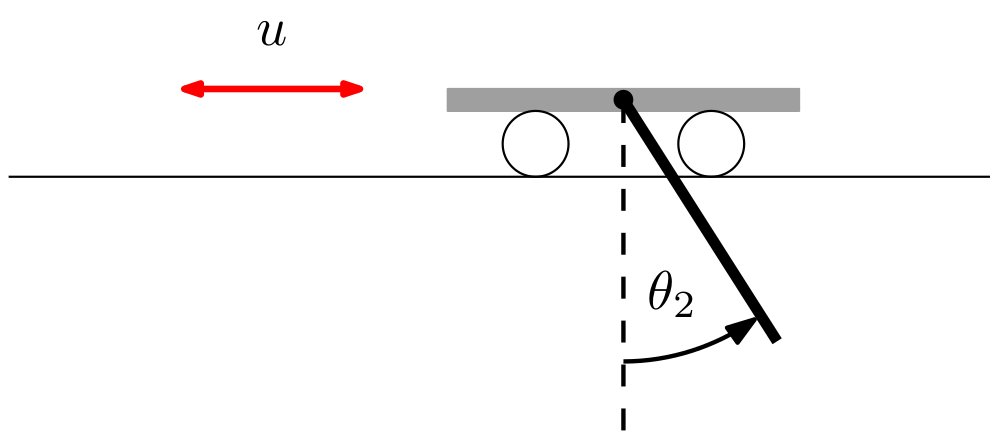
\includegraphics[width=0.5\textwidth]{Chapter3/Figures/cart-pole.png}
\caption[Cart-pole PILCO environment]{Cart-pole swing up. Source \cite{deisenroth2013pilco-documentation}.}
\label{Fig:cartpole-environment}
\end{figure}
The system has 4 continuous state variables: the position of the cart $x$, the velocity of the cart $\dot x$, the the pendulum angle $\theta_2$ and the angular velocity of the pendulum $\dot \theta_2$ of the pendulum. There is a target associated with each state variable.

\subsubsection{Pendubot}
The Pendubot shown in Fig. \ref{Fig:pendubot-environment}  is the second most complex environment used for experimentation. It consists of a central and outer pendulum of masses $m_1$ and $m_2$ and lengths $l_1$ and $l_2$, respectively. The two pendulums are linked together as well as the central pendulum being linked to the ground. The central and outer pendulum angles are given by $\theta_2$ and $\theta_3$, respectively, are measured anticlockwise from the upright vertical position. The link between the ground and the first pendulum can be actuated by the agent by applying a torque $u$ to the joint. The link between the pendulums cannot be actuated making the robot under actuated. The objective of the system is to actuate the central joint in such a way as to swing both pendulums to the upright vertical position and balanced there.
\begin{figure}[H]
\centering    
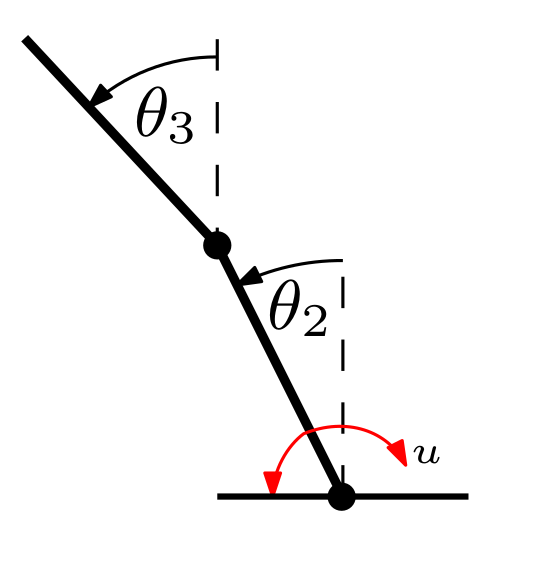
\includegraphics[width=0.25\textwidth]{Chapter3/Figures/pendubot.png}
\caption[Pendubot PILCO environment]{Source \cite{deisenroth2013pilco-documentation}.}
\label{Fig:pendubot-environment}
\end{figure}
The system has 4 continuous state variables: the angles of the pendulums $\theta_2$ and $theta_3$ and the angular velocities of the pendulums $\dot \theta_2$ and $\dot \theta_3$. There is a target associated with each state variable.

\subsubsection{Cart-Double-Pendulum}
The cart-double-pendulum shown in Fig. \ref{Fig:cartDoublePendulum-environment} is the most complex environment used for experimentation. It consists of a cart of mass $m_1$ and a central and outer pendulum of masses $m_2$ and $m_3$ and lengths $l_2$ and $l_3$, respectively. The two pendulums are linked together as well as the central pendulum being linked to the cart.  The central and outer pendulum angles are given by $\theta_2$ and $\theta_3$, respectively, and are measured anticlockwise from the upright vertical position. Continuous control actions $u$ applied to the cart cause it to move horizontally in the $x$-direction. The objective of the task is to actuate the cart in such a way that the double pendulum system is swung to the upright vertical position and balanced there while positioning the cart in the centre of the system at $x=0$. The unconstrained double pendulum system exhibits rich dynamical behaviour and is a chaotic system.
\begin{figure}[H]
\centering    
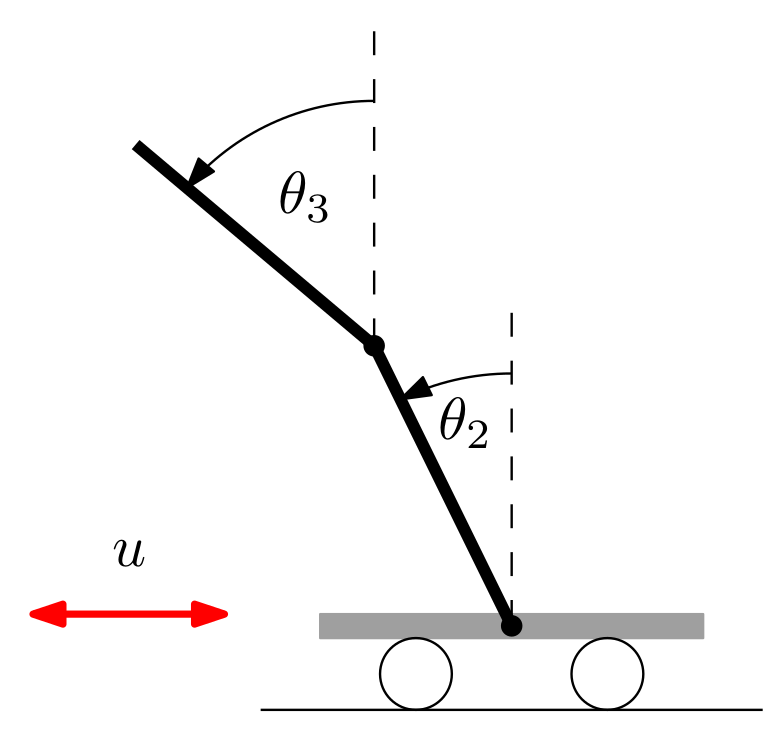
\includegraphics[width=0.3\textwidth]{Chapter3/Figures/cart-double-pendulum.png}
\caption[Cart-double-pendulum PILCO environment]{Source \cite{deisenroth2013pilco-documentation}.}
\label{Fig:cartDoublePendulum-environment}
\end{figure}
The system has 6 continuous state variables: the position of the cart $x$, the velocity of the cart $\dot x$, the angles of the pendulums $\theta_2$ and $theta_3$ the angular velocities of the pendulums $\dot \theta_2$ and $\dot \theta_3$. There is a target associated with each state variable.


\section{Experimental Results}

\subsection{The Evolution of Distributions over States and Costs}
The Monte-Carlo uncertainty estimates are performed by rolling out state-action values through the dynamics model using the one-step predictions in Eq. \ref{Eq:model-posterior-one-step} and for each state visited a cost is calculated with Eq. \ref{Eq:PILCO-cost-function} . PILCO's direct policy search method is formulated so that the cost is directly consulted when deciding a policy (see Eq \ref{Eq:PILCO-expected-return}) and not the state itself (although the cost is a function of the state). It is therefore important illustrate the difference by observing how the distribution over states and the distribution over costs evolve as they are propagated through the model in the context of the Monte-Carlo method presented in Section \ref{S:monte-carlo-estimate}.

This is demonstrated by performing $9$ steps through the simple $1$\textit{-dimensional} transition function shown in Fig. \ref{Fig:1-dimensional-transition-function}. The transition function represents the input space $\mathbf{x}_{t}\in [-5, 5]$ and is trained on targets representing the next state $\mathbf{x}_{t+1}$, not state differences as is done with PILCO. Fig. \ref{Fig:1-dimensional-transition-function} shows the trigonometric basis function model's predictive mean and $95\%$ confidence interval over observed state transitions and $4$ functions drawn from the posterior distribution over the model weights $q(\mathbf{w})$. To illustrate the evolution of state and cost distributions for the first step through the transition function, $M=1000$ sets of weights $\mathbf{w} \sim q(\mathbf{w})$ were sampled and for each set, $N=1000$ starting states drawn from $\mathbf{x}_{0} \sim \mathcal{U}(-5,5)$ were stepped through the function according to Eq. \ref{Eq:model-posterior-one-step}. This process was repeated $8$ more times but for each step, the next state $\mathbf{x}_{t+1}$ as predicted by Eq. \ref{Eq:model-posterior-one-step} was fed back into the equation as the input state $\mathbf{x}_{t}$. At each step the cost was calculated with Eq. \ref{Eq:PILCO-cost-function} with width $\sigma_{c}=1.5$ and target state $\mathbf{x}_{\text{target}}=0$. There is no explicit policy used here. This can be viewed as if there is only one action and the agent selects that action at each opportunity. This enables the states and costs to evolve freely under the system dynamics.

\begin{figure}[htp!]
\centering    
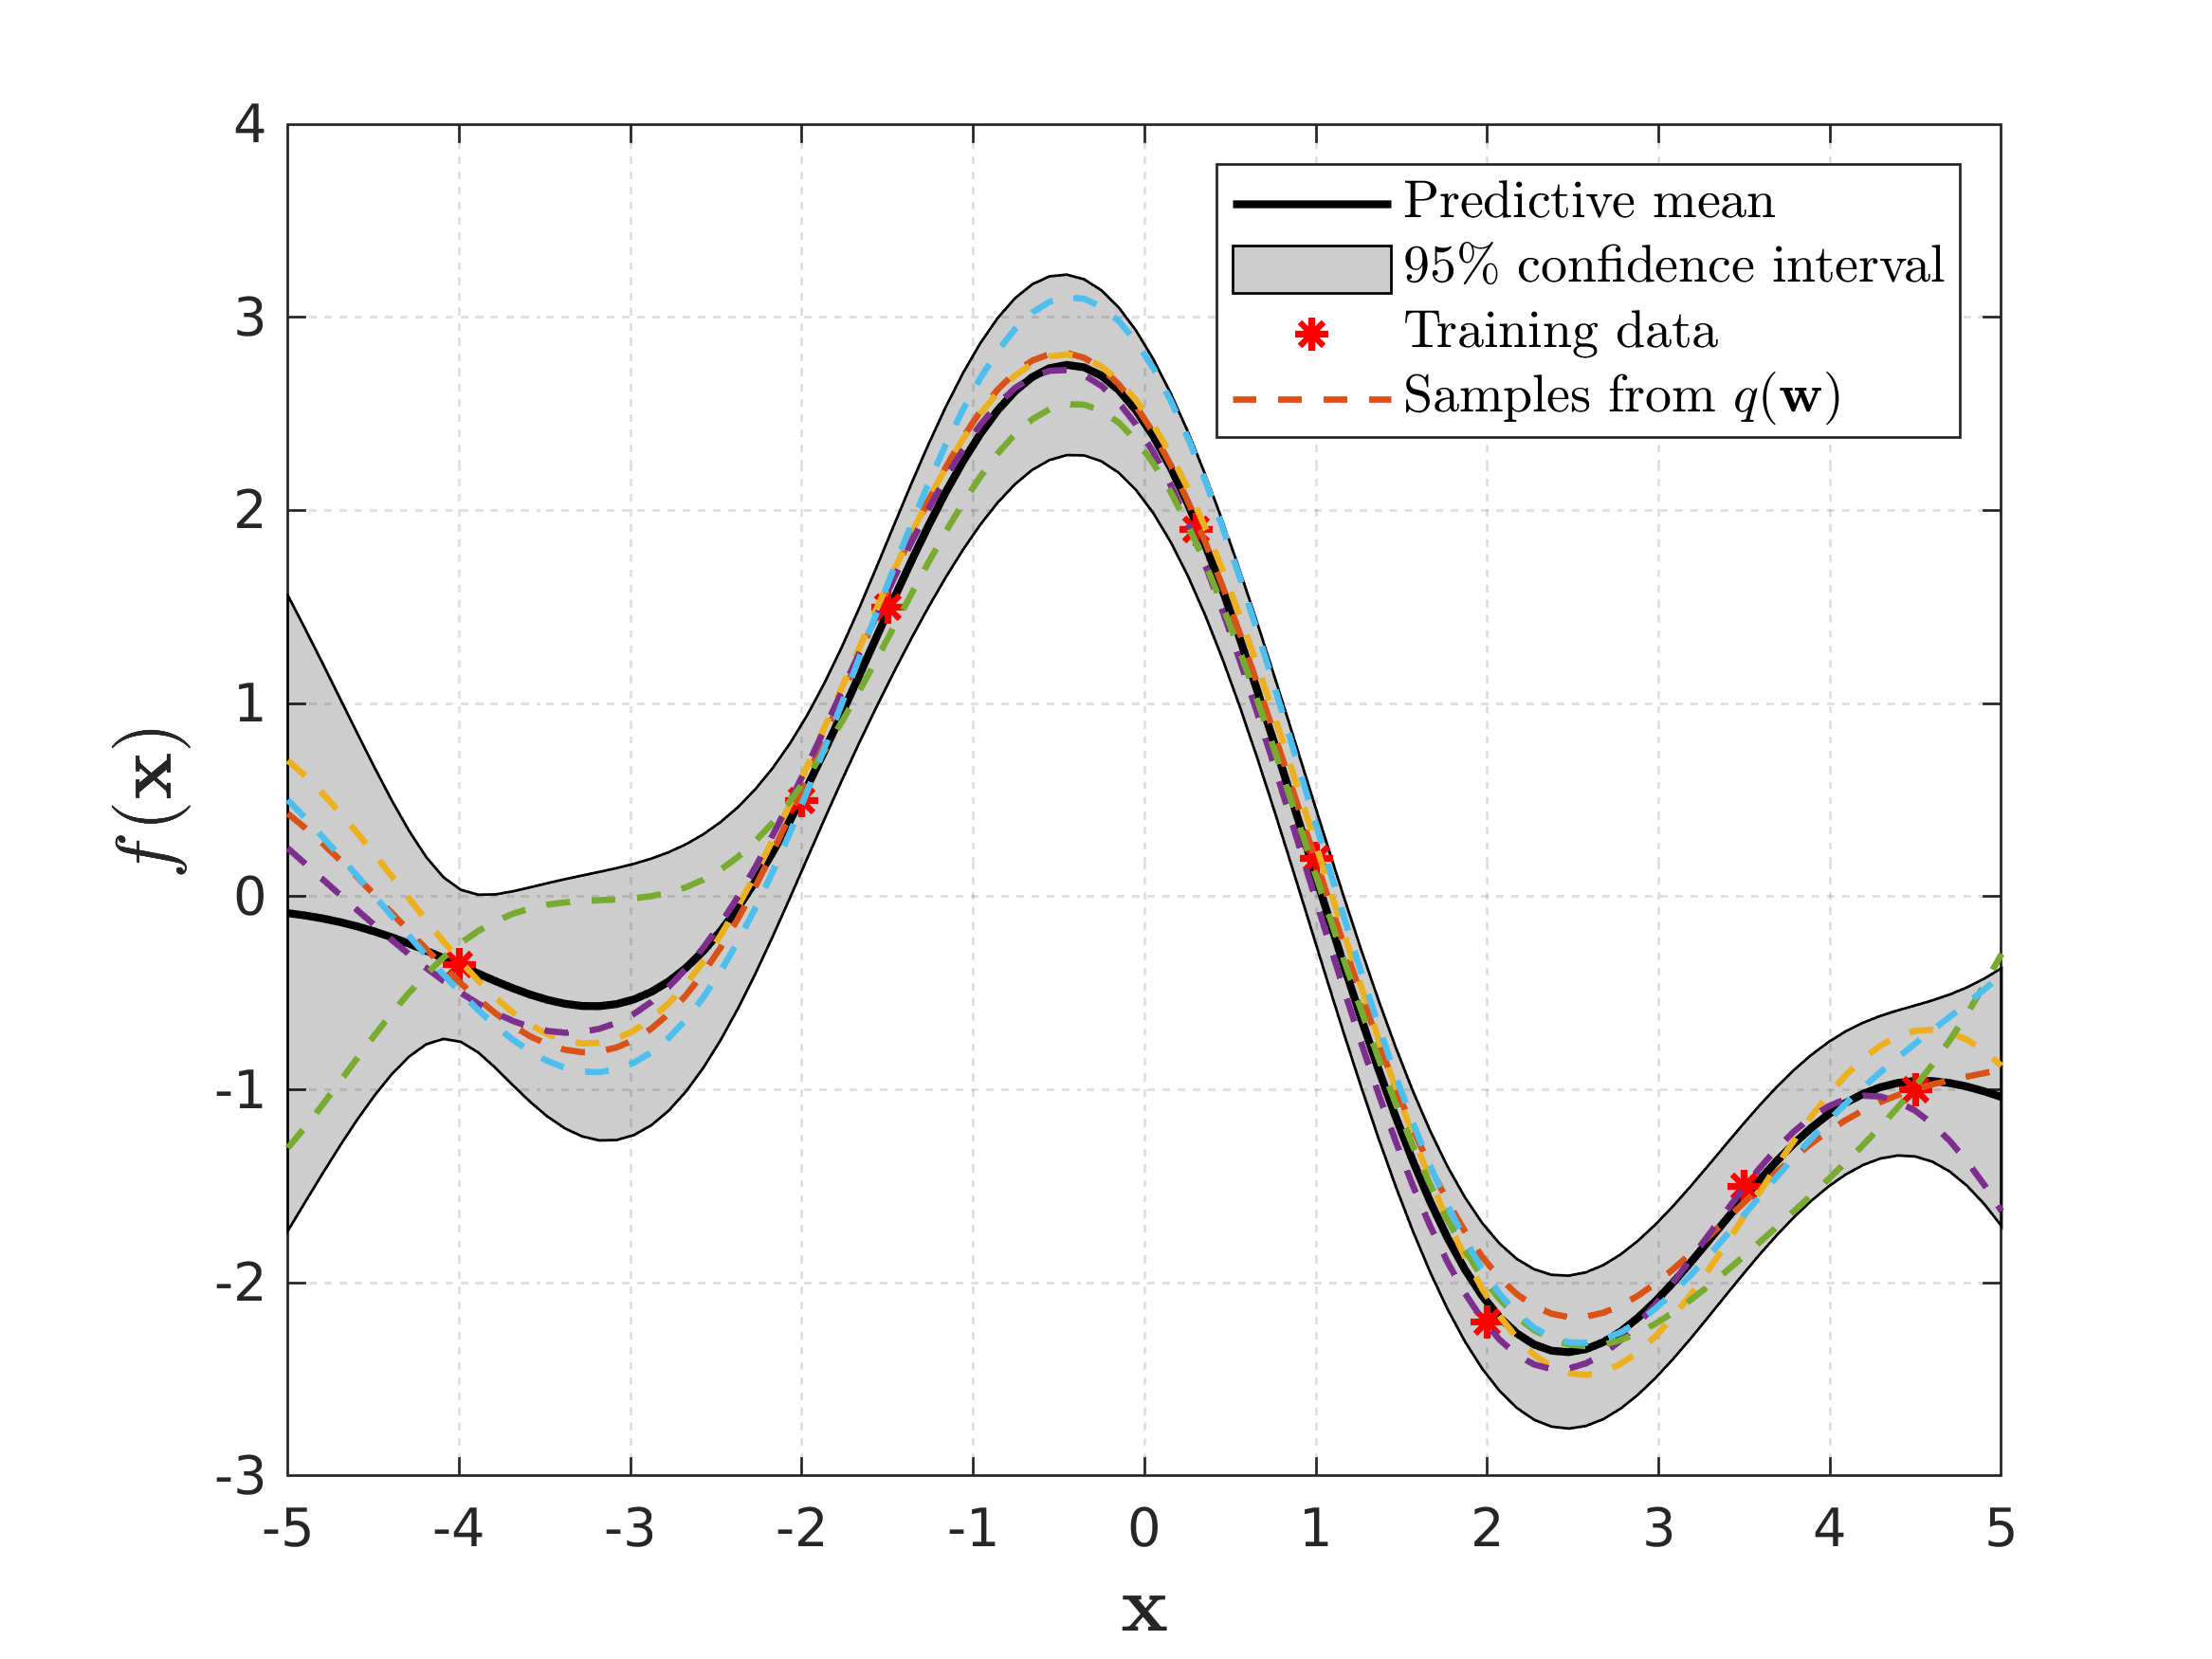
\includegraphics[width=0.6\textwidth]{Chapter3/Figures/transition_function.png}
\caption[A 1-dimensional transition function example]{A 1-dimensional transition function example}
\label{Fig:1-dimensional-transition-function}
\end{figure}

Fig \ref{Fig:Re-evolution-of-state-and-cost} shows the evolution of the distributions over states and costs for input distributions (\ref{Fig:Re-hist-traj-1} and \ref{Fig:Re-hist-cost-1}), after 1 transition (\ref{Fig:Re-hist-traj-2} and \ref{Fig:Re-hist-cost-2}) and 9 transitions (\ref{Fig:Re-hist-traj-4} and \ref{Fig:Re-hist-cost-4}). The distribution over costs associated with the initial distribution over states reveals the locally quadratic nature of the cost function where the high density at $\mathbb{C}(x)=1$ indicates saturation of costs associated with states further away from the target state. After the first step, the distribution over states tightens around the target state with a peak about $\mathbf{x}=-0.7$. The reduction in the state distribution tails means that the cost no longer saturates and the tightening around the target state has increased the cost density about $\mathbb{C}(\mathbf{x})=0$. Finally, after 9 steps, the state distribution flattens out with small peaks around the $\pm\mathbf{x}=2$. The high density about $\mathbb{C}(x)=0$ reduces and a bump forms about the $\mathbb{C}(x)=0.8$ position corresponding the peaks of the state distribution. 
\begin{figure}[htp!]    
  \begin{subfigure}[b]{0.49\linewidth}
    \centering
    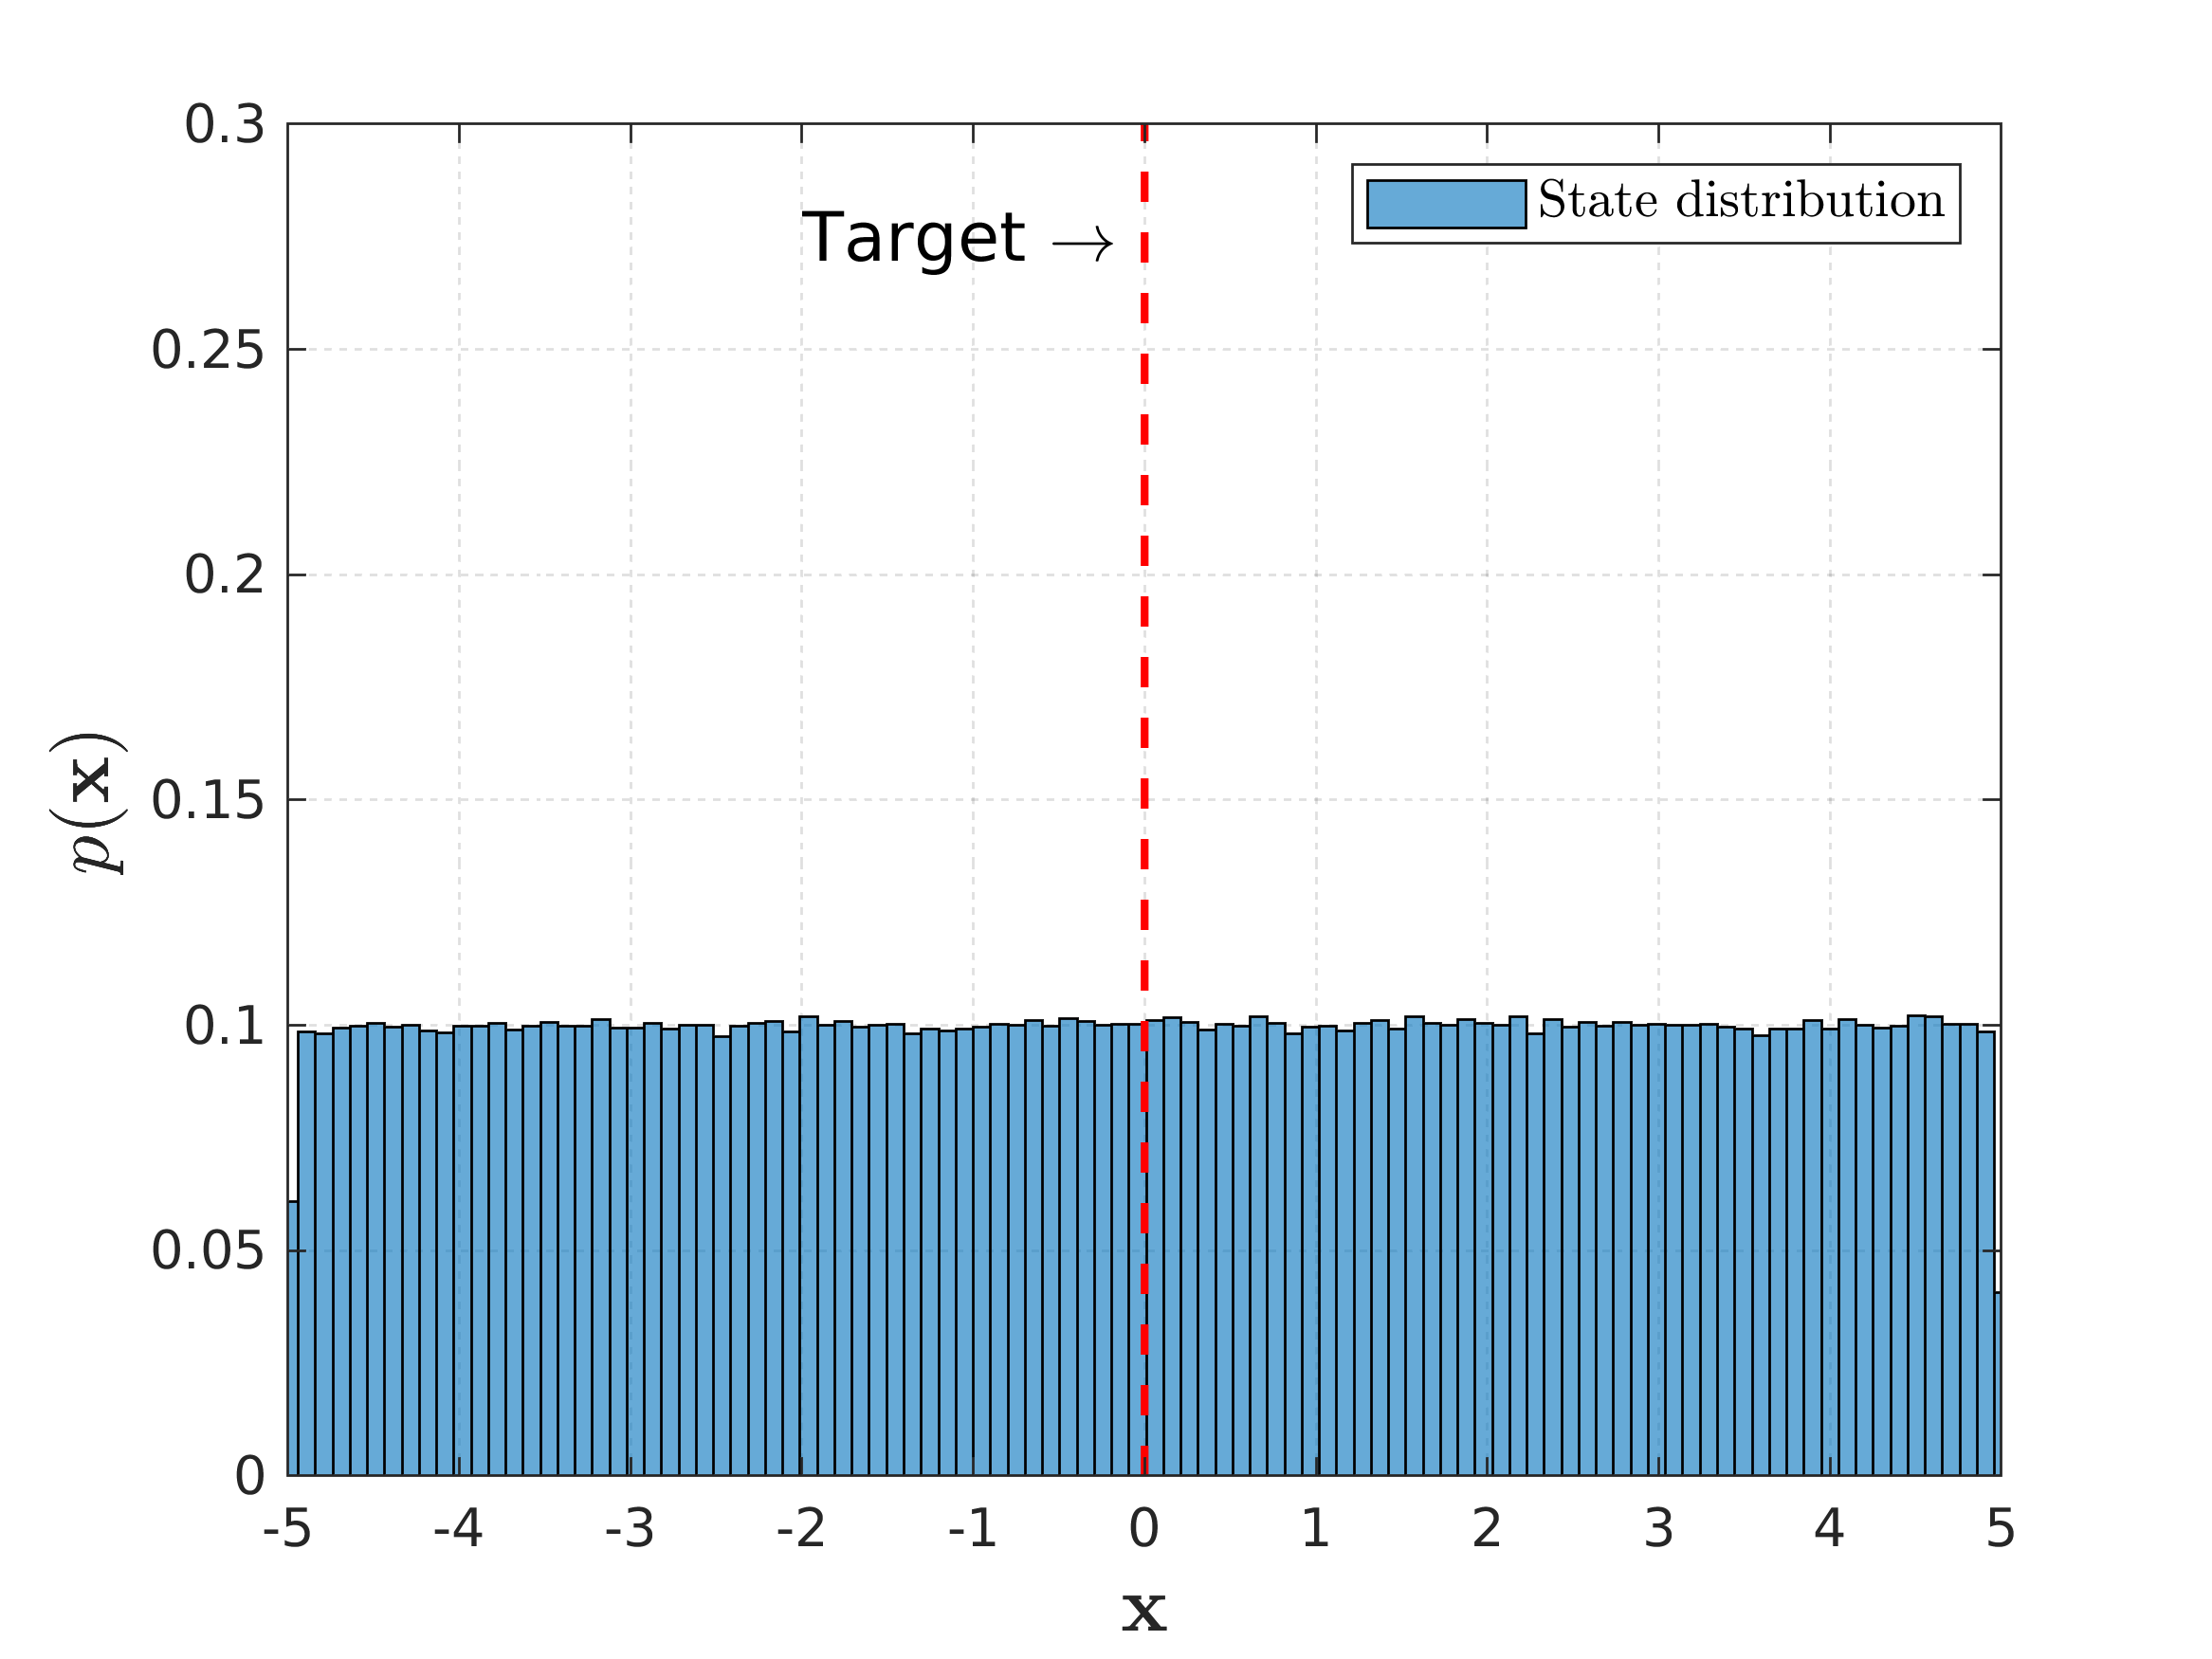
\includegraphics[height=0.25\textheight,width=1\textwidth]{Chapter3/Figures/trans_traj_hist_1.png} 
    \caption{Input distribution over states} 
    \label{Fig:Re-hist-traj-1} 
  \end{subfigure} 
%   \hspace{\fill}  %% maximize space between adjacent subfigures
  \begin{subfigure}[b]{0.49\linewidth}
    \centering
    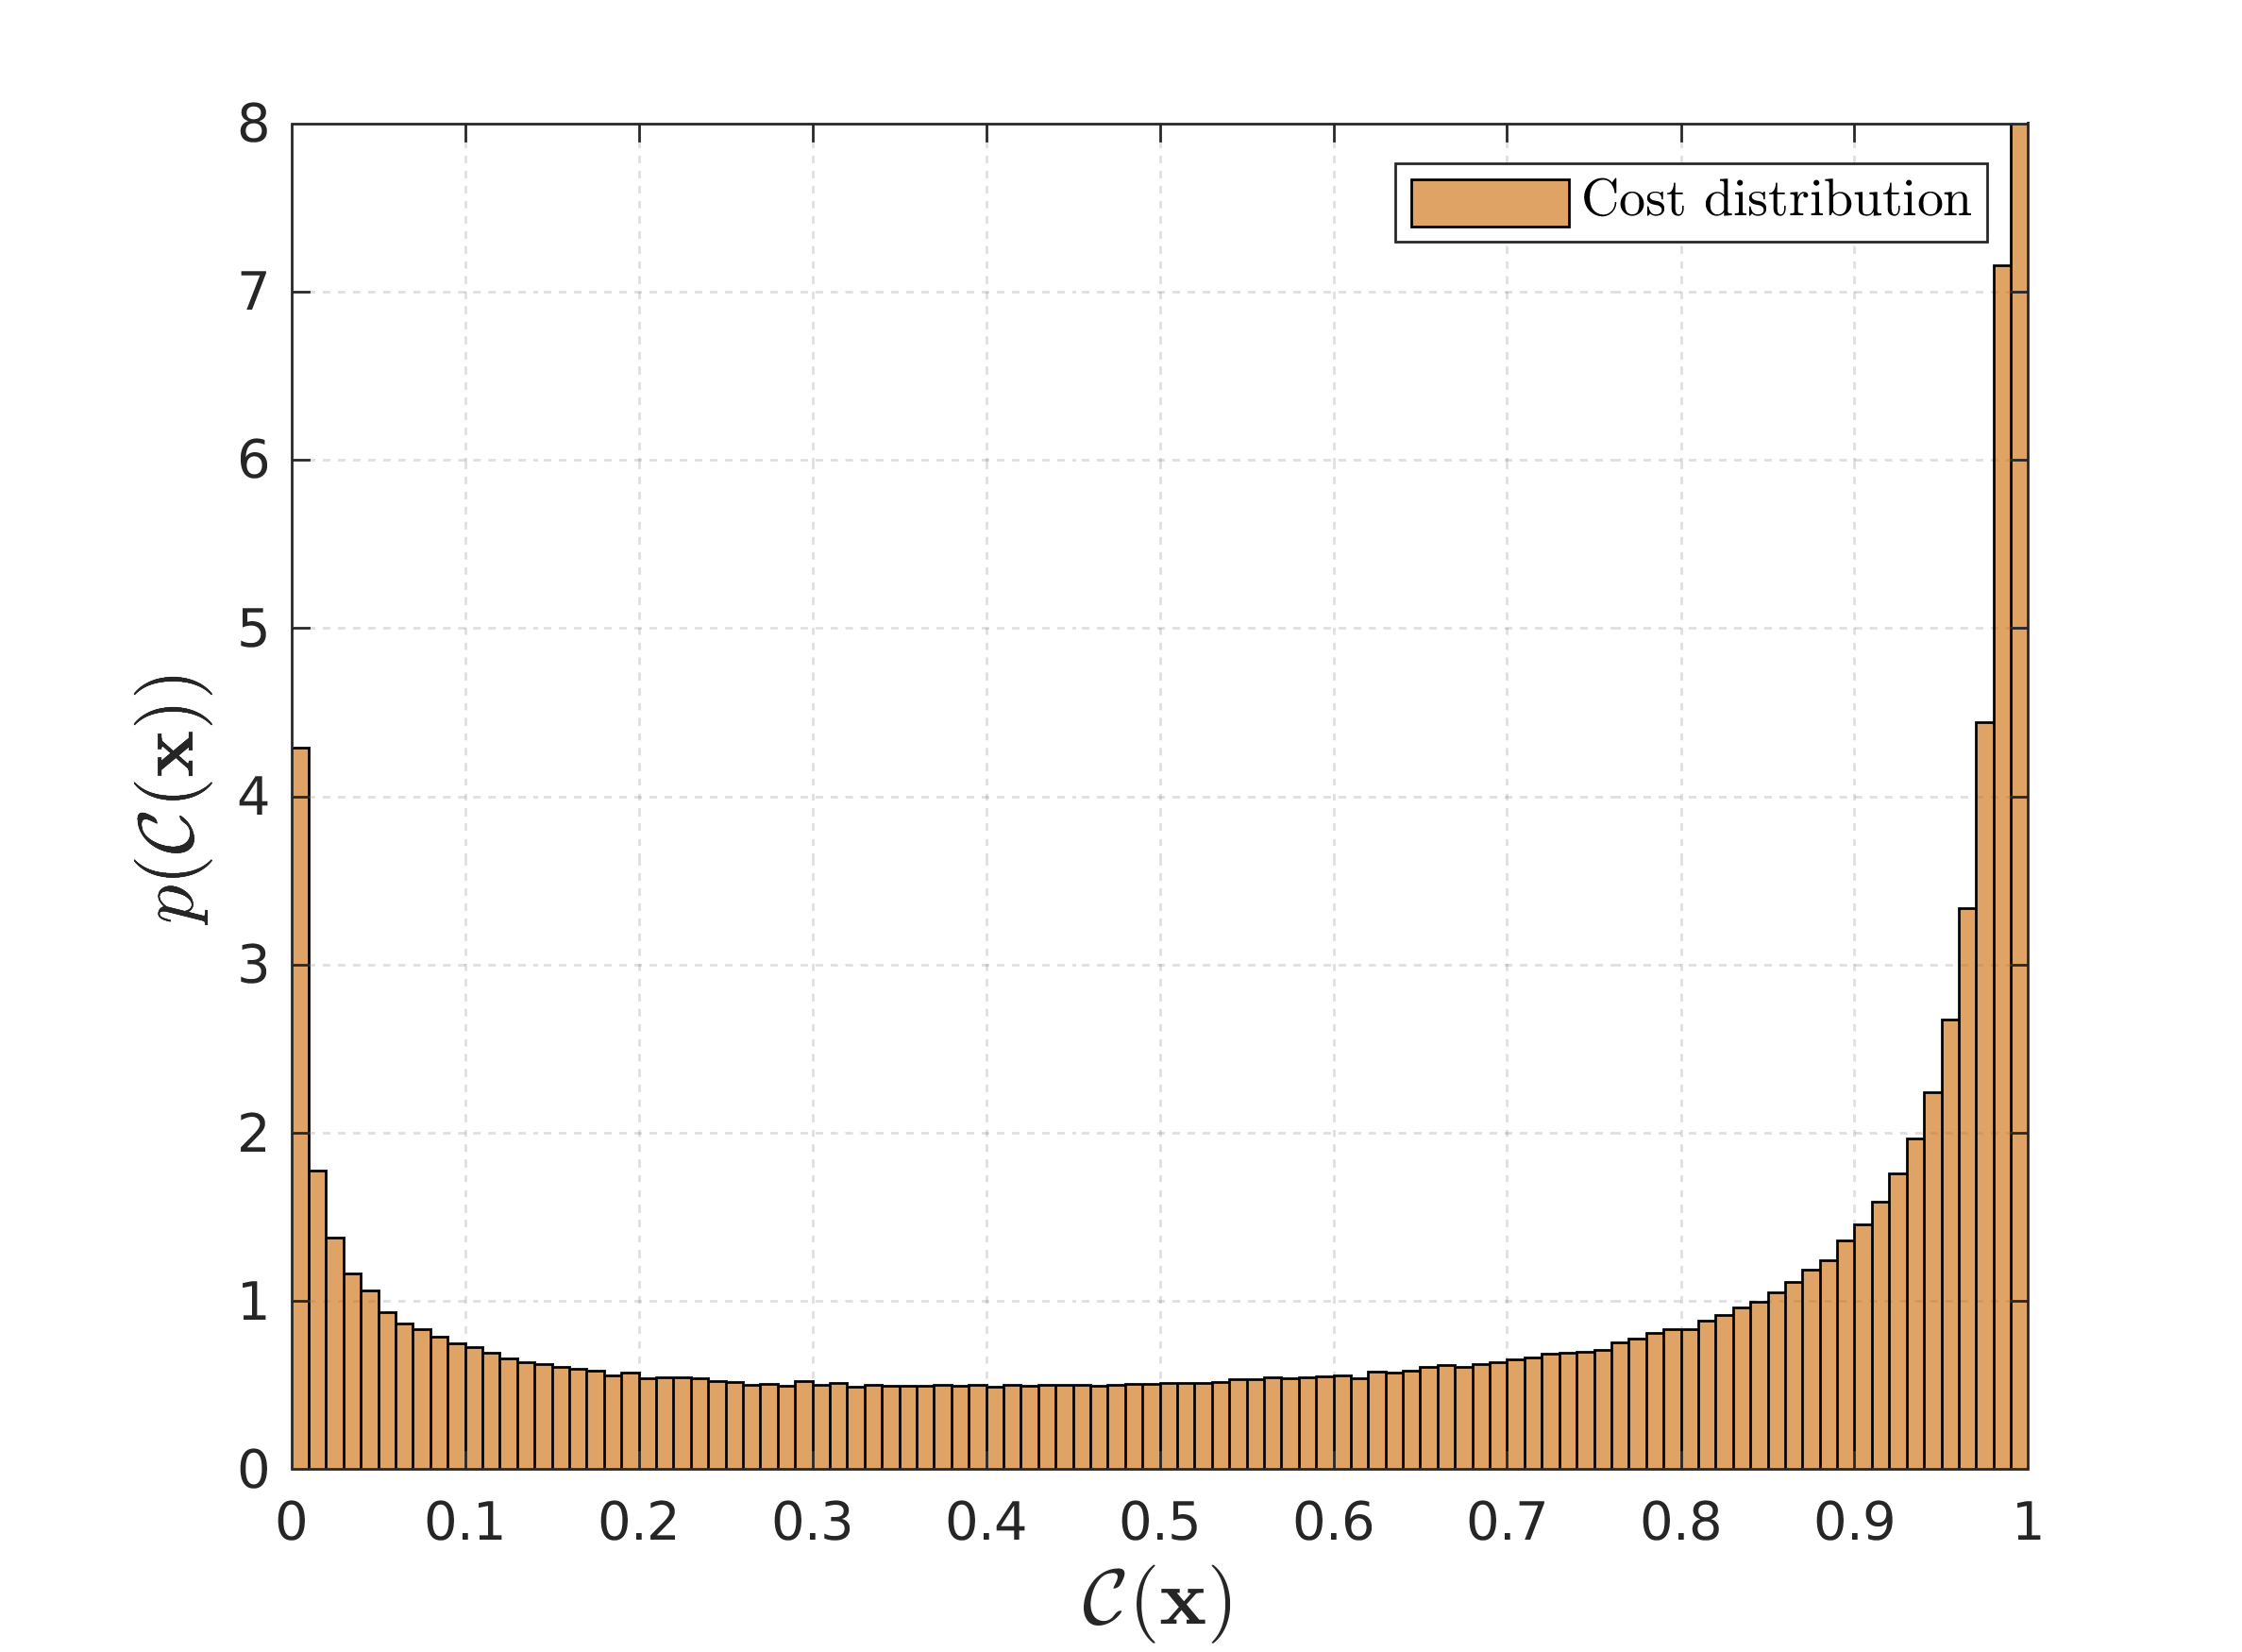
\includegraphics[height=0.25\textheight,width=1\textwidth]{Chapter3/Figures/trans_cost_hist_1.png} 
    \caption{Input distribution over costs} 
    \label{Fig:Re-hist-cost-1} 
  \end{subfigure} 

%   \vspace{4ex}  %% extra vertical space
  \begin{subfigure}[b]{0.49\linewidth}
    \centering
    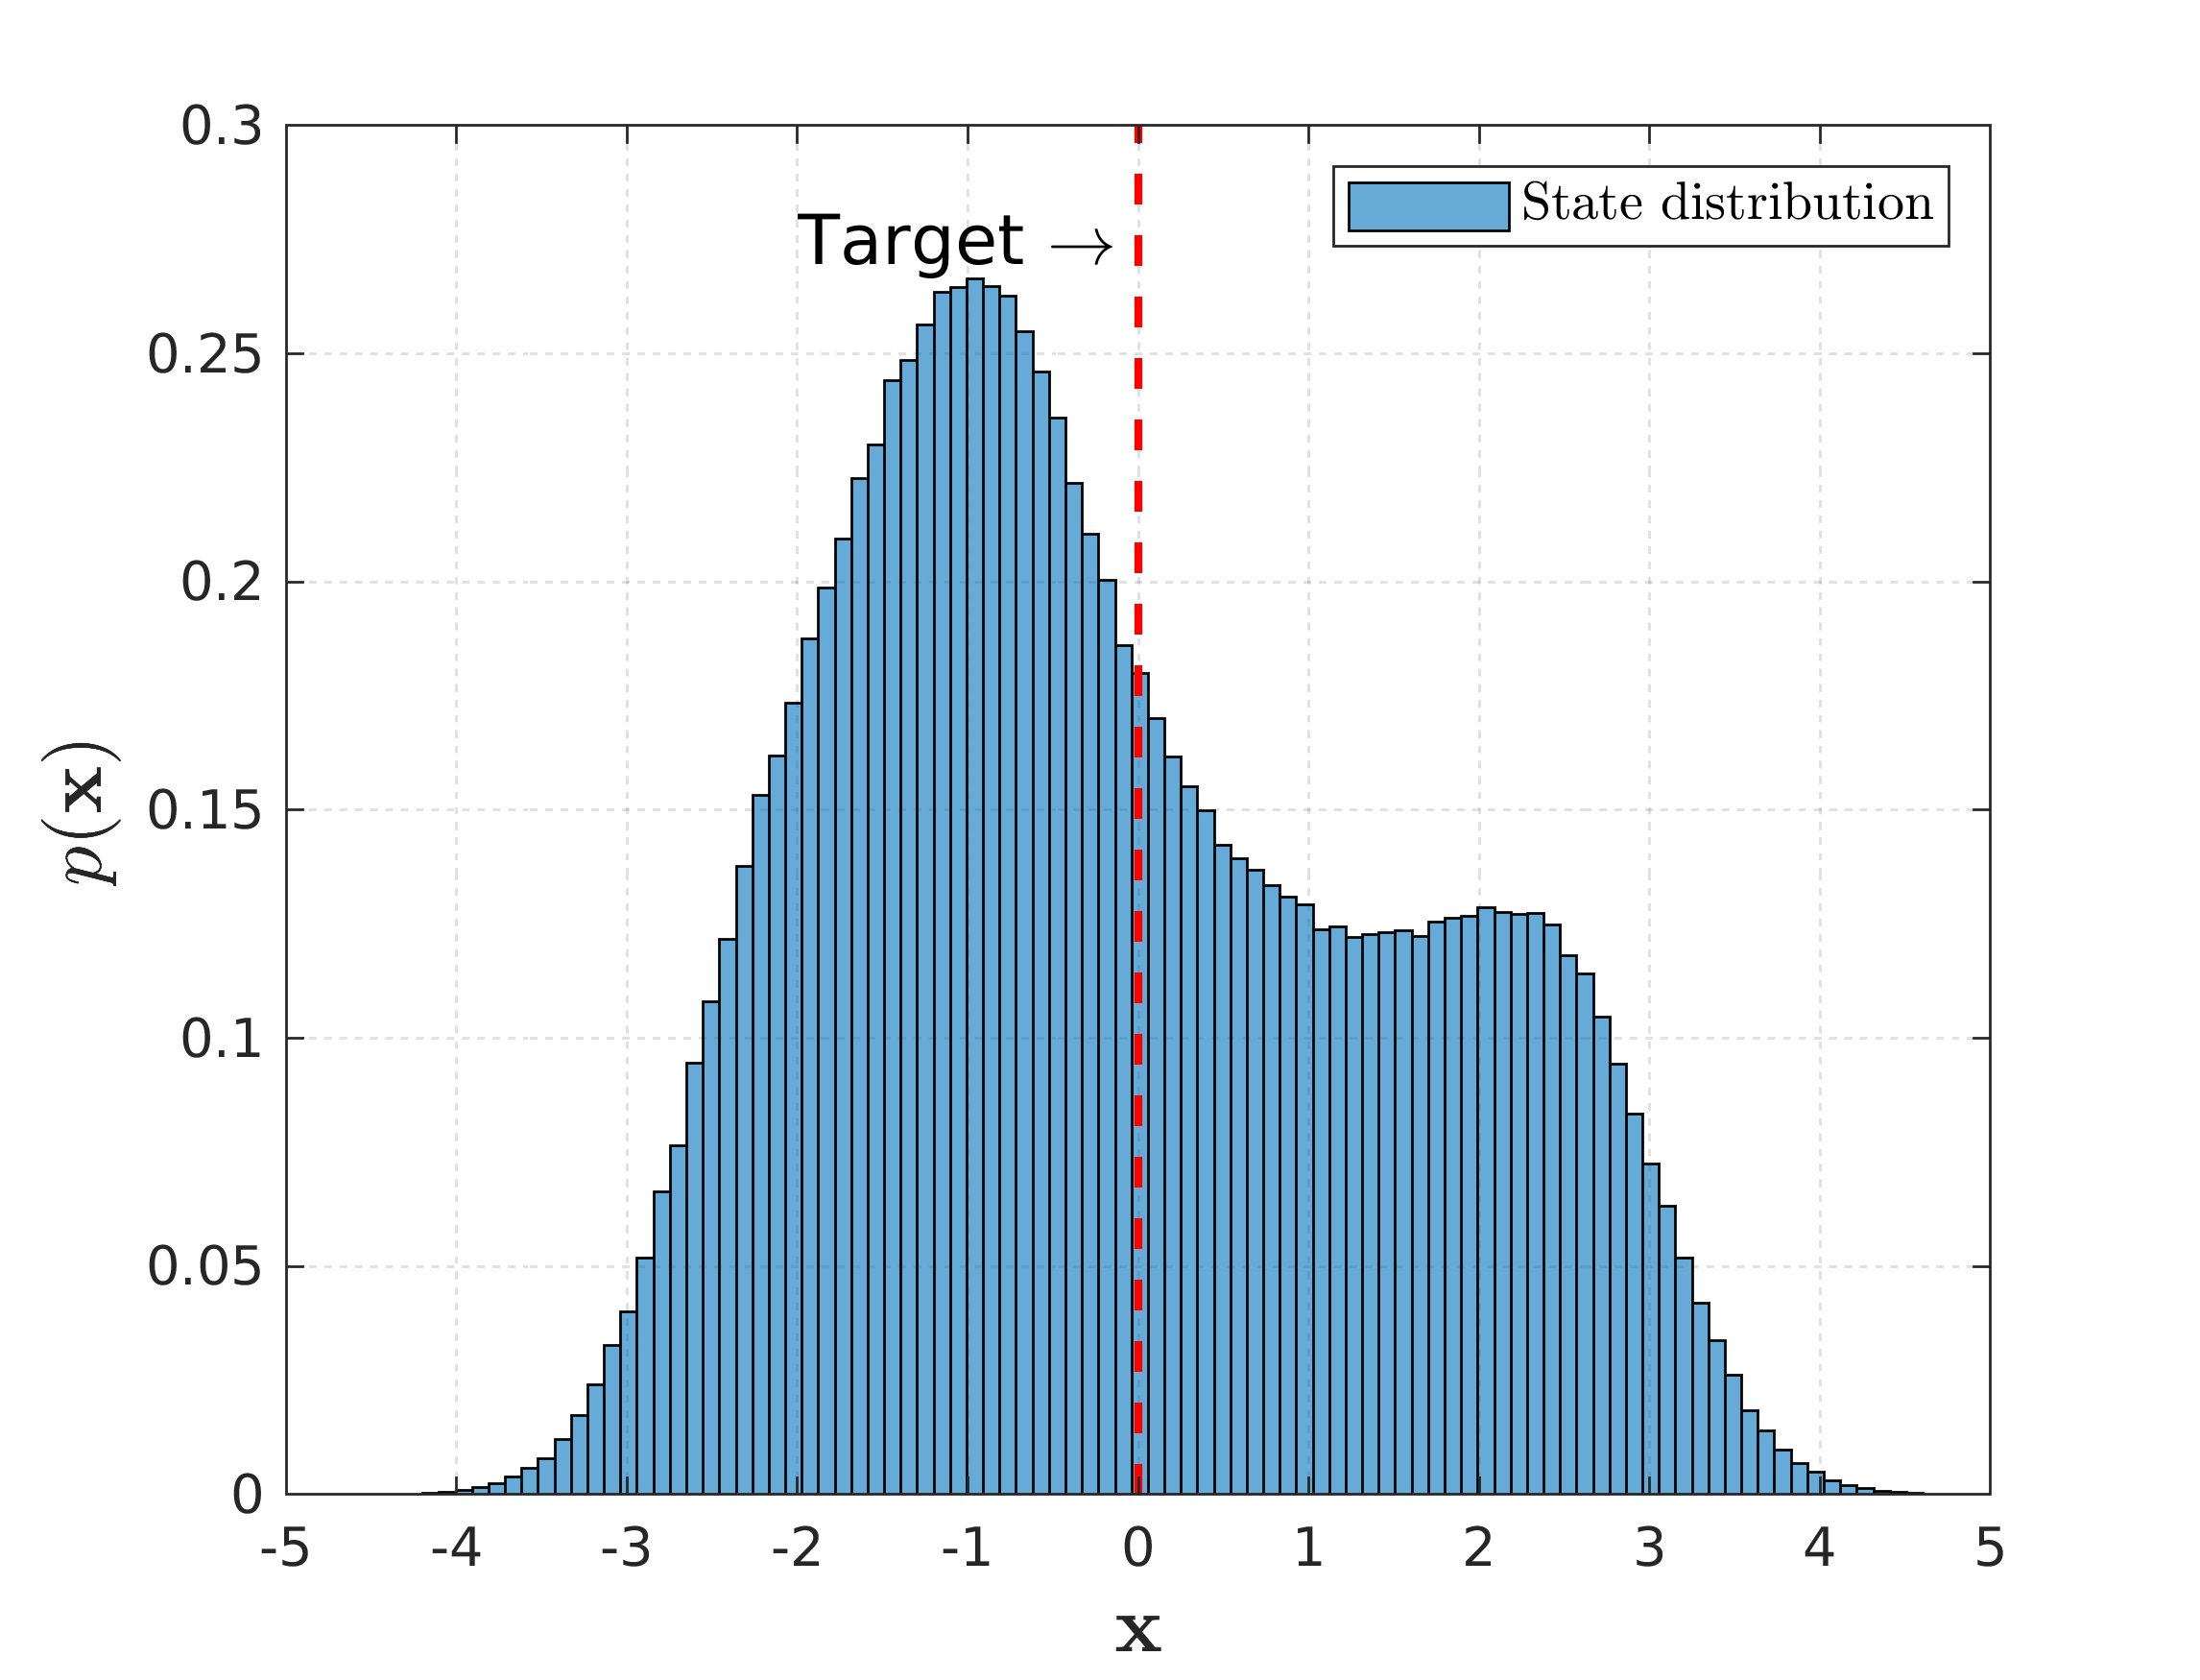
\includegraphics[height=0.25\textheight,width=1\textwidth]{Chapter3/Figures/trans_traj_hist_2.png} 
    \caption{Distribution over states after 1 transition} 
    \label{Fig:Re-hist-traj-2} 
  \end{subfigure} 
%   \hspace{\fill}
  \begin{subfigure}[b]{0.49\linewidth}
    \centering
    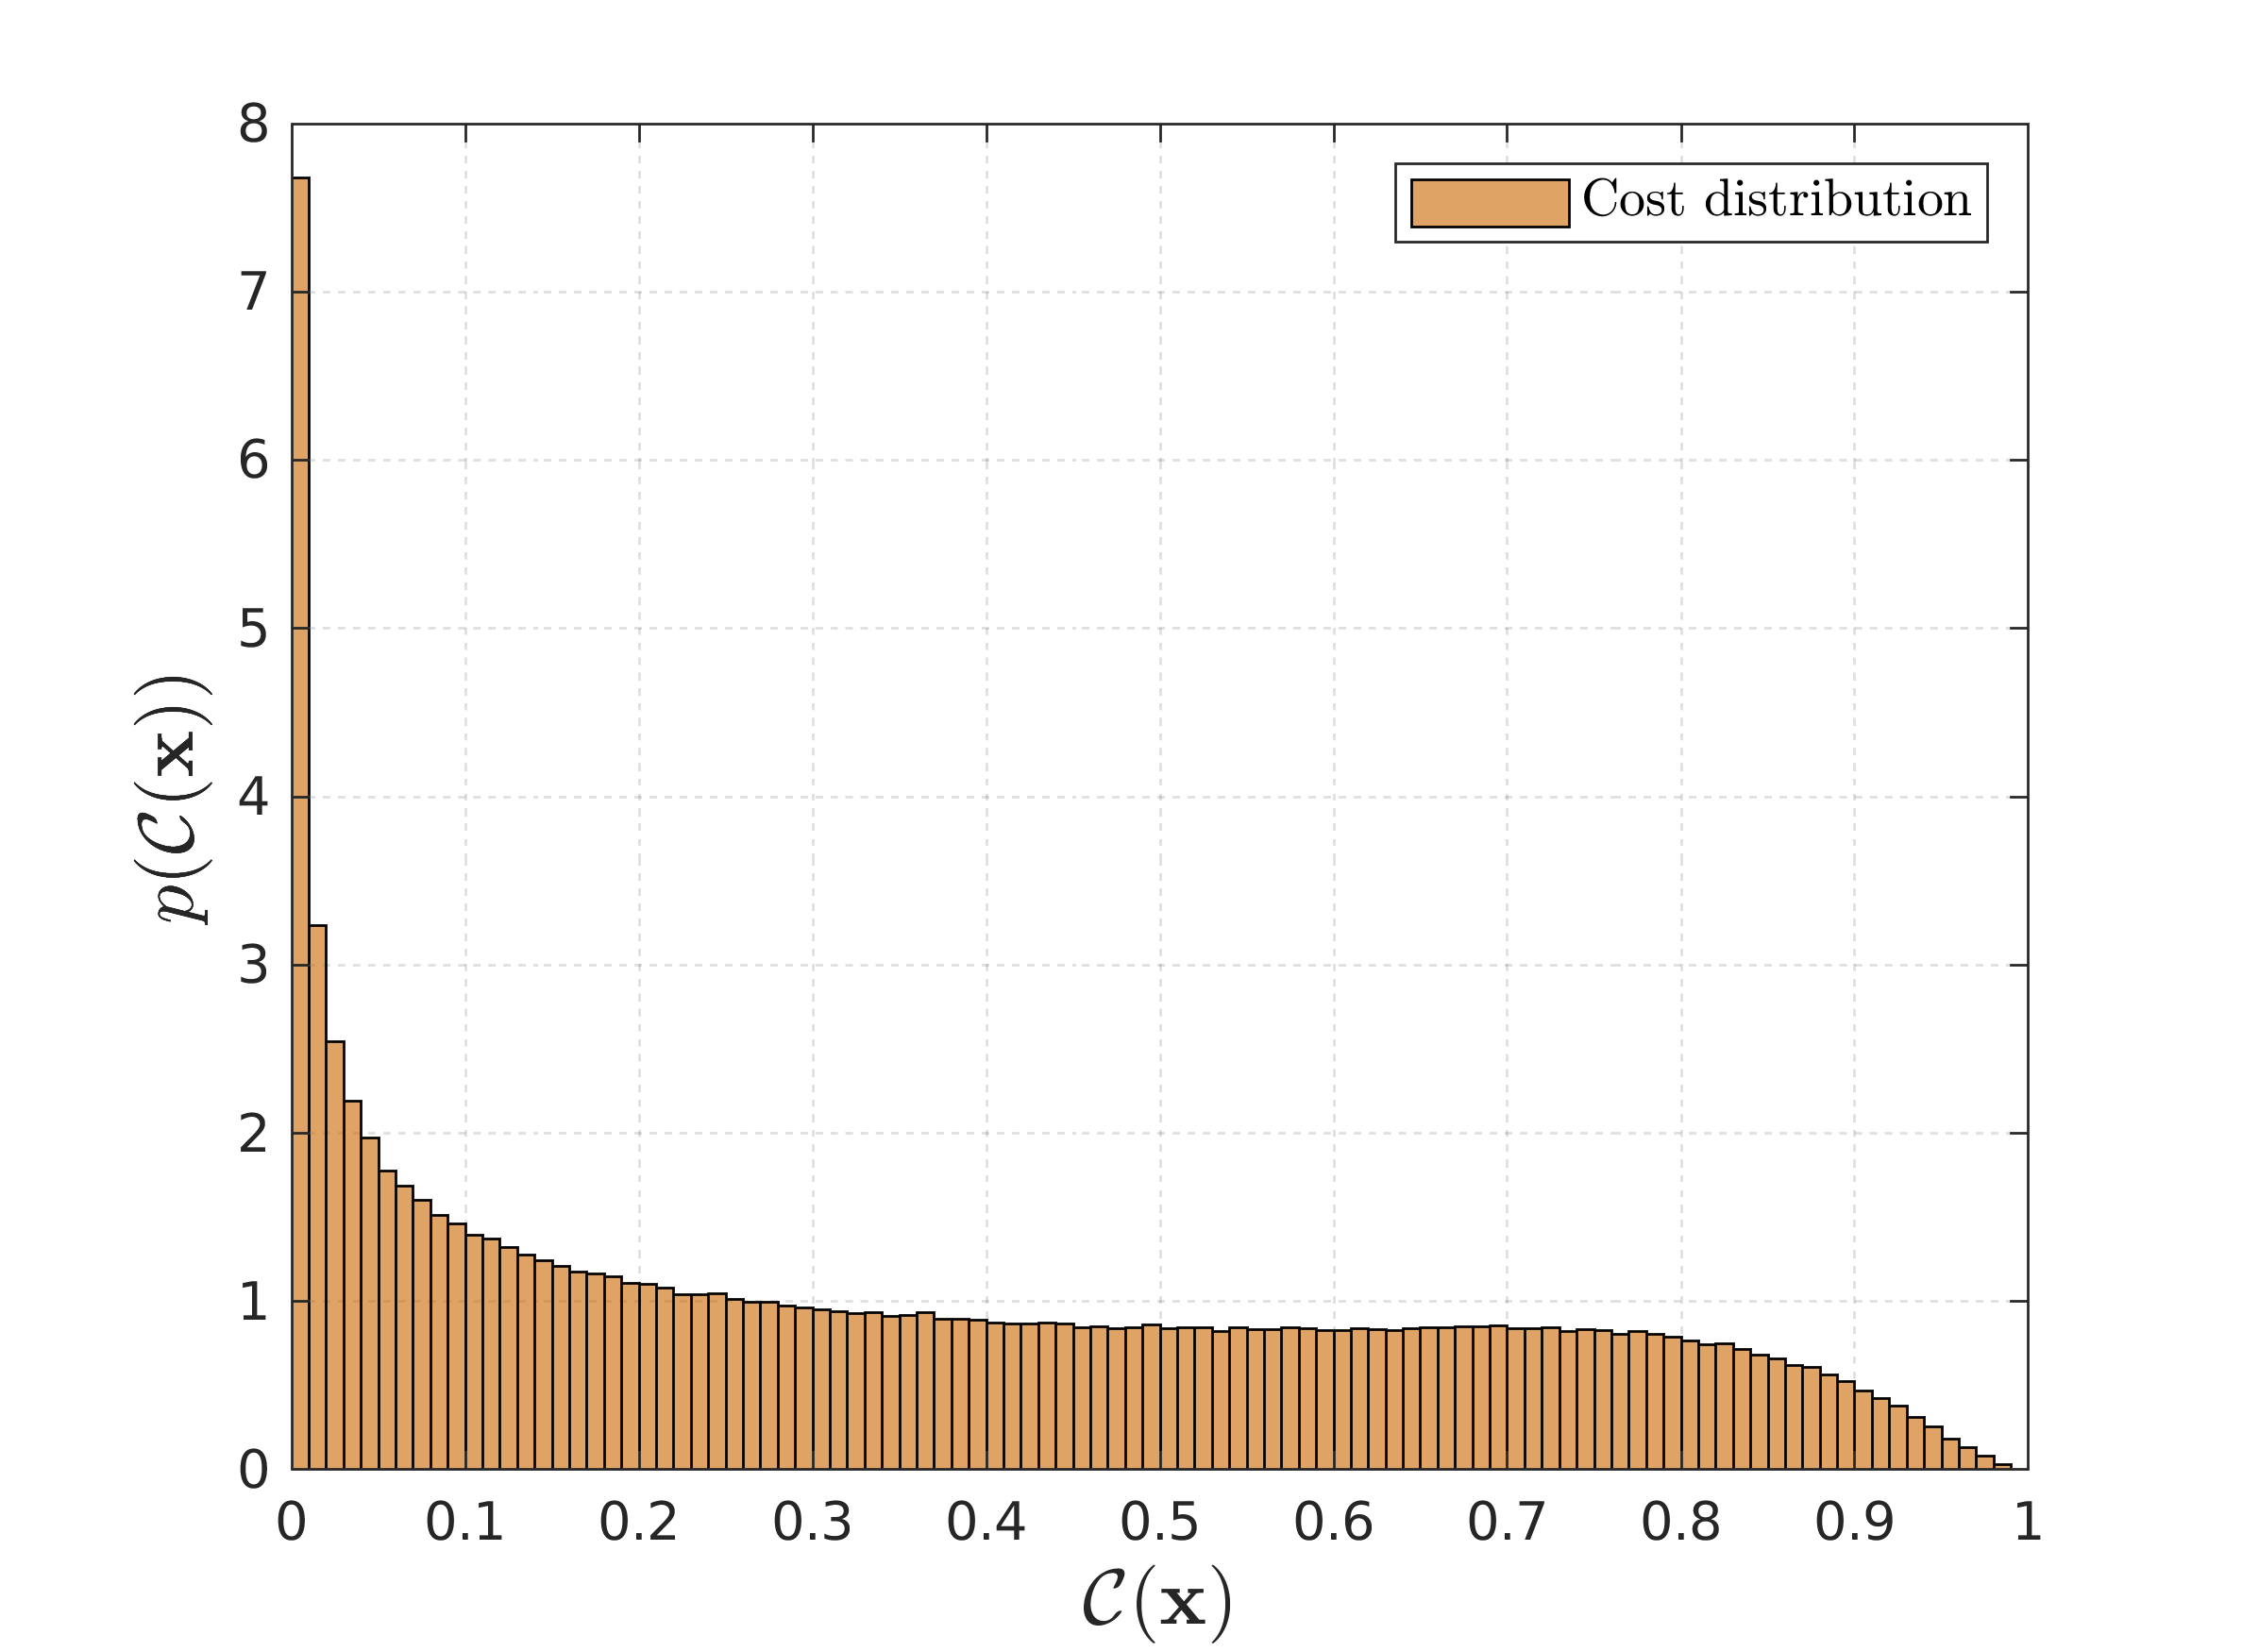
\includegraphics[height=0.25\textheight,width=1\textwidth]{Chapter3/Figures/trans_cost_hist_2.png} 
    \caption{Distribution over costs after 1 transition} 
    \label{Fig:Re-hist-cost-2} 
  \end{subfigure} 

    % \vspace{4ex}
  \begin{subfigure}[b]{0.49\linewidth}
    \centering
    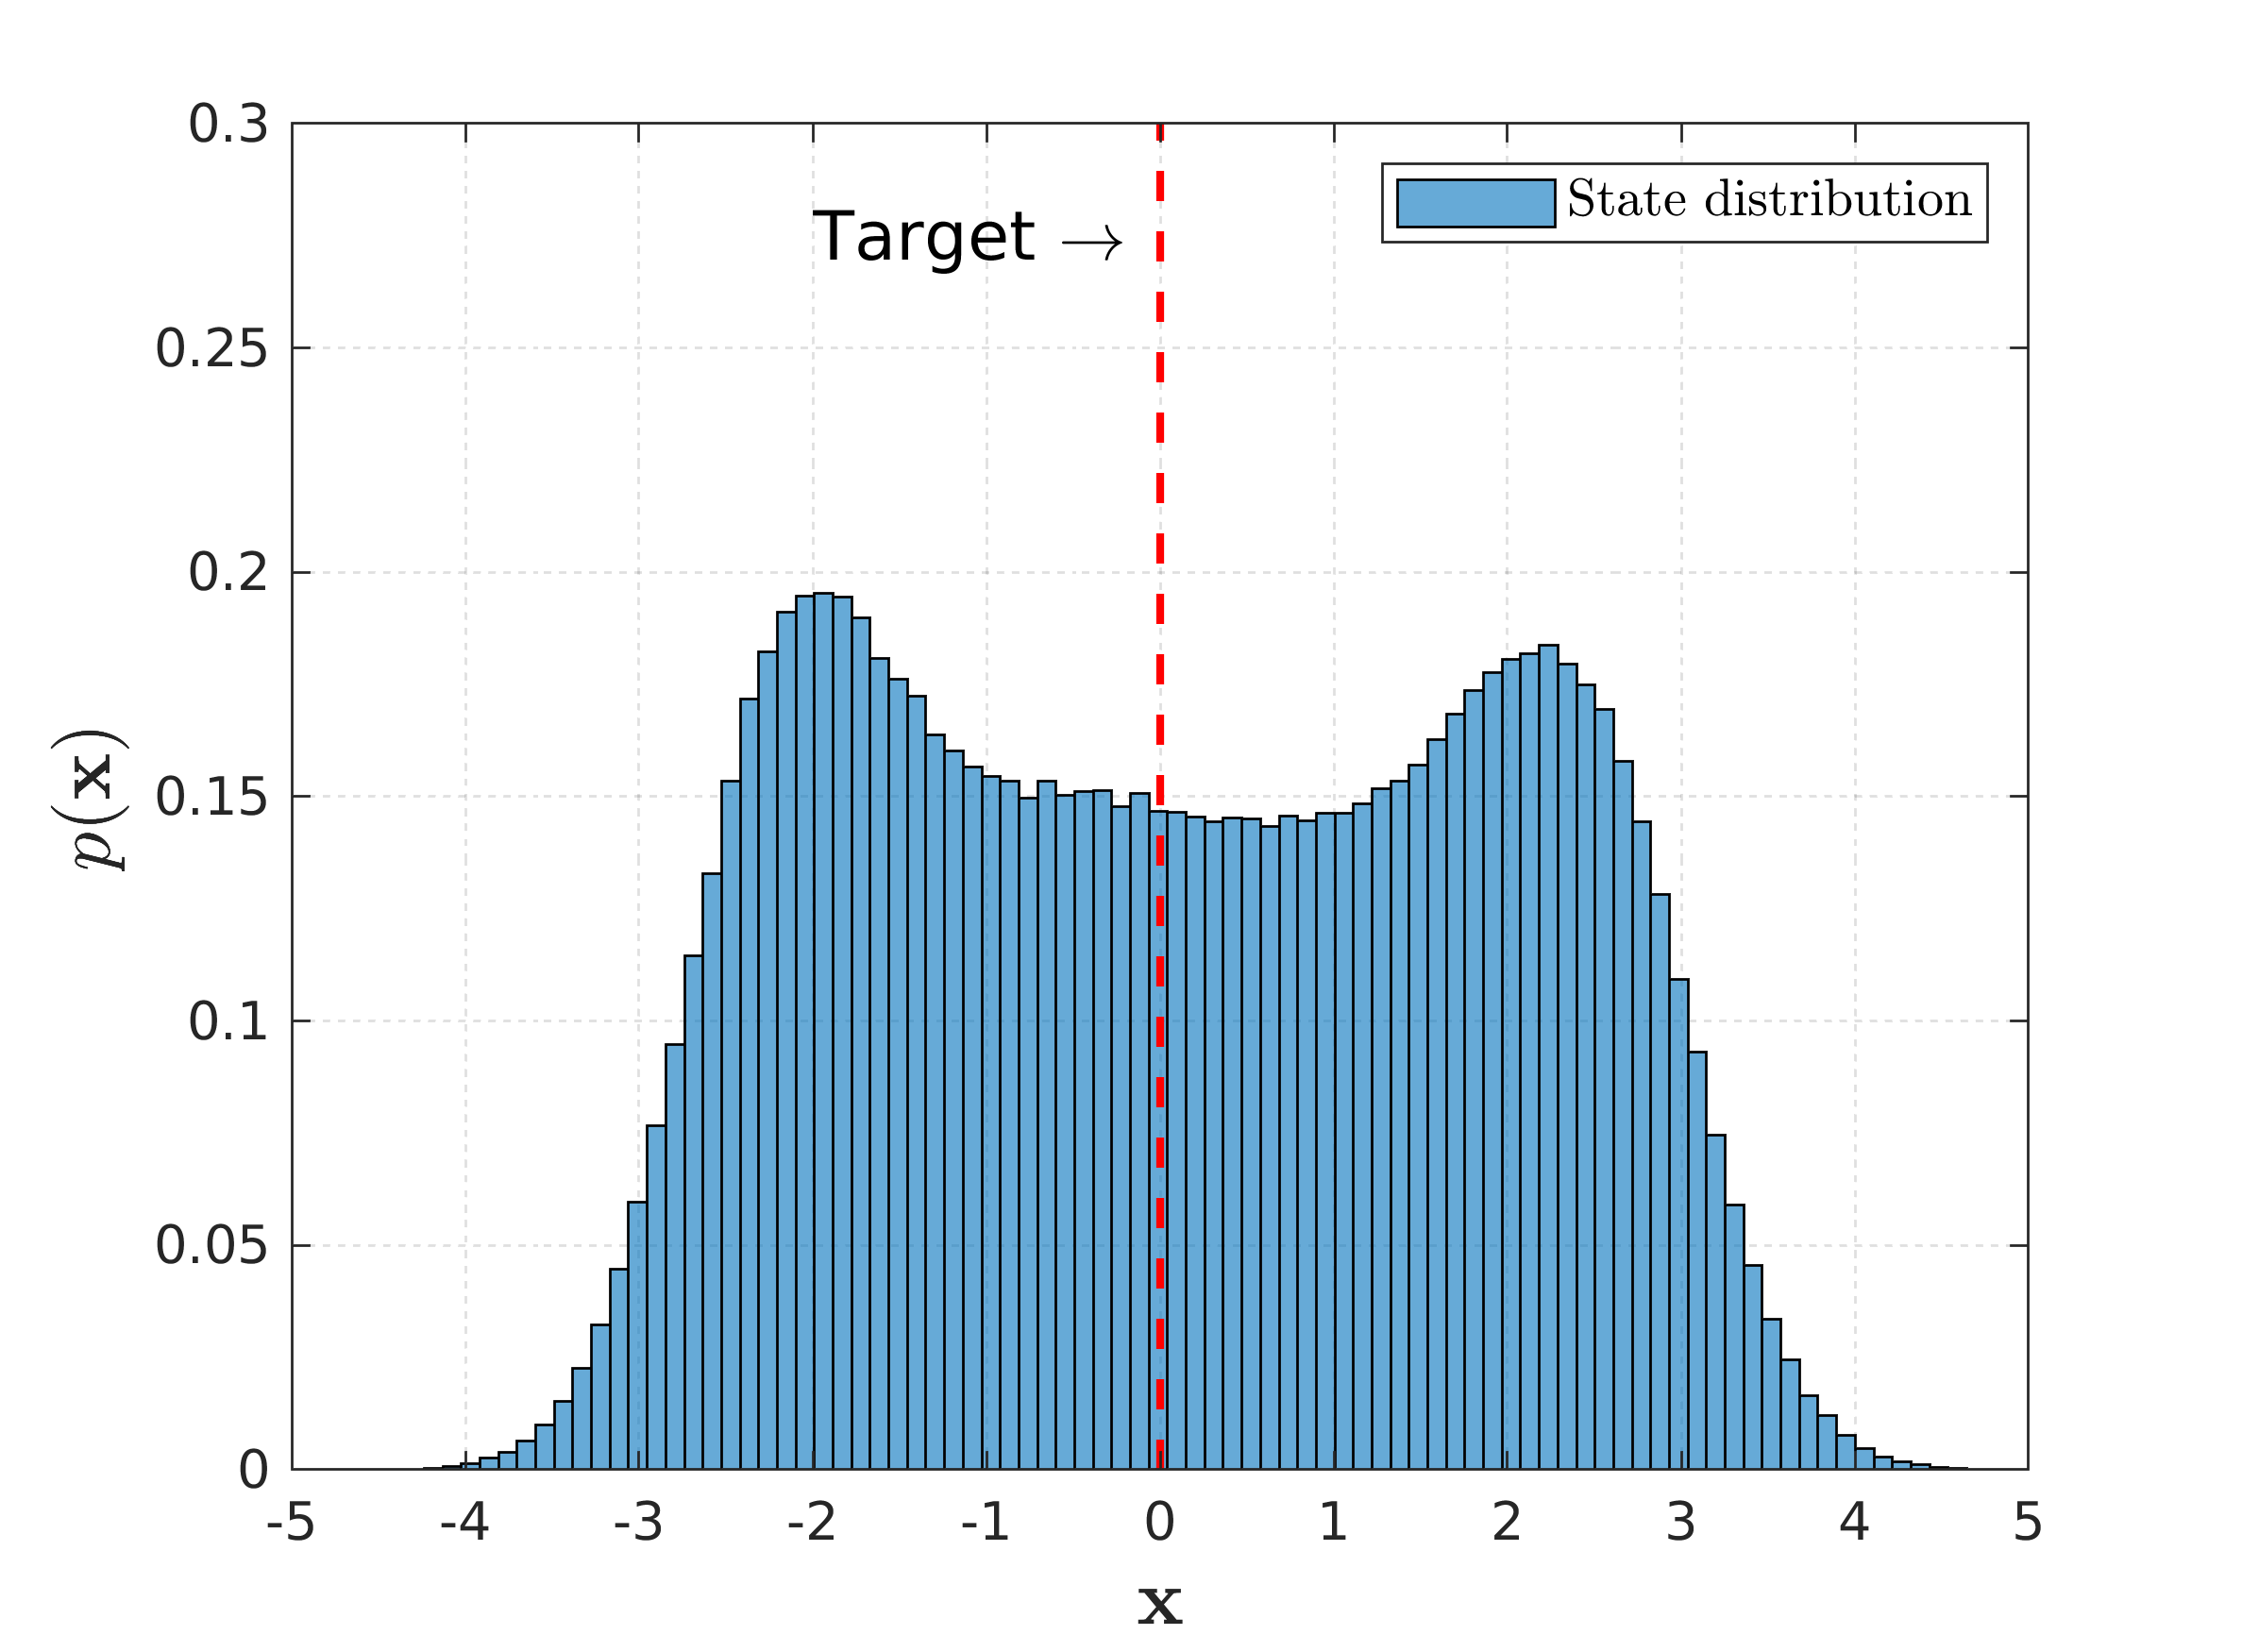
\includegraphics[height=0.25\textheight,width=1\textwidth]{Chapter3/Figures/trans_traj_hist_4.png} 
    \caption{Distribution over states after 9 transitions} 
    \label{Fig:Re-hist-traj-4} 
  \end{subfigure}
%   \hspace{\fill}
  \begin{subfigure}[b]{0.49\linewidth}
    \centering
    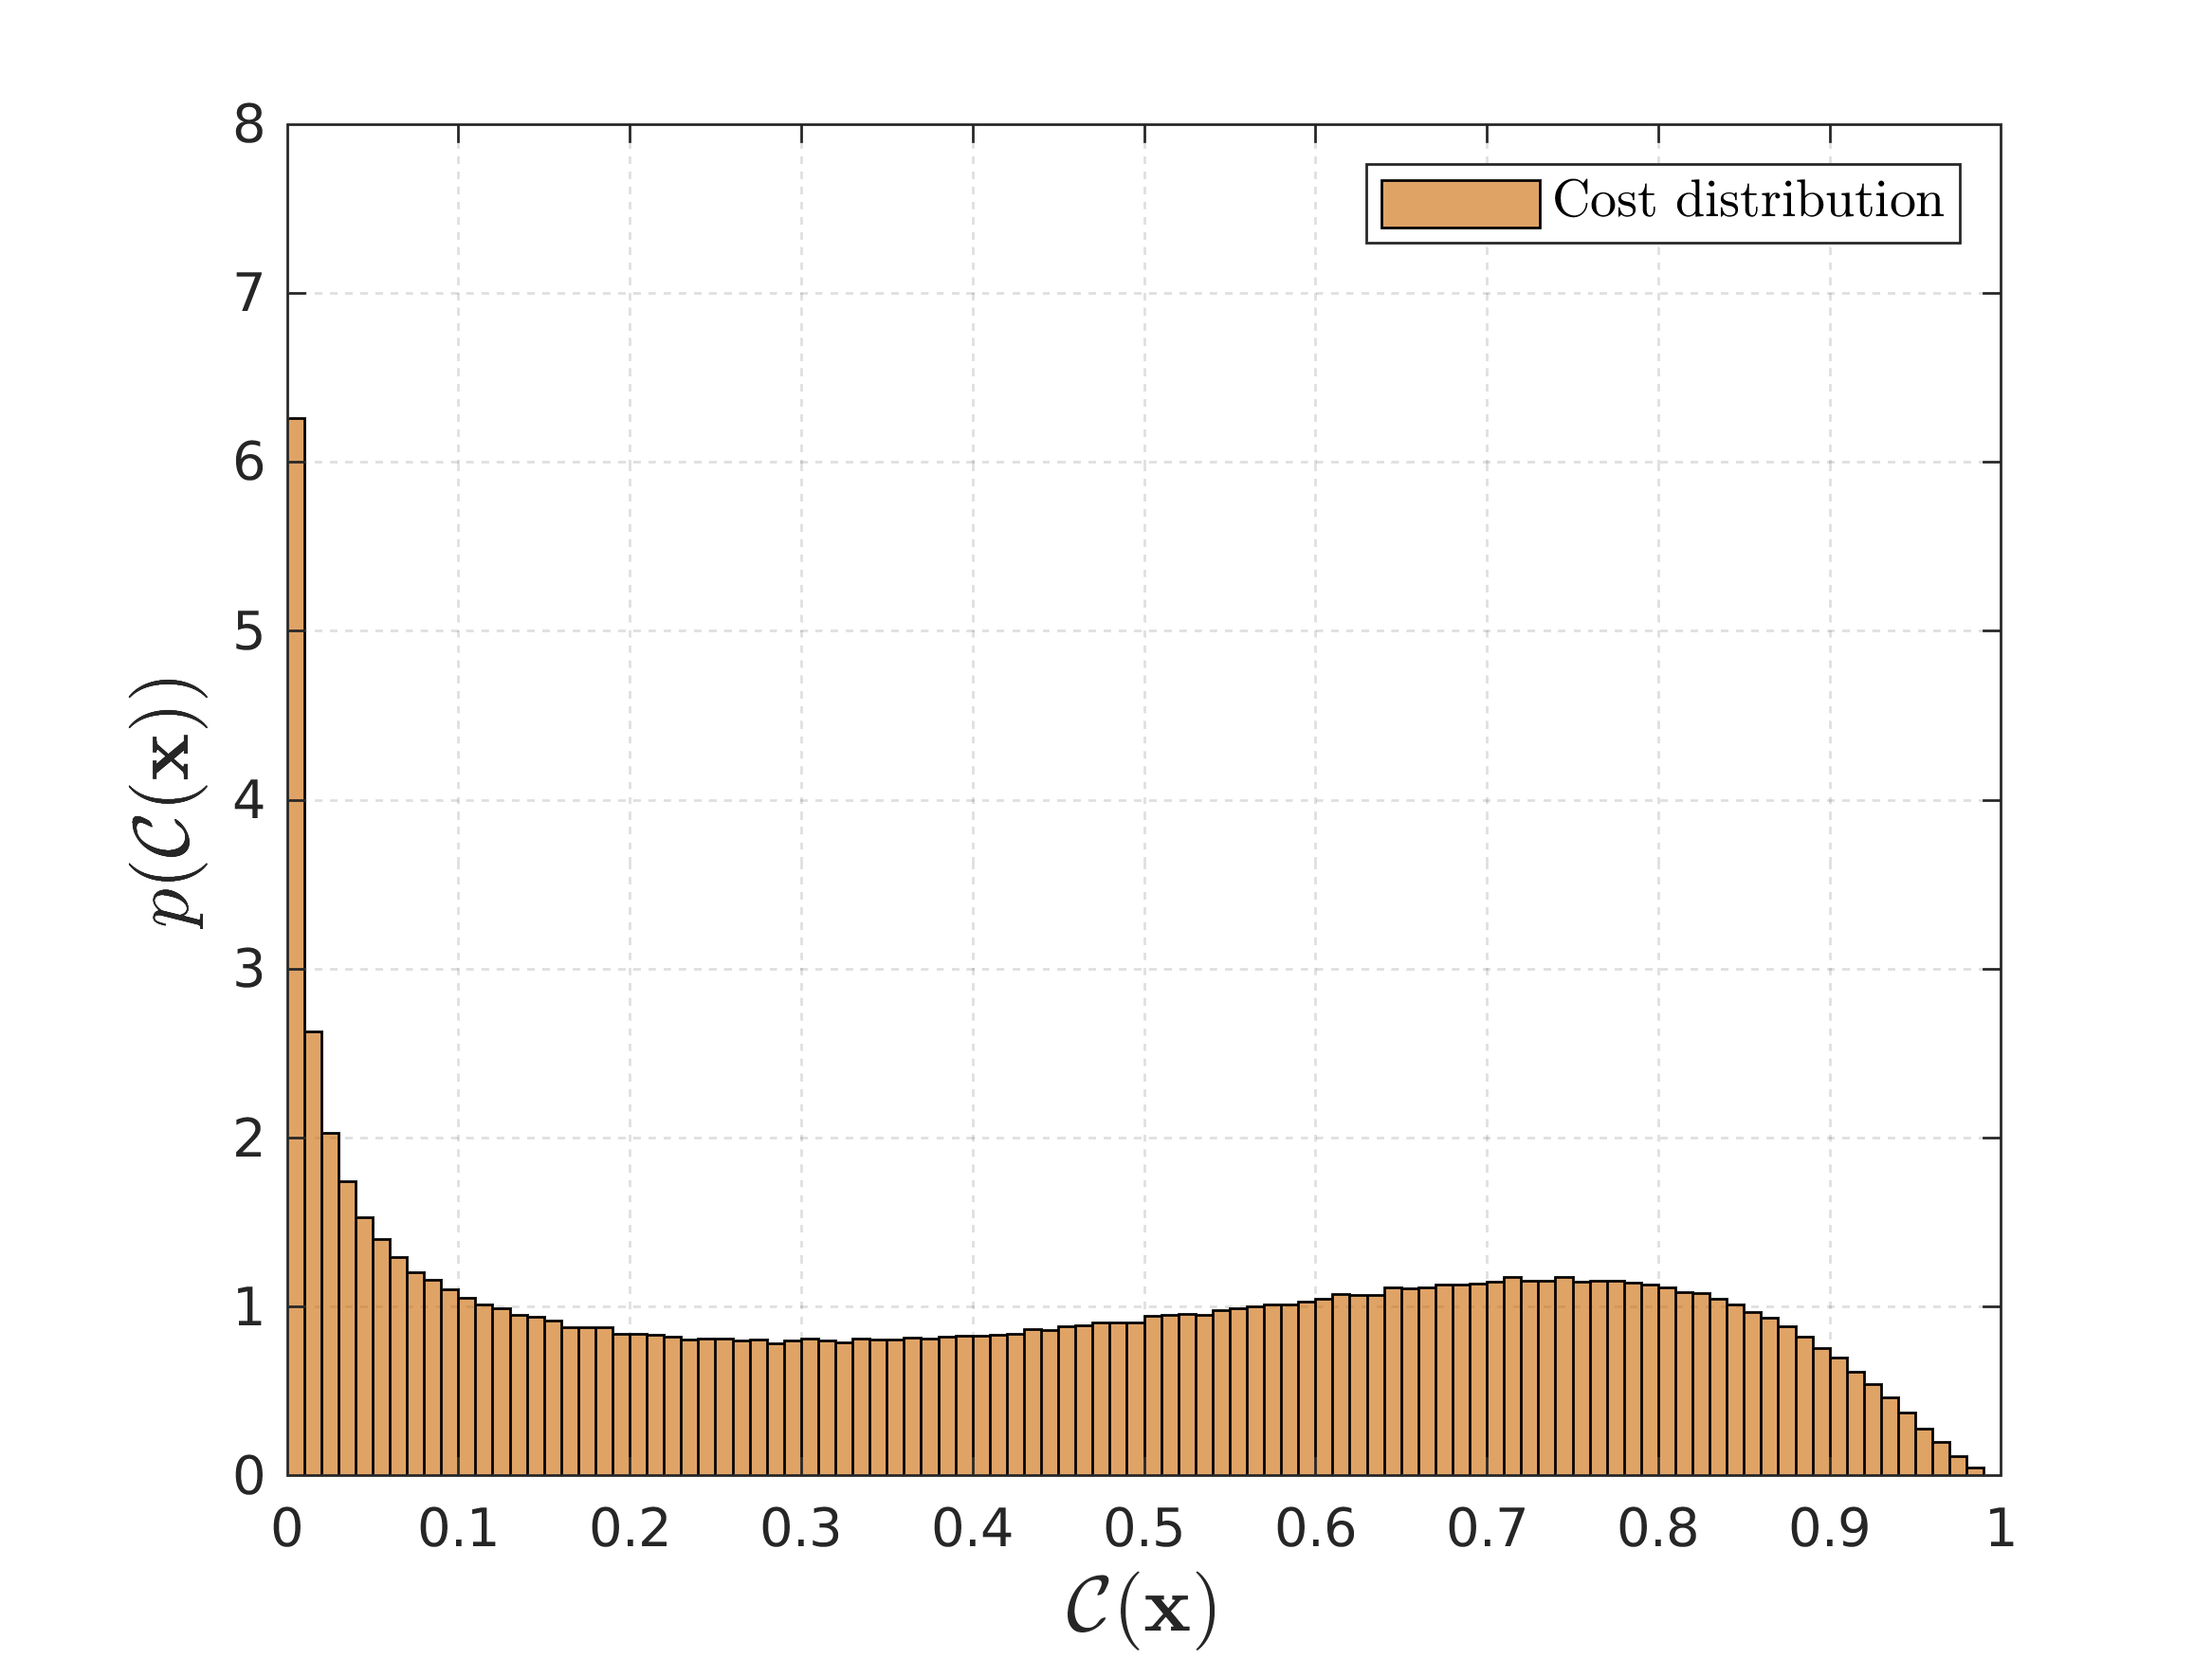
\includegraphics[height=0.25\textheight,width=1\textwidth]{Chapter3/Figures/trans_cost_hist_4.png} 
    \caption{Distribution over costs after 9 transitions} 
    \label{Fig:Re-hist-cost-4} 
  \end{subfigure} 
\caption[Evolution of state and cost distributions]{The evolution of state and cost distributions with increasing numbers of steps through the transition function.}
\label{Fig:Re-evolution-of-state-and-cost} 
\end{figure}

\subsection{A Decomposition of Transition Function Uncertainty}
A toy data set is used to illustrate the Monte-Carlo scheme for estimating the aleatoric and epistemic uncertainties present in the cost $\mathbb{C}(\mathbf{x})$ under policy $\pi$. Similar to the previous experiment, a 1-dimensional transition function is used and an explicit policy is not defined. This is viewed as if there is only one action available for selection and the agent selects that action at each opportunity. In this experiment, the agent begins by observing 4 transition data points. It then progressively observes more data a single point at a time up to a total of 50 data points. At each observation, the trigonometric basis function model is used to form a belief over the transition dynamics of the environment. Fig. \ref{Fig:Re-pred-4-points}-\ref{Fig:Re-pred-50-points} shows the predictive distribution over the transition data and 4 functions sampled from the posterior distribution over the weights after 4, 25 and 50 observations, respectively. For this, the lengthscale of the spectral points was purposely set to a large value to over fit the data as can be seen in Fig. \ref{Fig:Re-pred-4-points}. This was done for two reasons: to artificially induce more epistemic uncertainty into the model and to be more representative of a higher dimensional space where the observation of a single data point provides the model with more information than in the 1-dimensional case. The figures show that as more data is observed, the model becomes increasingly confident about the parameters and as a consequence the posterior distribution narrows. 

Each time a new data point is observed, Monte-Carlo trajectory roll outs are performed through the model using the one-step predictions following the procedure described in Sec. \ref{S:monte-carlo-estimate} for ($M=100,\: N=100,\: T=100$). The uncertainty 

 using Eq. \ref{S:monte-carlo-estimate}

% In model-based reinforcement learning, as the agent interacts with an environment it imparts actions and observes transitions through the state-space. It then uses these data to build a belief about the world which it can search to plan future interactions. The uncertainty present in the  transitions through the environment dynamics under a particular policy $\pi$ creates uncertainty in the cost, of which there are both aleatoric and epistemic components. A toy dataset is used here to illustrate how the Monte-Carlo scheme in 


% In complex problems with large state-spaces only limited parts of the space are relevant to the learning objective and the agent must make decisions 

% and uses this model to search for its next policy. 
% to plan its next policy to maximise information retrieval in the next trial. As more data are observed, these beliefs are refined and the agent becomes increasingly confident about its understanding. In complex problems with large state-spaces only limited parts of the space are relevant to the learning objective and the agent must decisions 


% extract relevant information from the data to make informed decision about where to explore. 


% On it's path through the state space, the agent encounters both epist

% This can be illustrated with a 1-dimensional toy data set 
% represents a policy to explore the whole space
\begin{figure}[htp!]    
  \begin{subfigure}[b]{0.95\linewidth}
    \centering
    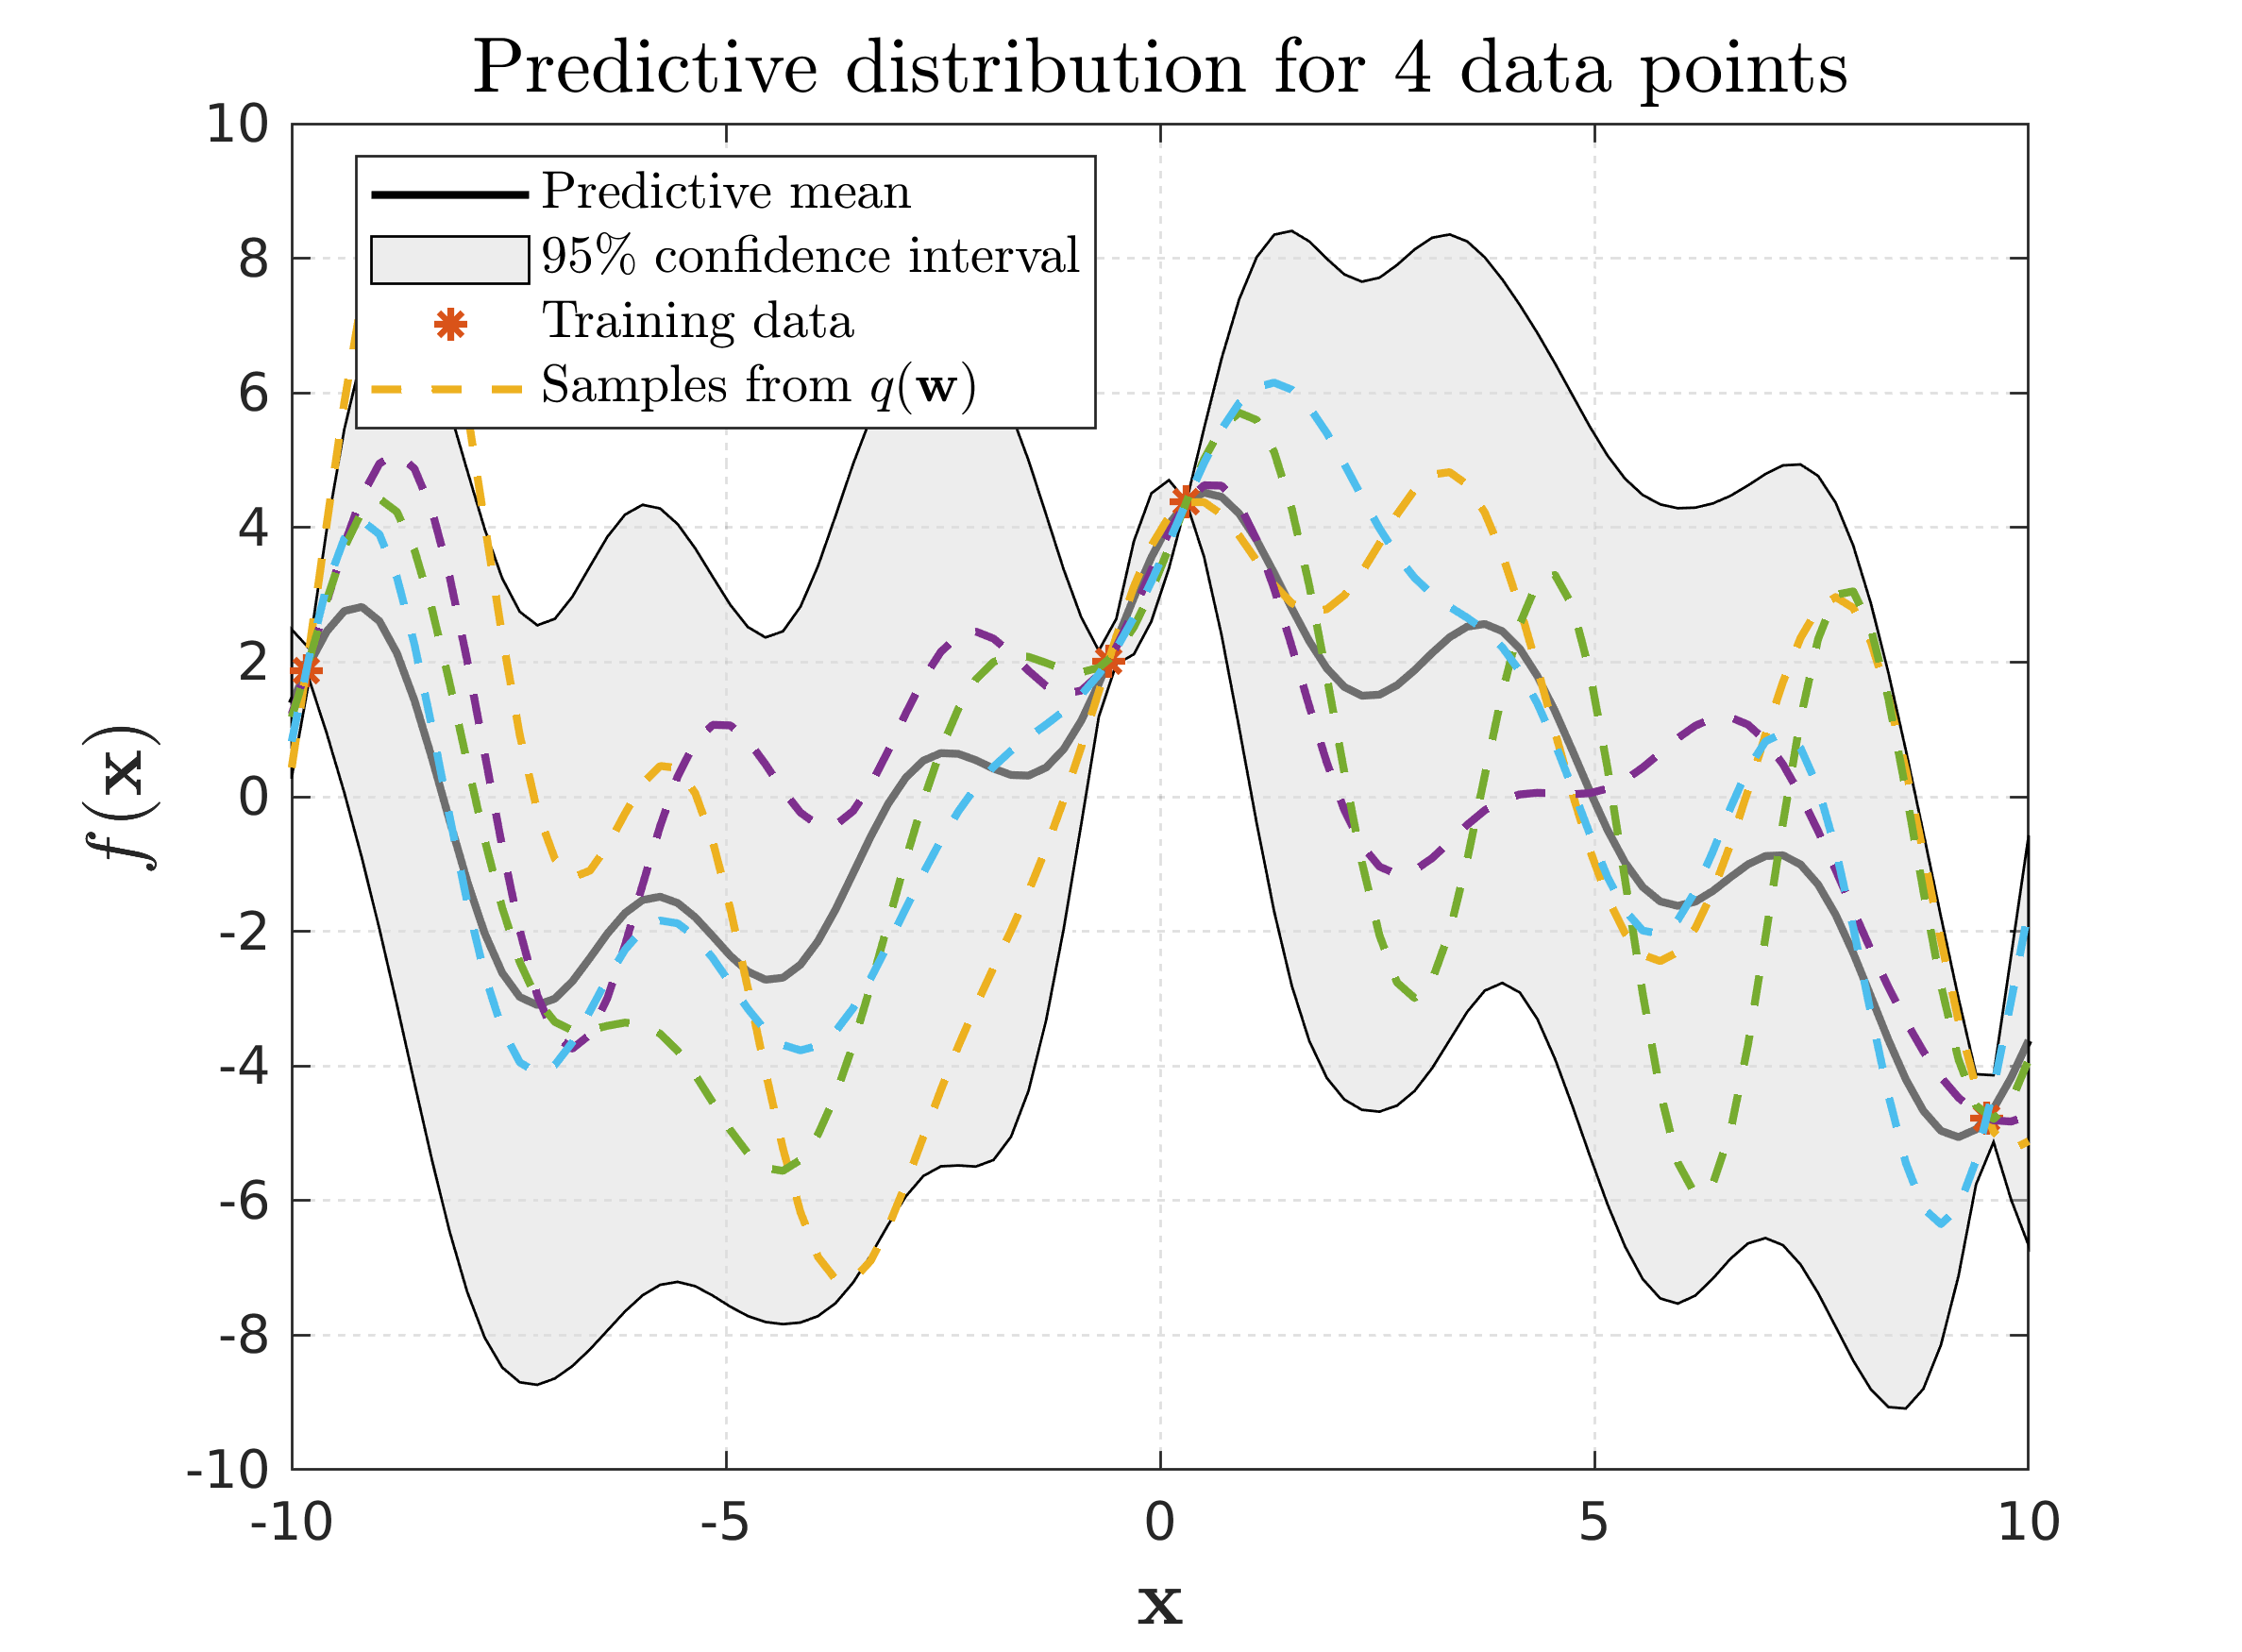
\includegraphics[trim={0 0.18cm 0 0.70cm},clip,height=0.27\textheight,width=0.75\textwidth]{Chapter3/Figures/func_uncertainty_1.png} 
    \caption{Predictive distribution for 4 data points} 
    \label{Fig:Re-pred-4-points} 
  \end{subfigure}

  \begin{subfigure}[b]{0.95\linewidth}
    \centering
    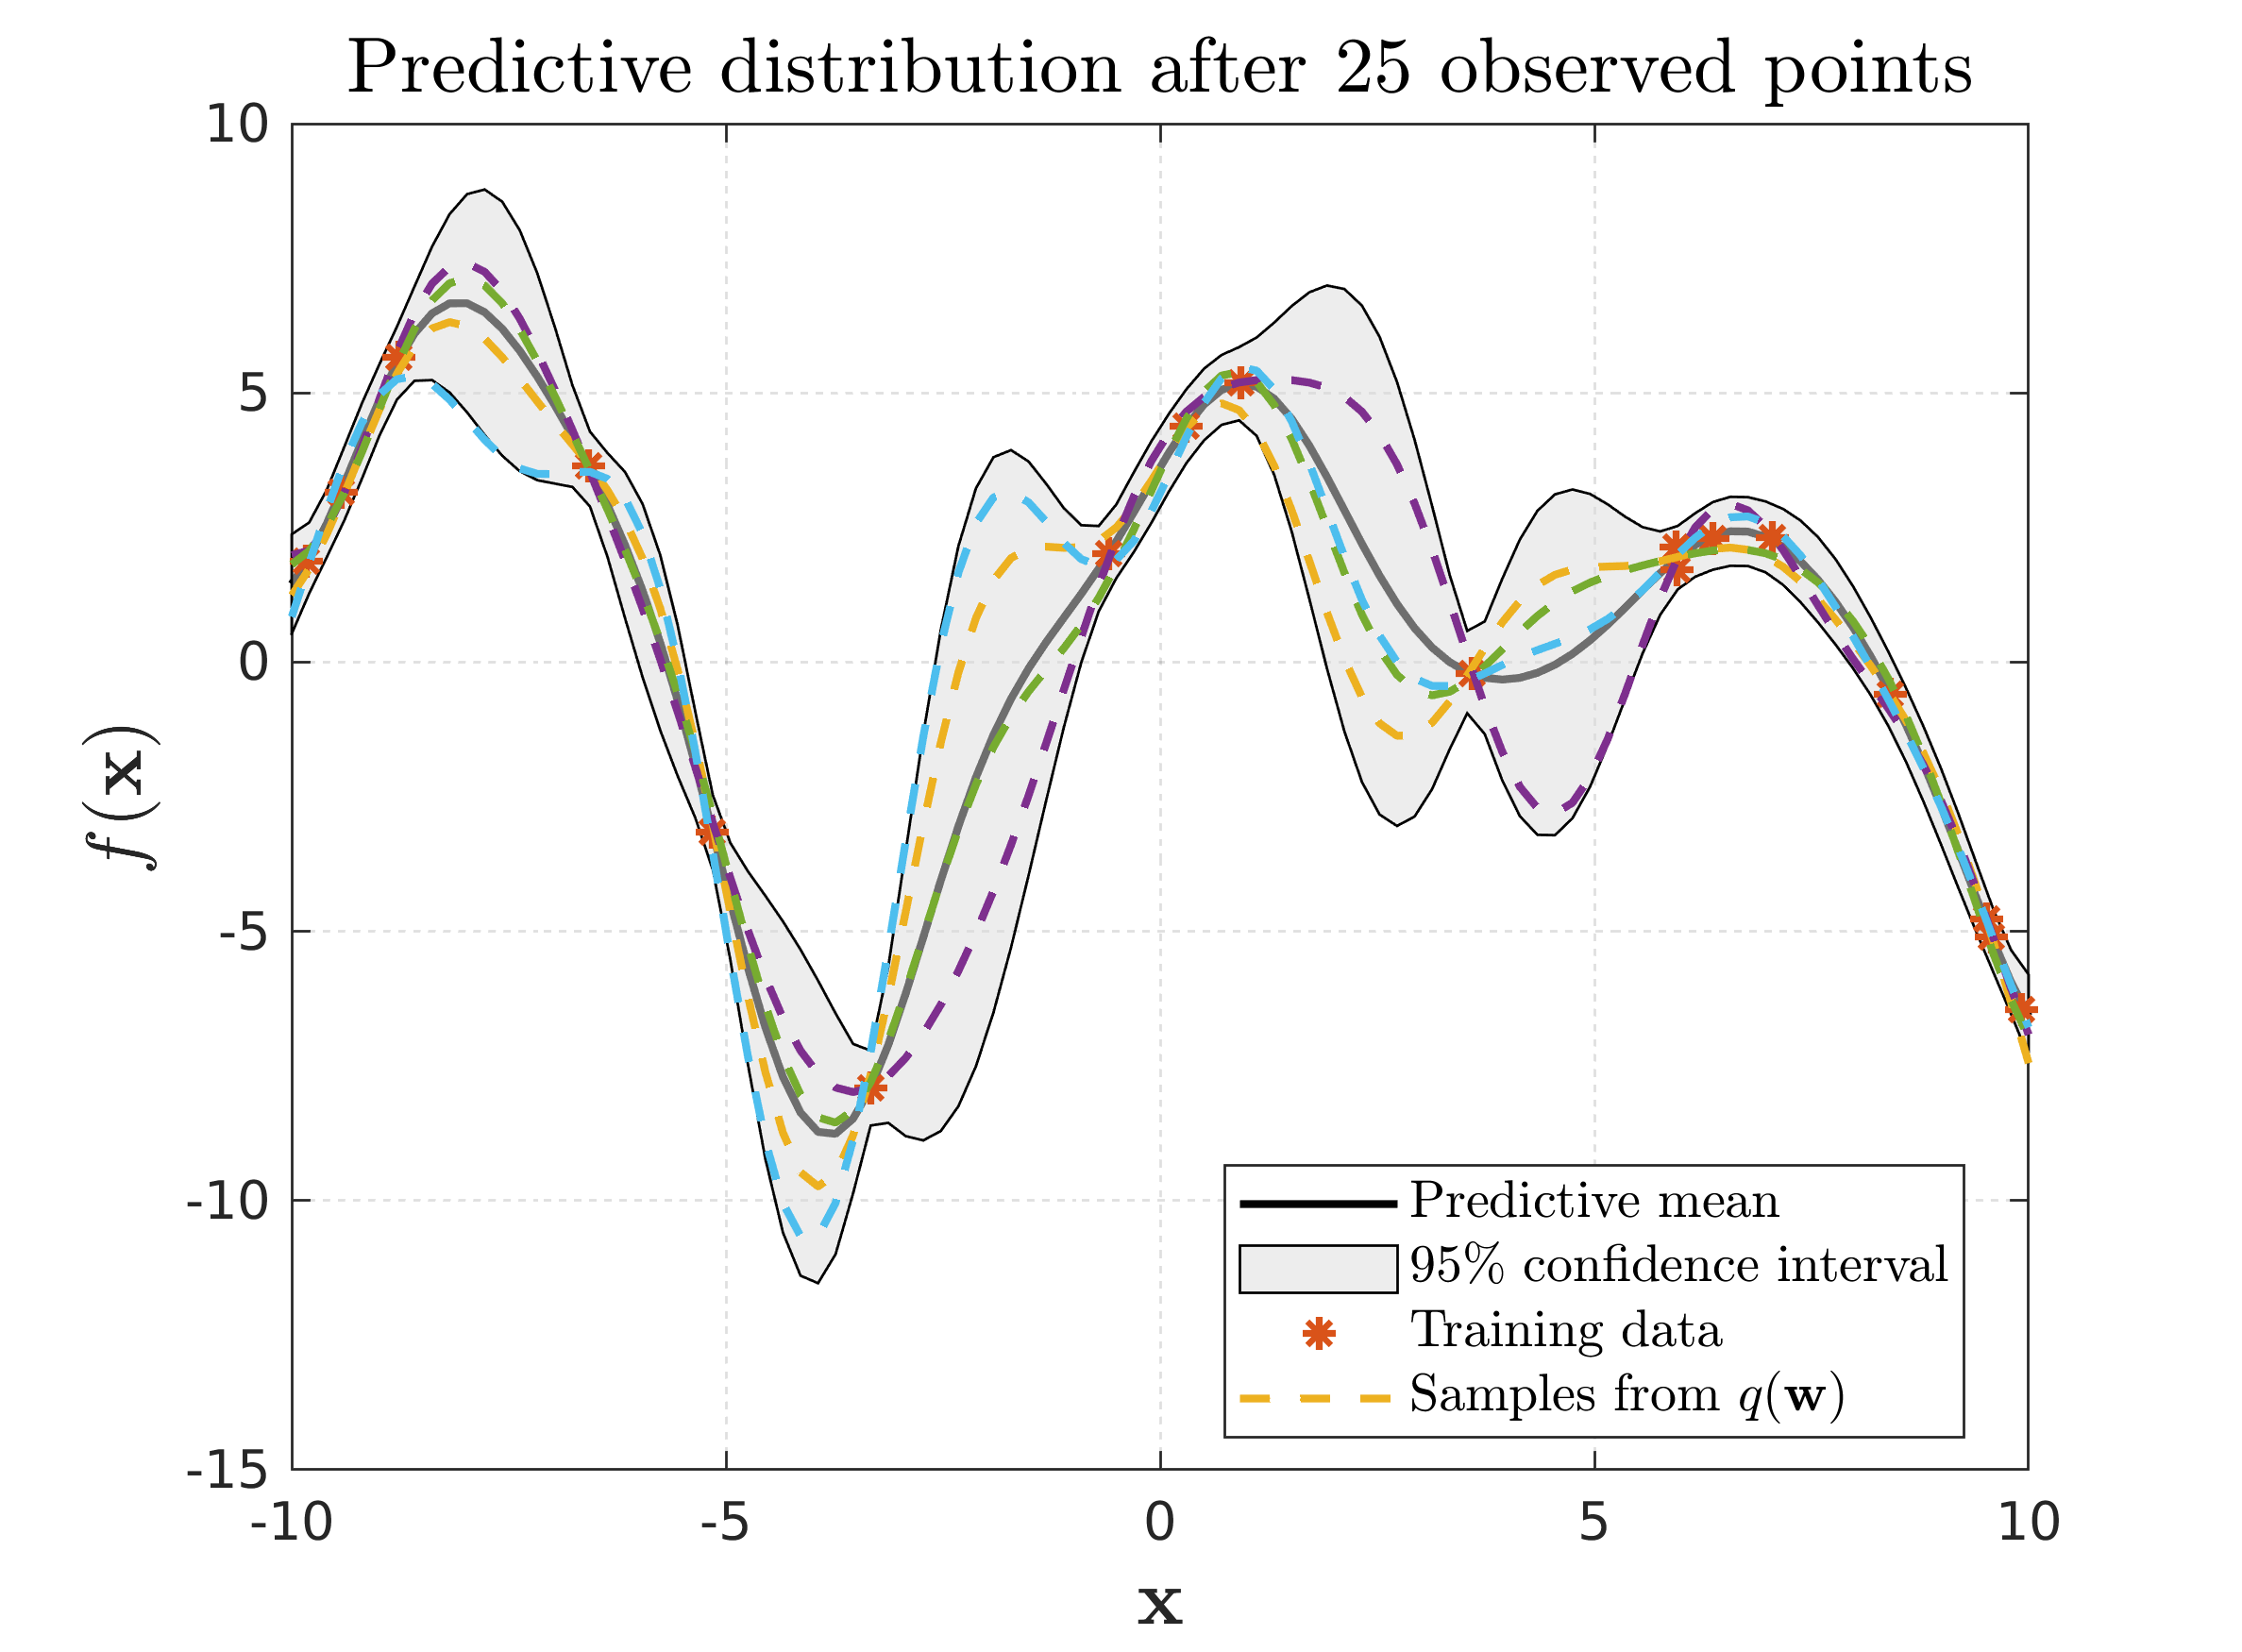
\includegraphics[trim={0 0.18cm 0 0.70cm},clip,height=0.27\textheight,width=0.75\textwidth]{Chapter3/Figures/func_uncertainty_2.png} 
    \caption{Predictive distribution after 25 data points} 
    \label{Fig:Re-pred-25-points}
  \end{subfigure}
  
  \begin{subfigure}[b]{0.95\linewidth}
    \centering
    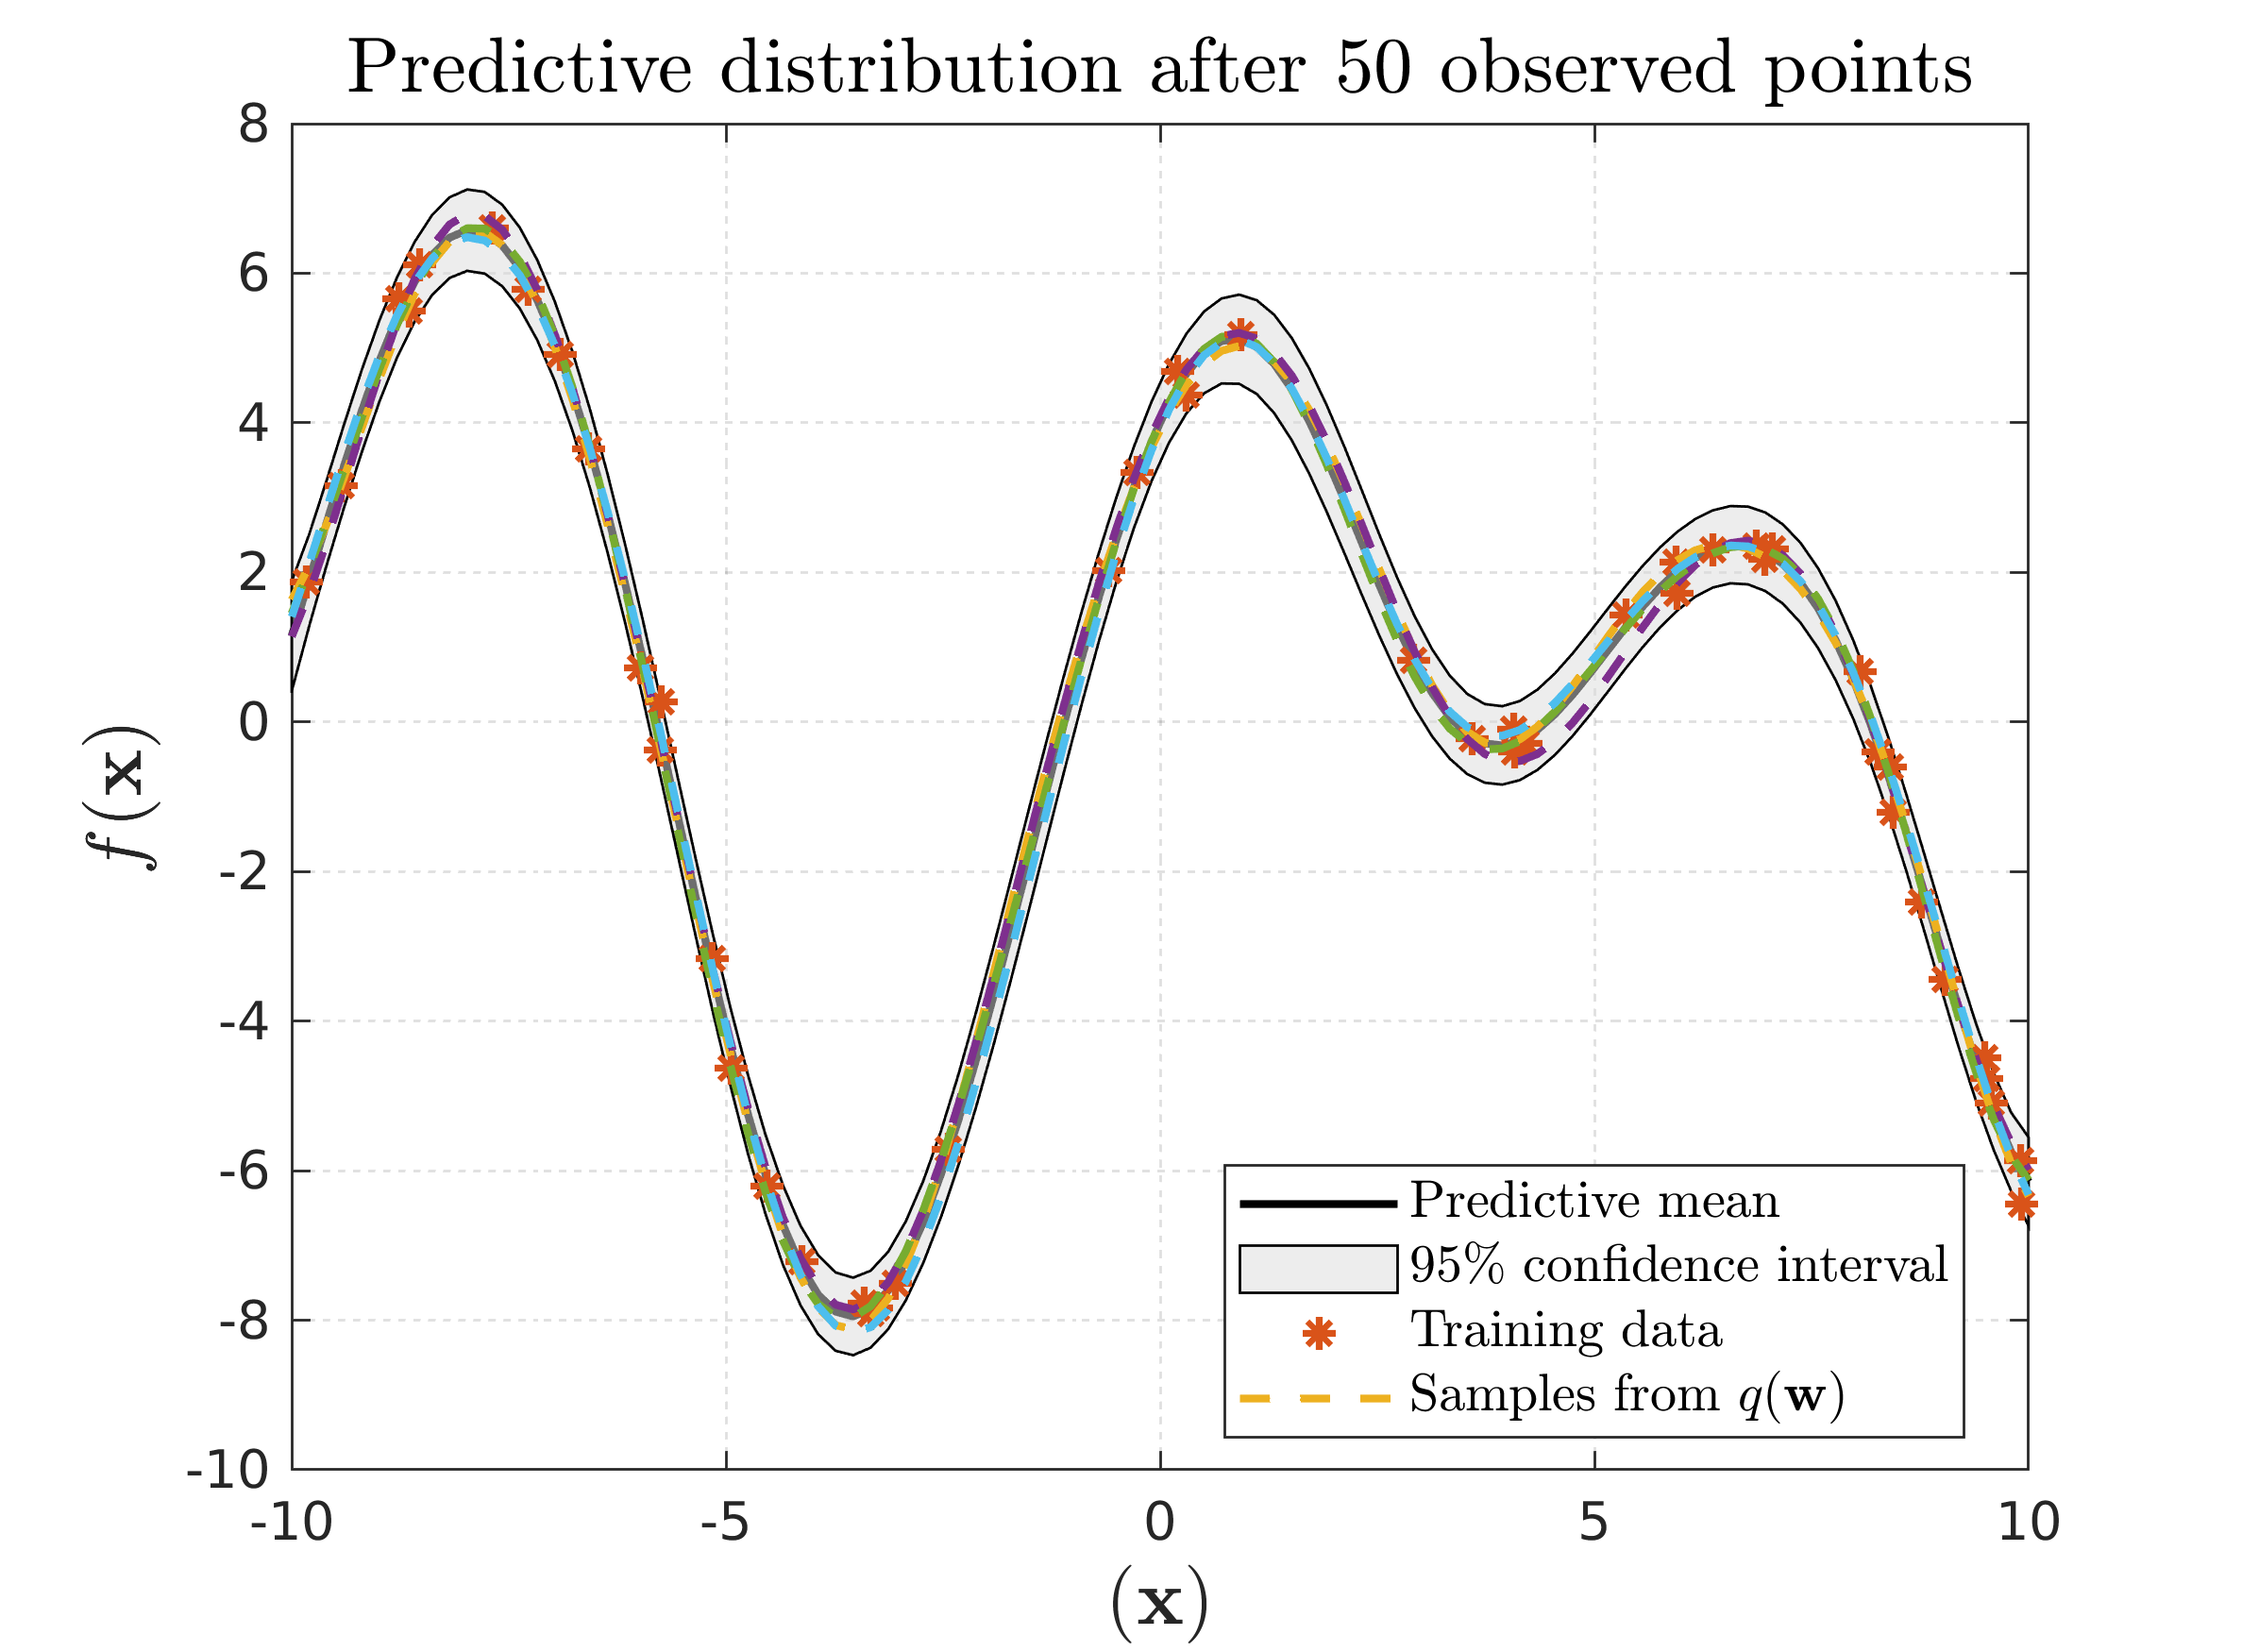
\includegraphics[trim={0 0.1cm 0 0.70cm},clip,height=0.27\textheight,width=0.75\textwidth]{Chapter3/Figures/func_uncertainty_3.png} 
    \caption{Predictive distribution after 50 data points} 
    \label{Fig:Re-pred-50-points}
  \end{subfigure}
 
\caption[Reduction in epistemic uncertainty with added data]{: Fig \ref{Fig:Re-pred-4-points} - \ref{Fig:Re-pred-50-points} show the predictive distribution over the data and samples from the posterior after 4, 25 and 50 observed data points. The lengthscale of the spectral points is purposely set to a high value to over fit the data and imitate high dimensional space. As more data is observed the model becomes increasingly confident about the parameter values and as a consequence the posterior distribution narrows.}
\label{Fig:Re-predictive-fit-to-varying-number-of-datapoints} 
\end{figure}

\begin{figure}[htp!]
\centering    
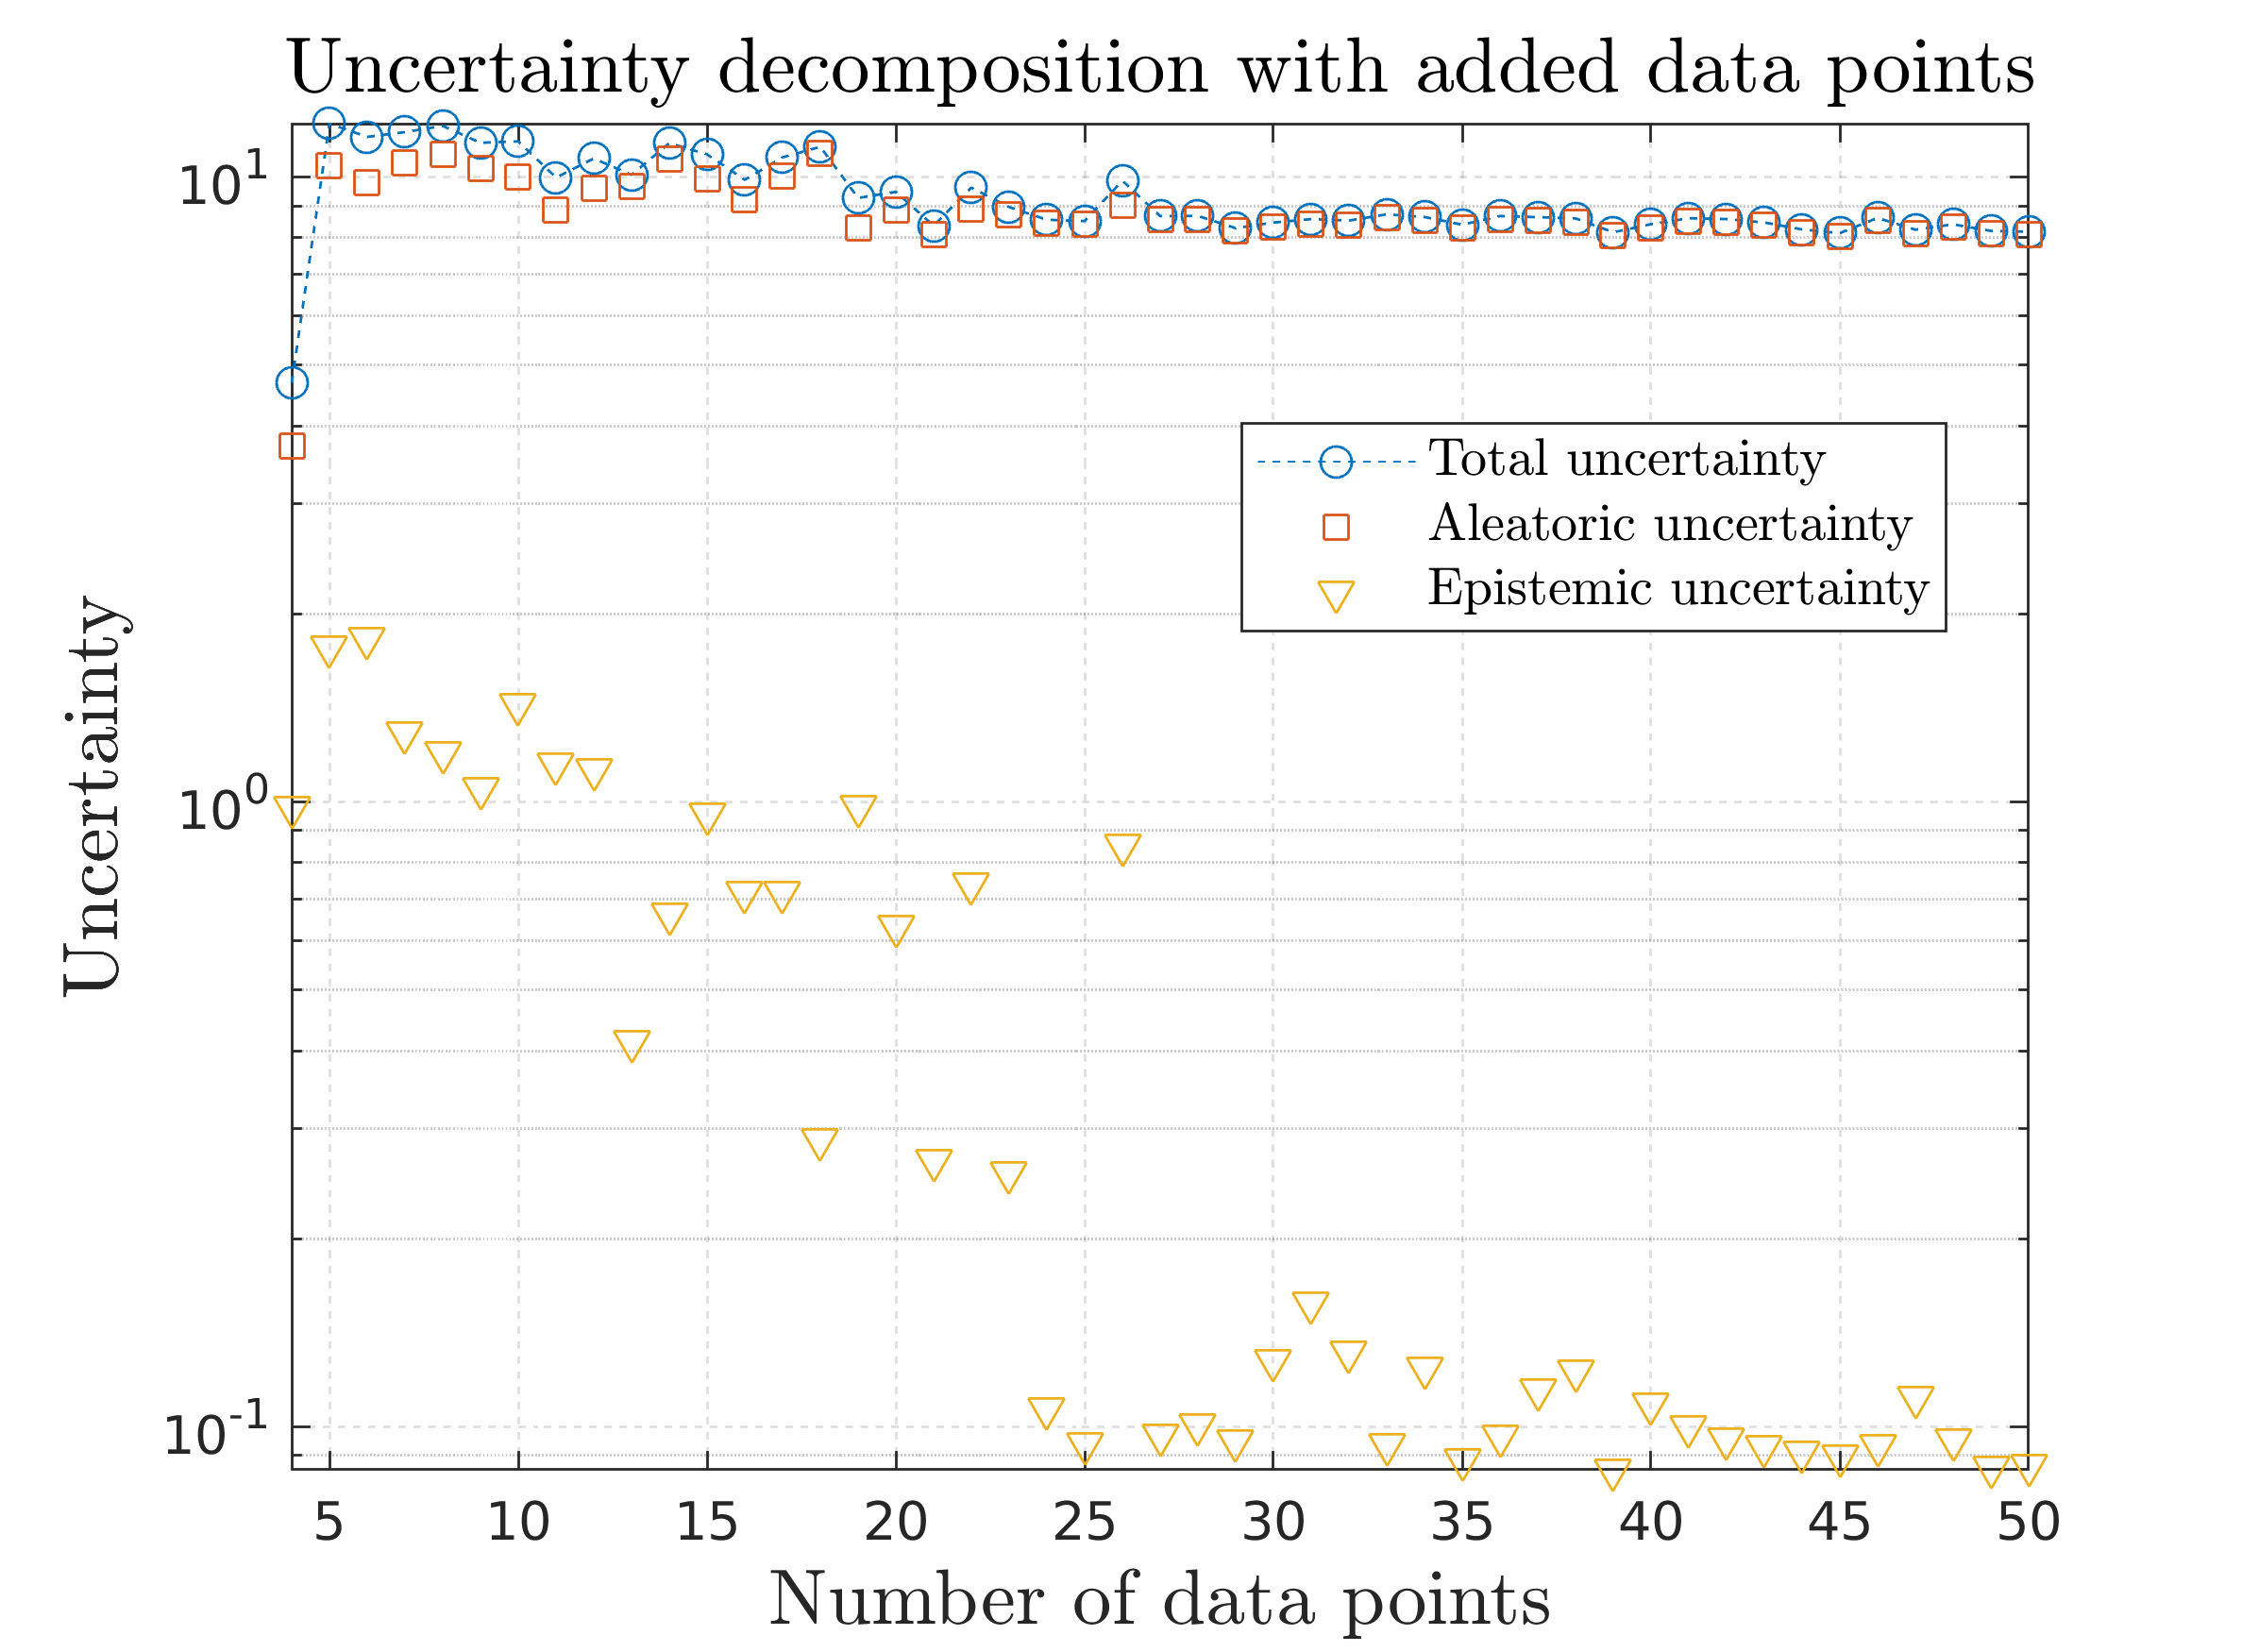
\includegraphics[width=1\textwidth]{Chapter3/Figures/func_uncertainty_4.png}
\caption[Uncertainty decomposition showing reduction in epistemic uncertainty with increasing number of data points]{Relating to Fig. \ref{Fig:Re-predictive-fit-to-varying-number-of-datapoints}. Trajectory roll outs were performed through the transition function each time a new data point was observed (from 4 to 50). For each roll out the uncertainty in the cost was decomposed. As more data is observed the model becomes increasingly confident about its parameters and consequently the epistemic uncertainty reduces due contraction of the posterior distribution.}
\label{Fig:Re-reduction-in-epsitemic-with-more-data}
\end{figure}


% \begin{figure}[H]    
%   \begin{subfigure}[b]{0.49\linewidth}
%     \centering
%     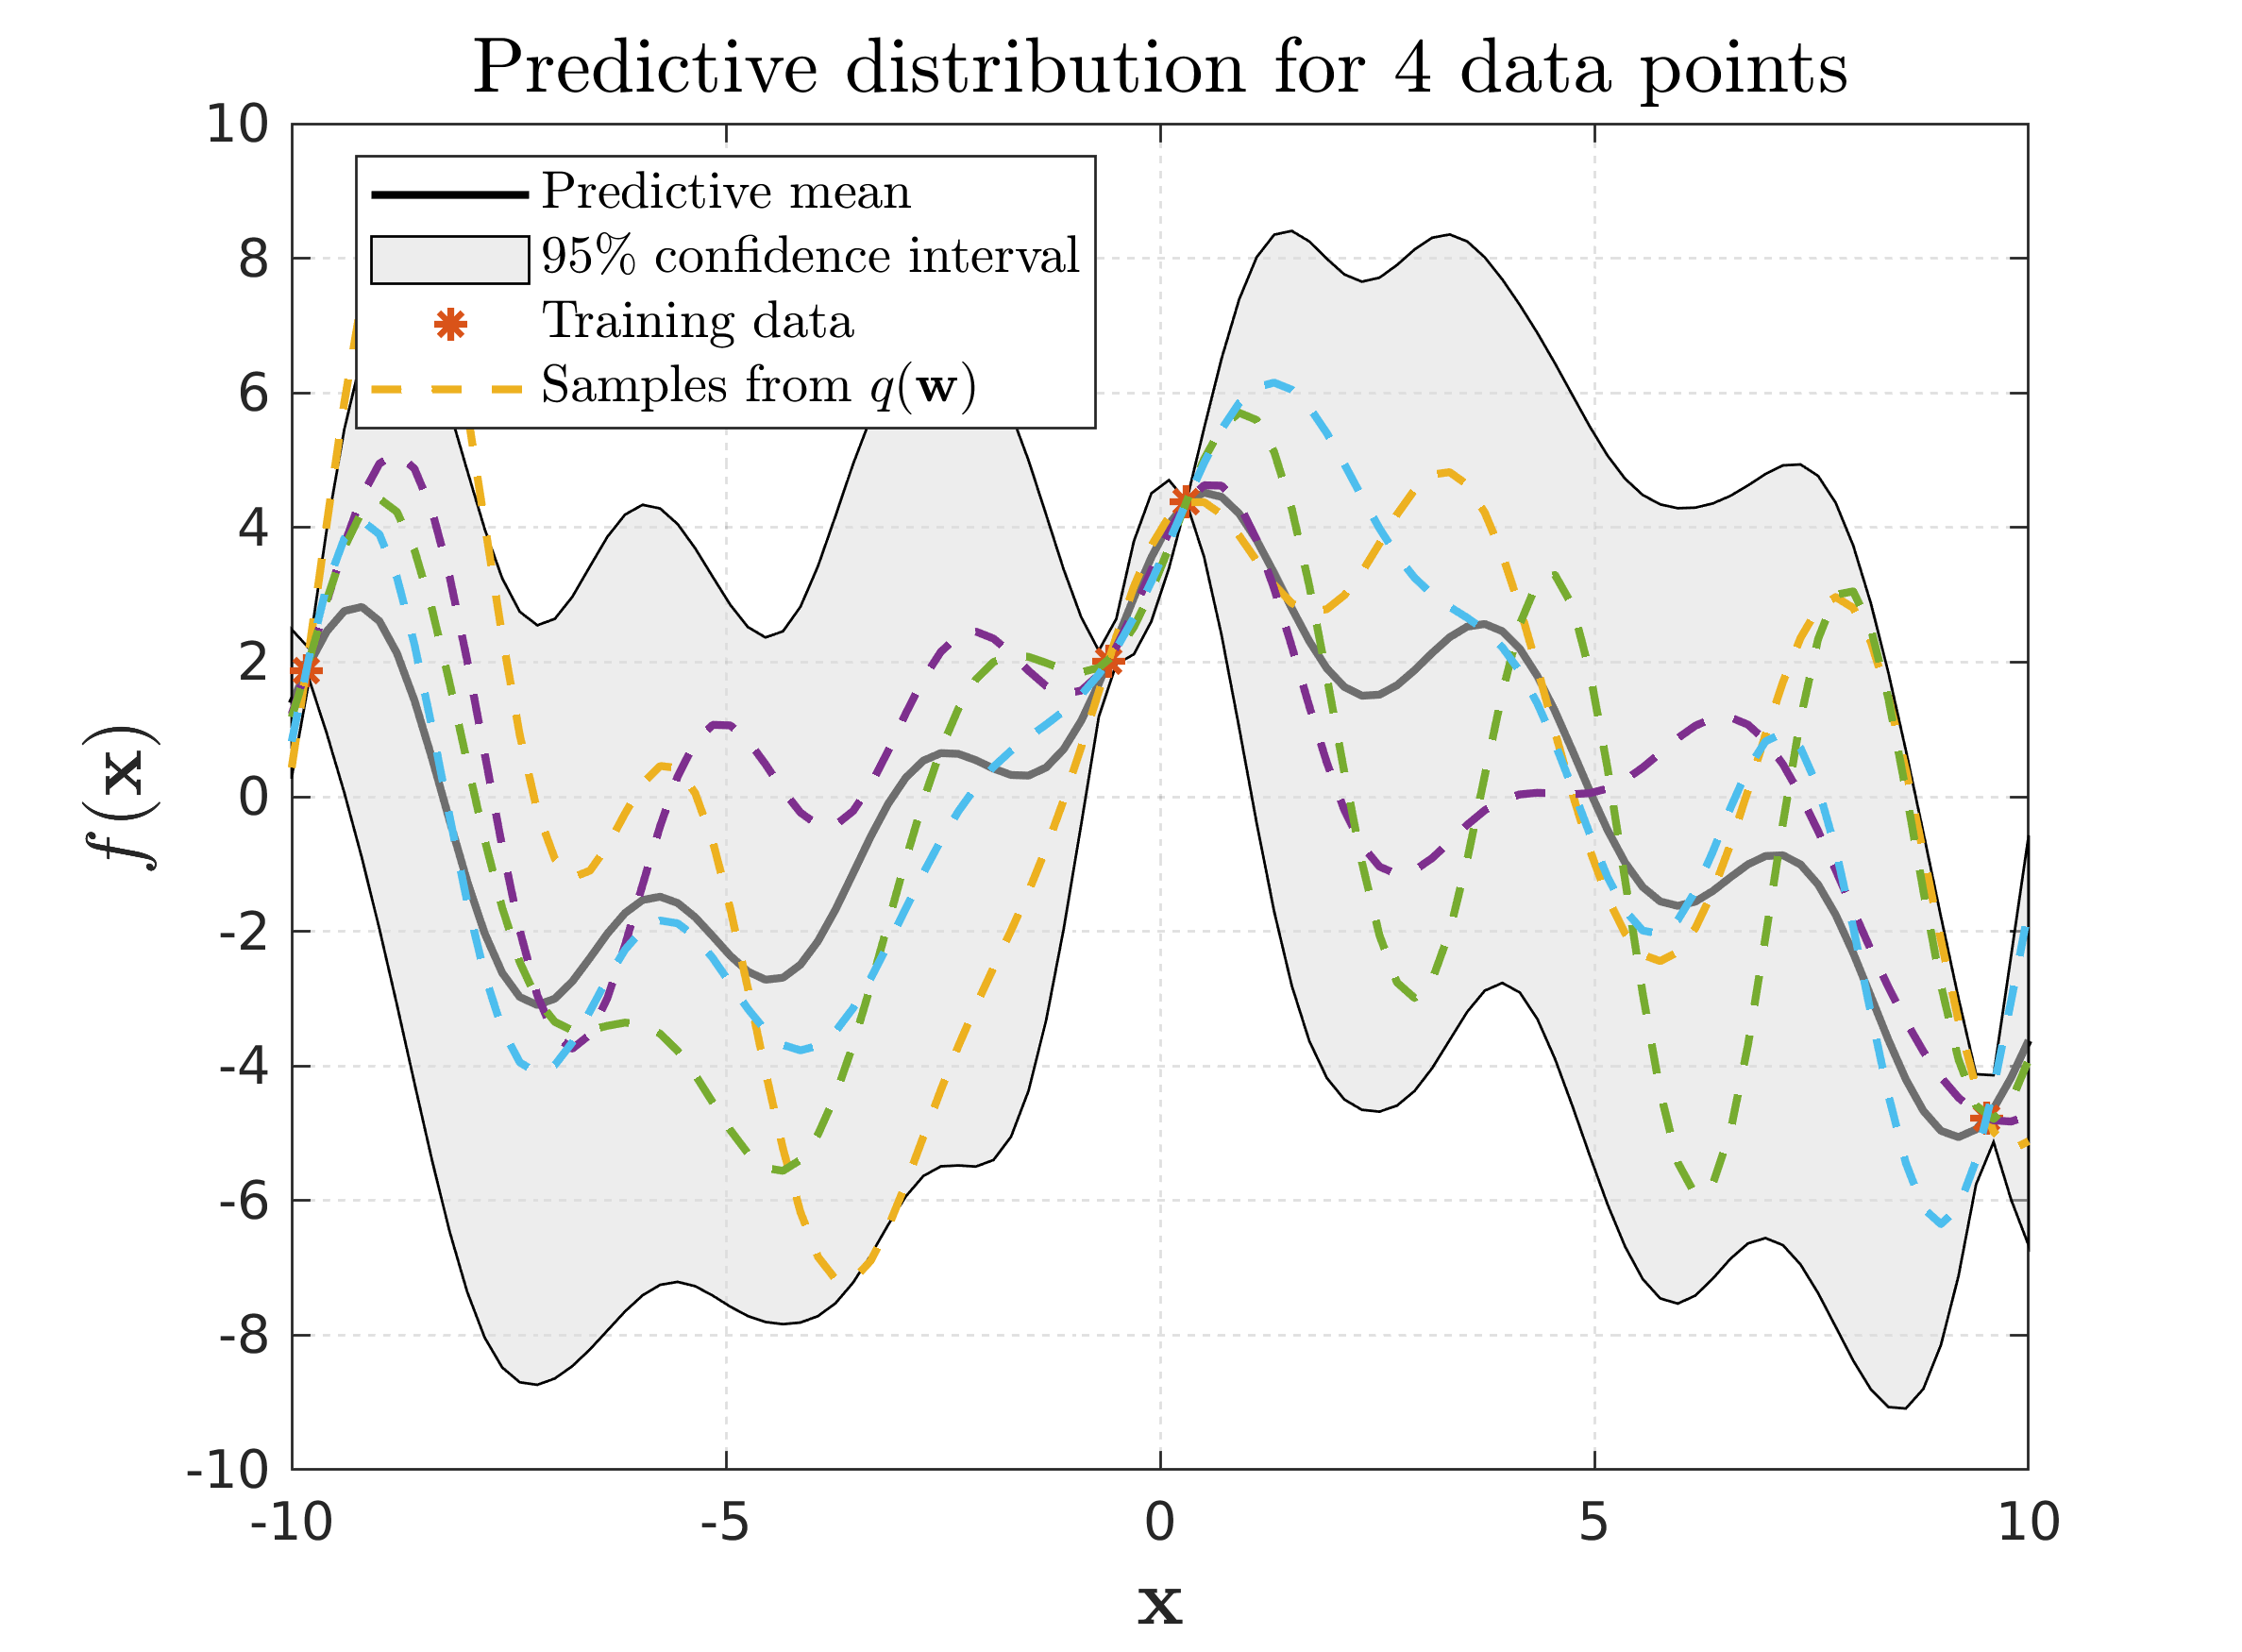
\includegraphics[height=0.25\textheight,width=1\textwidth]{Chapter3/Figures/func_uncertainty_1.png} 
%     \caption{Predictive distribution for 4 data points} 
%     \label{Fig:Re-pred-4-points} 
%   \end{subfigure} 
% %   \hspace{\fill}  %% maximize space between adjacent subfigures
%   \begin{subfigure}[b]{0.49\linewidth}
%     \centering
%     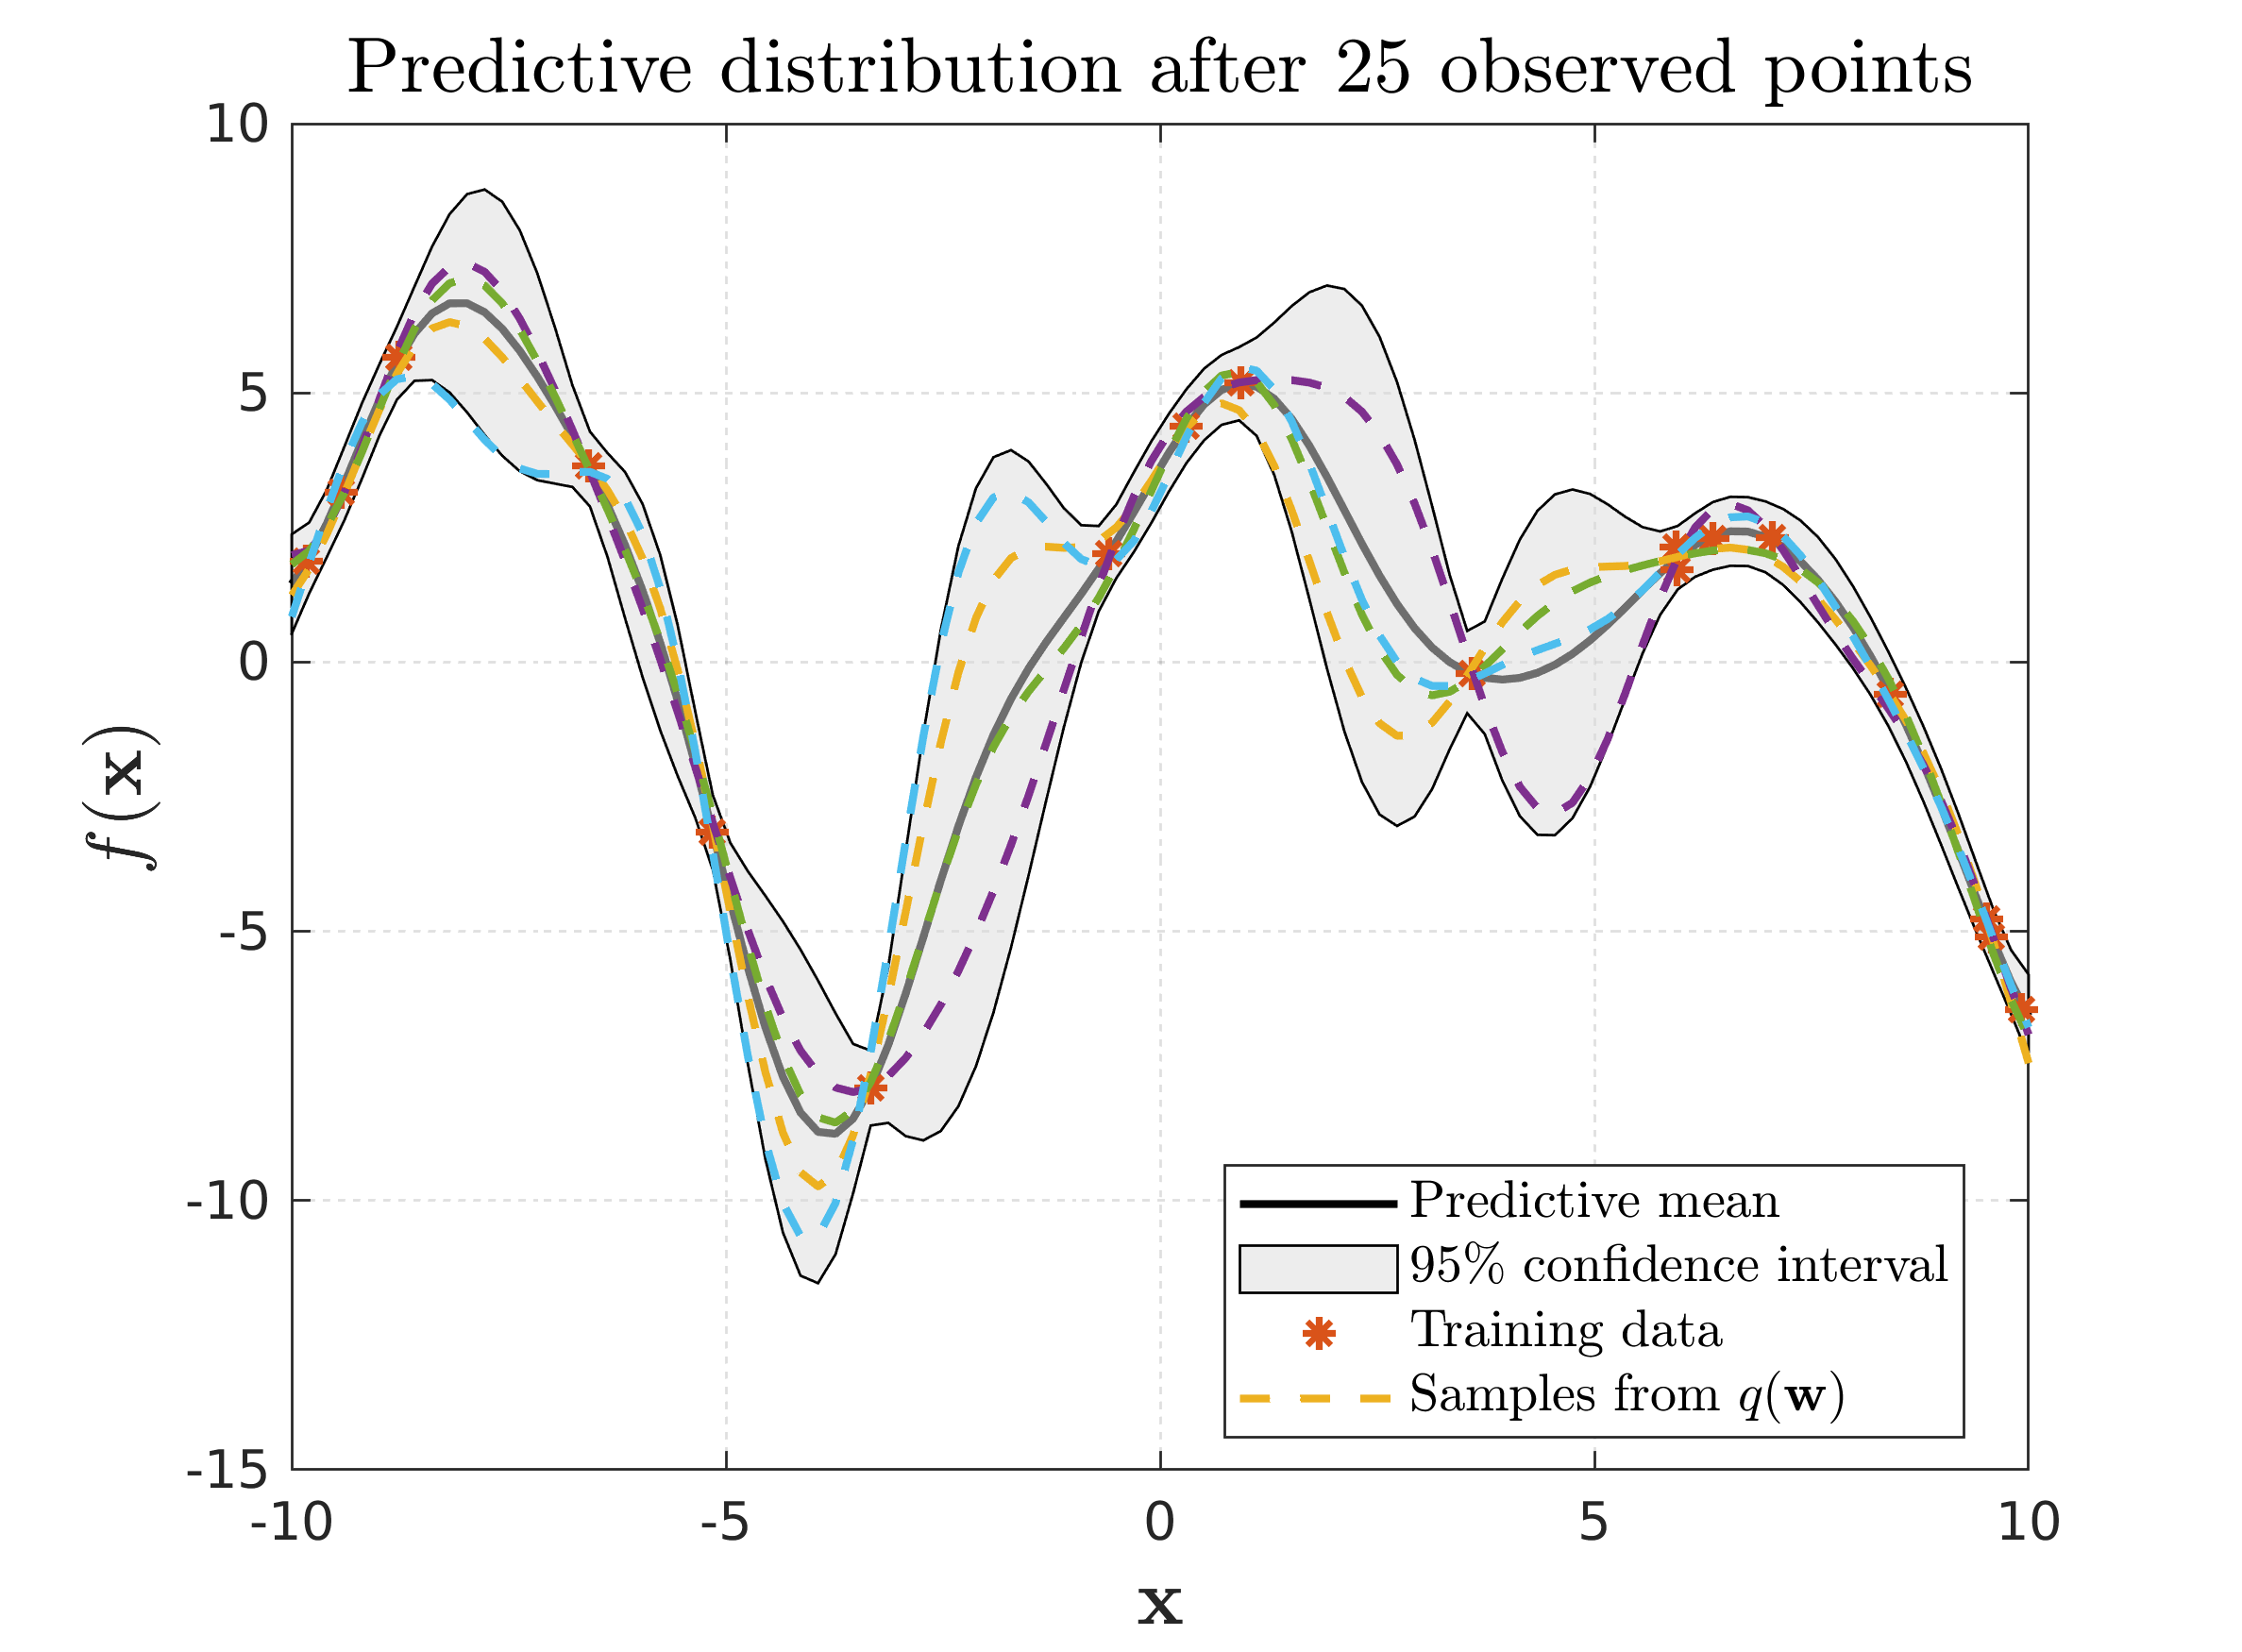
\includegraphics[height=0.25\textheight,width=1\textwidth]{Chapter3/Figures/func_uncertainty_2.png} 
%     \caption{Predictive distribution after 25 data points} 
%     \label{Fig:Re-pred-25-points}
%   \end{subfigure} 

%   \vspace{4ex}  %% extra vertical space
%   \begin{subfigure}[b]{0.49\linewidth}
%     \centering
%     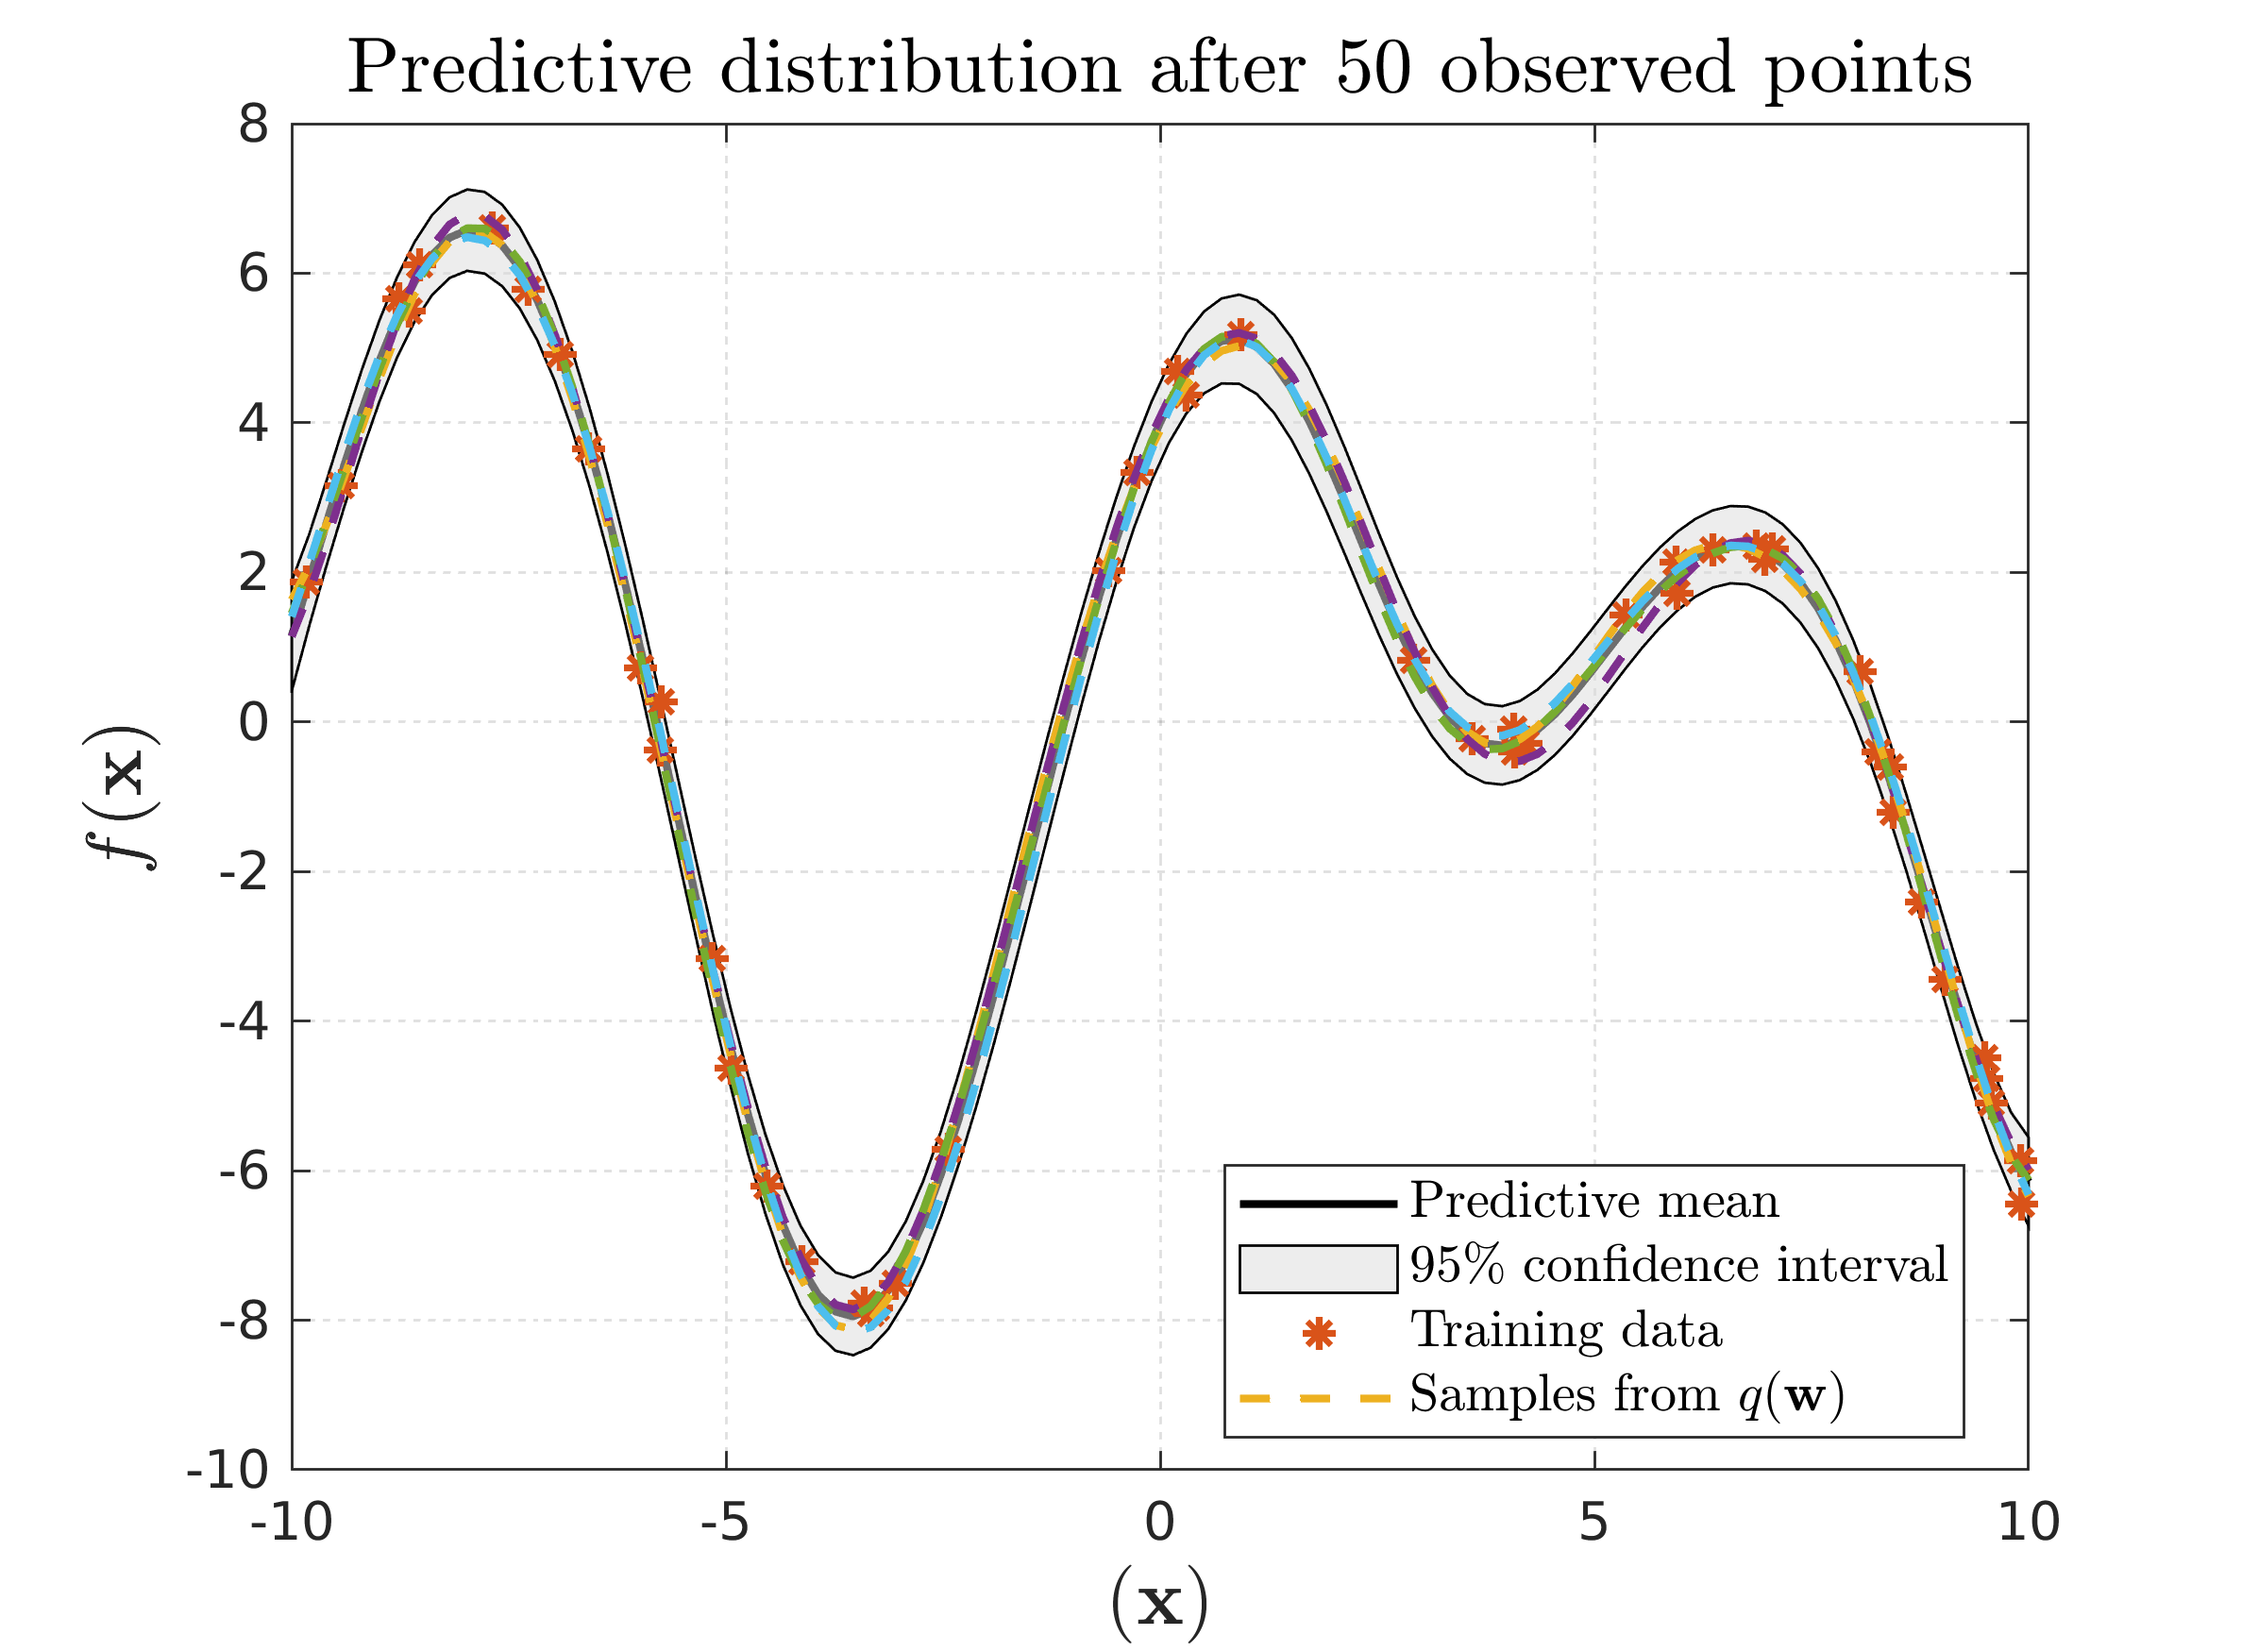
\includegraphics[height=0.25\textheight,width=0.95\textwidth]{Chapter3/Figures/func_uncertainty_3.png} 
%     \caption{Predictive distribution after 50 data points} 
%     \label{Fig:Re-pred-50-points}
%   \end{subfigure} 
% %   \hspace{\fill}
%   \begin{subfigure}[b]{0.49\linewidth}
%     \centering
%     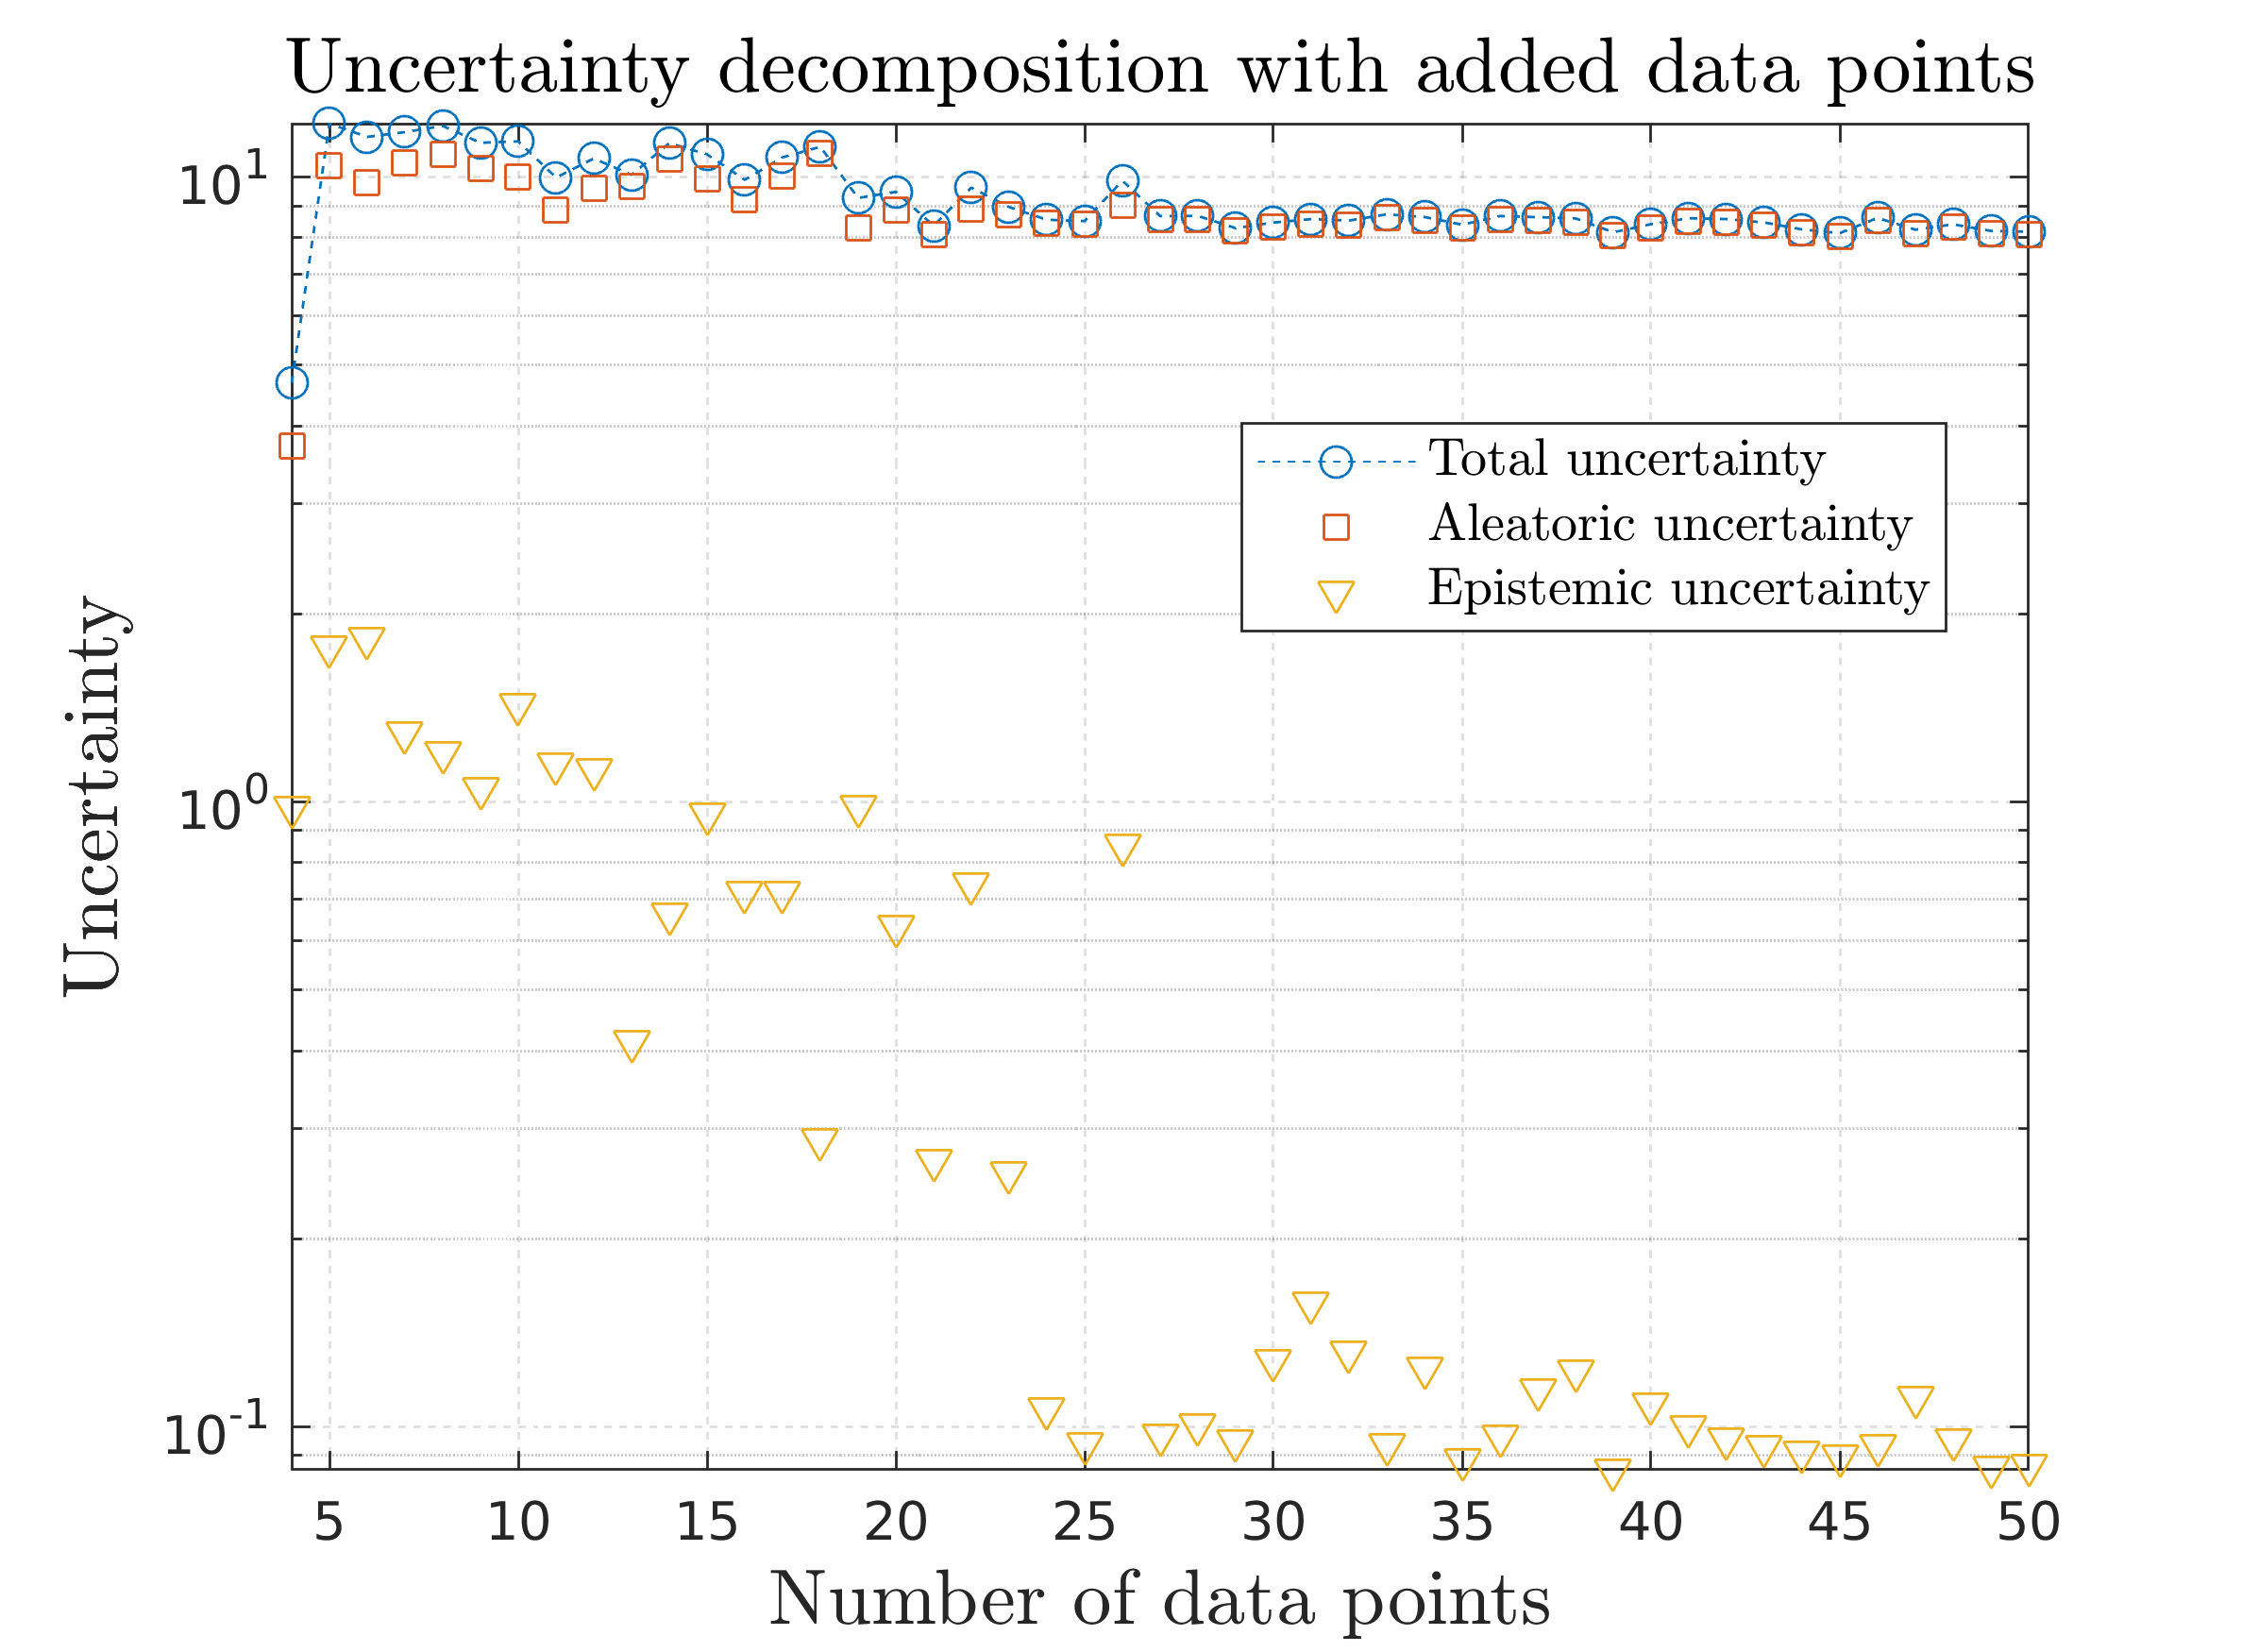
\includegraphics[height=0.25\textheight,width=1\textwidth]{Chapter3/Figures/func_uncertainty_4.png} 
%     \caption{Uncertainty decomposition with added data} 
%     \label{Fig:Re-function-uncertainty} 
%   \end{subfigure} 

% \caption[Reduction in epistemic uncertainty with added data]{: Fig \ref{Fig:Re-pred-4-points} - \ref{Fig:Re-pred-50-points} show the predictive distribution over the data after 4, 25 and 50 data points where the lengthscale of the spectral points purposely set to a high value to over fit the data and imitate high dimensional space. Trajectory rollouts are performed through the transition function for each new data point added and the cost calculated. Fig. \ref{Fig:Re-function-uncertainty} shows that as more data is observed the model becomes increasingly confident about its parameters and consequently the epistemic uncertainty reduces due contraction of the posterior distribution.}
% \label{} 
% \end{figure}



% \begin{landscape}
% \begin{figure}[H]    
%   \begin{subfigure}[b]{0.49\linewidth}
%     \centering
%     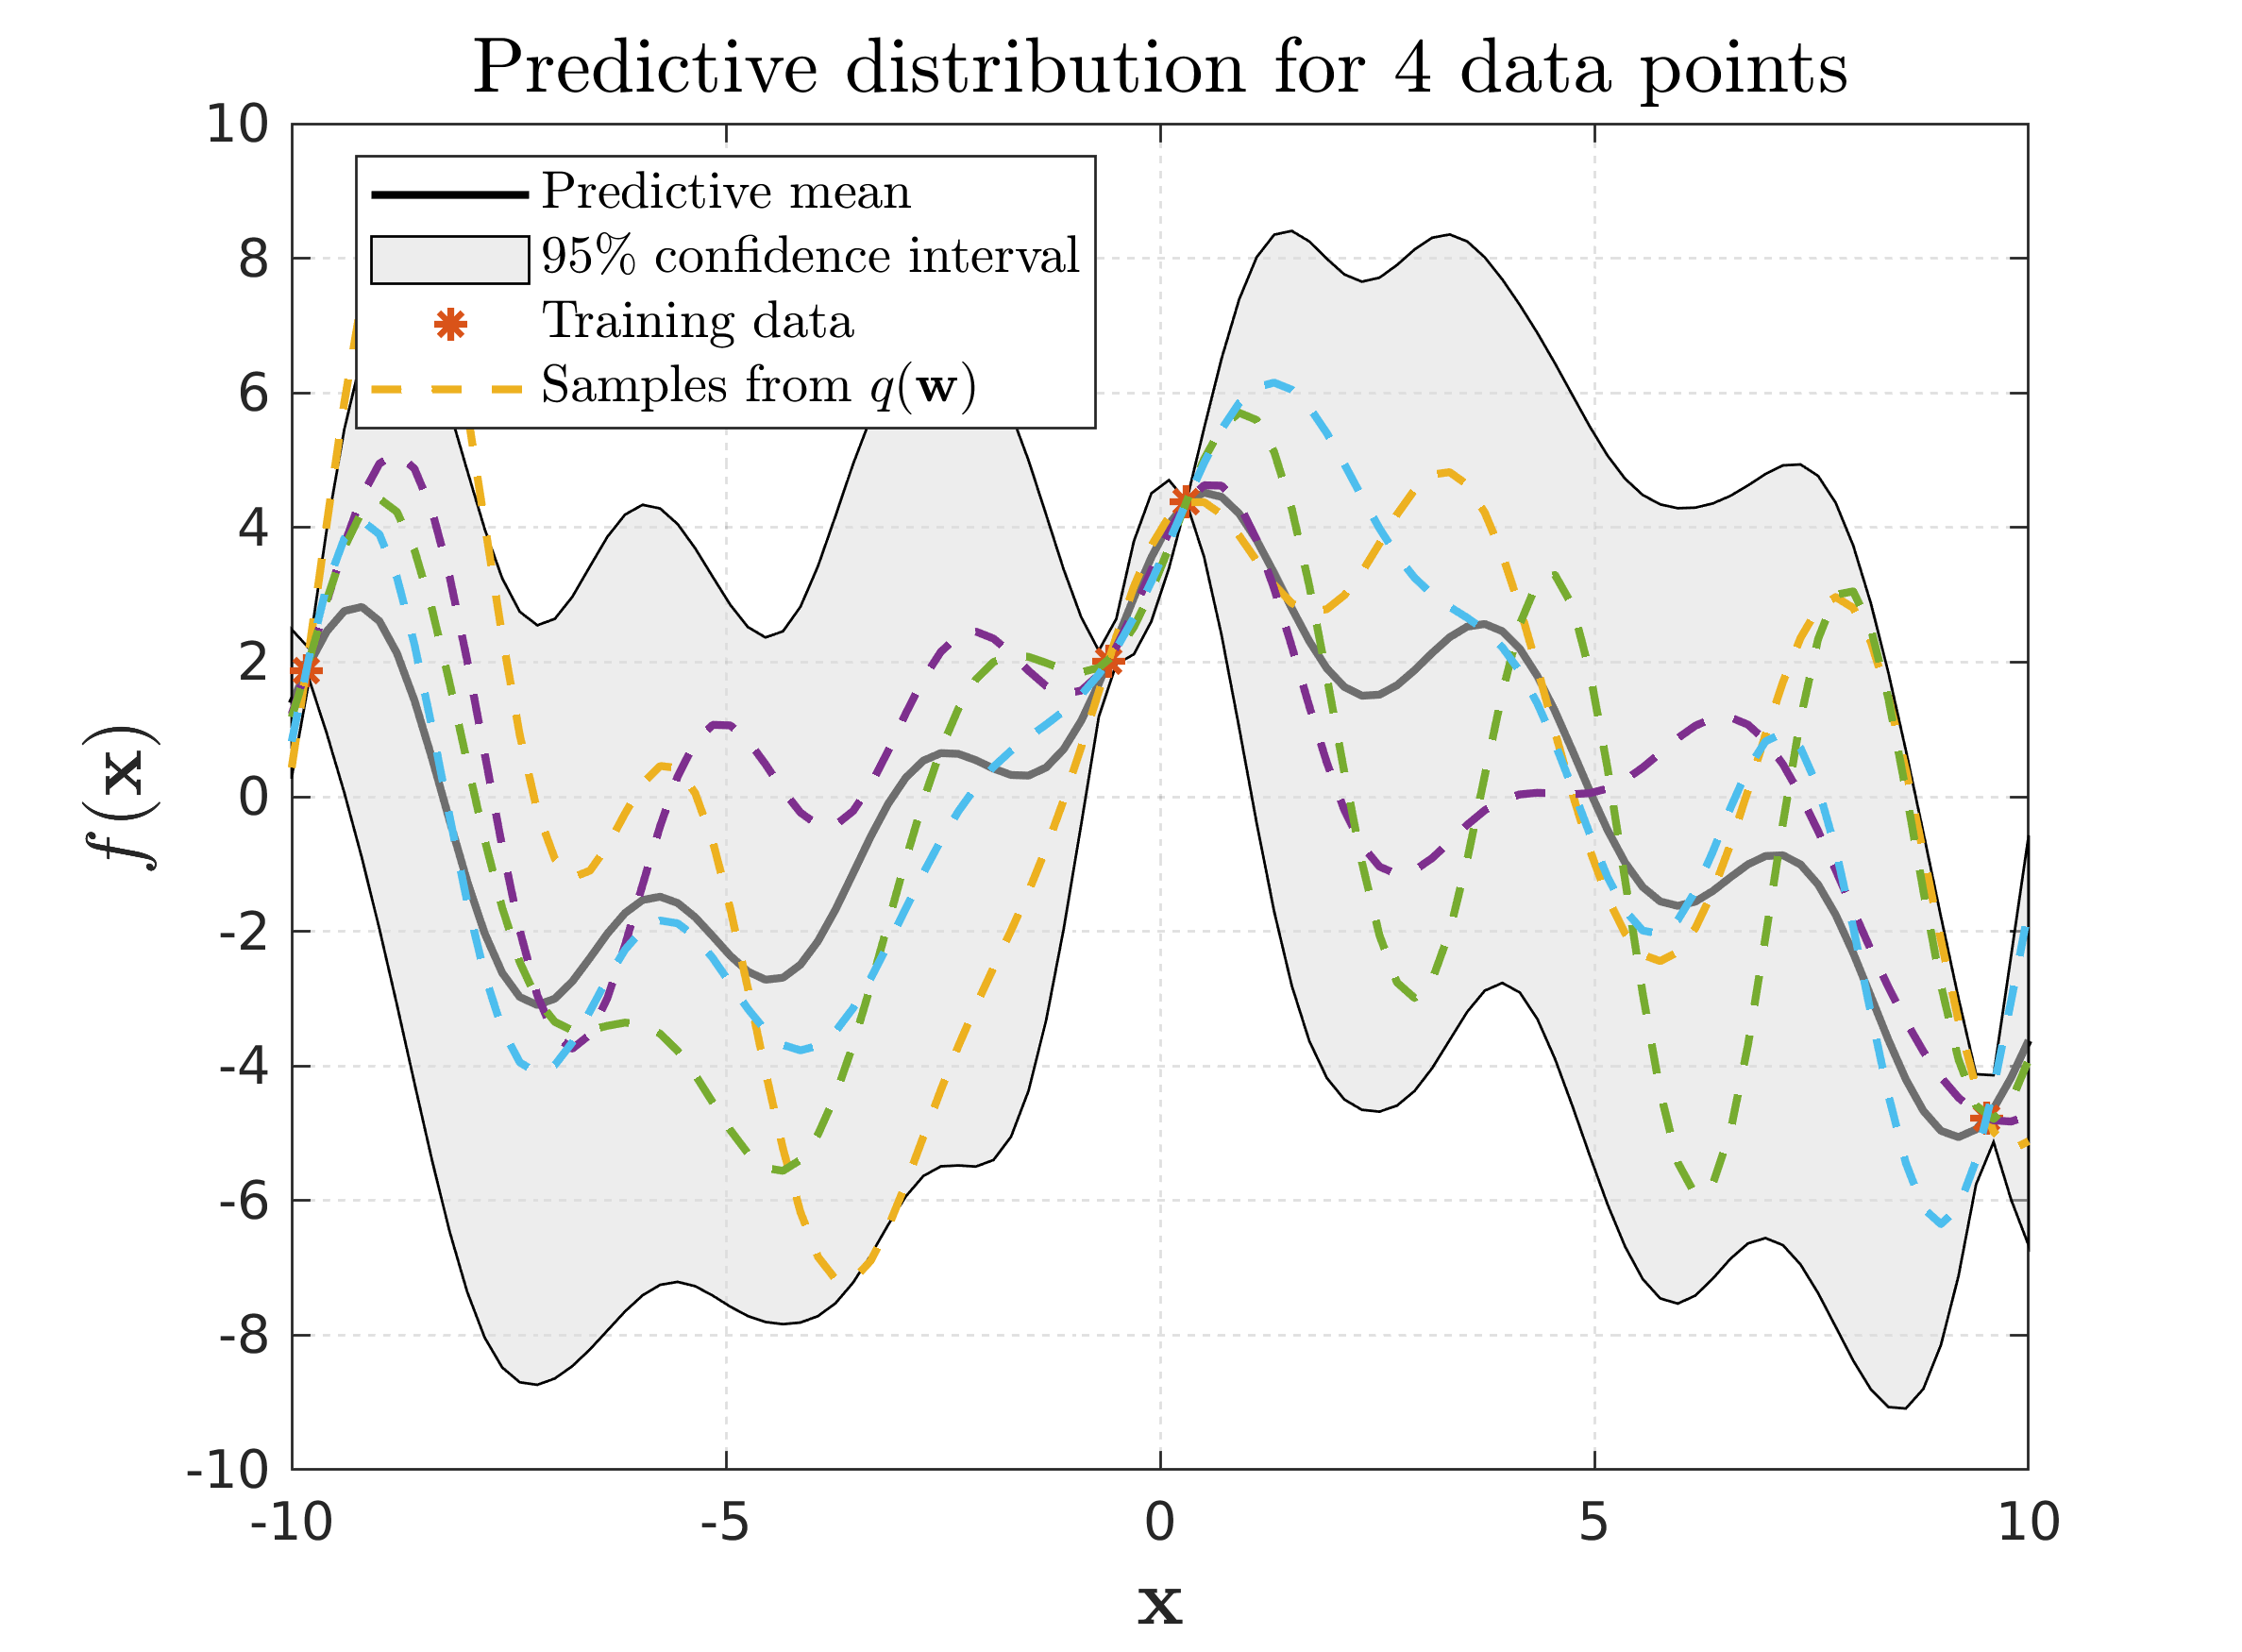
\includegraphics[height=0.4\textheight,width=1\textwidth]{Chapter3/Figures/func_uncertainty_1.png} 
%     \caption{Predictive distribution for 4 data points} 
%     \label{Fig:Re-pred-4-points} 
%   \end{subfigure} 
% %   \hspace{\fill}  %% maximize space between adjacent subfigures
%   \begin{subfigure}[b]{0.49\linewidth}
%     \centering
%     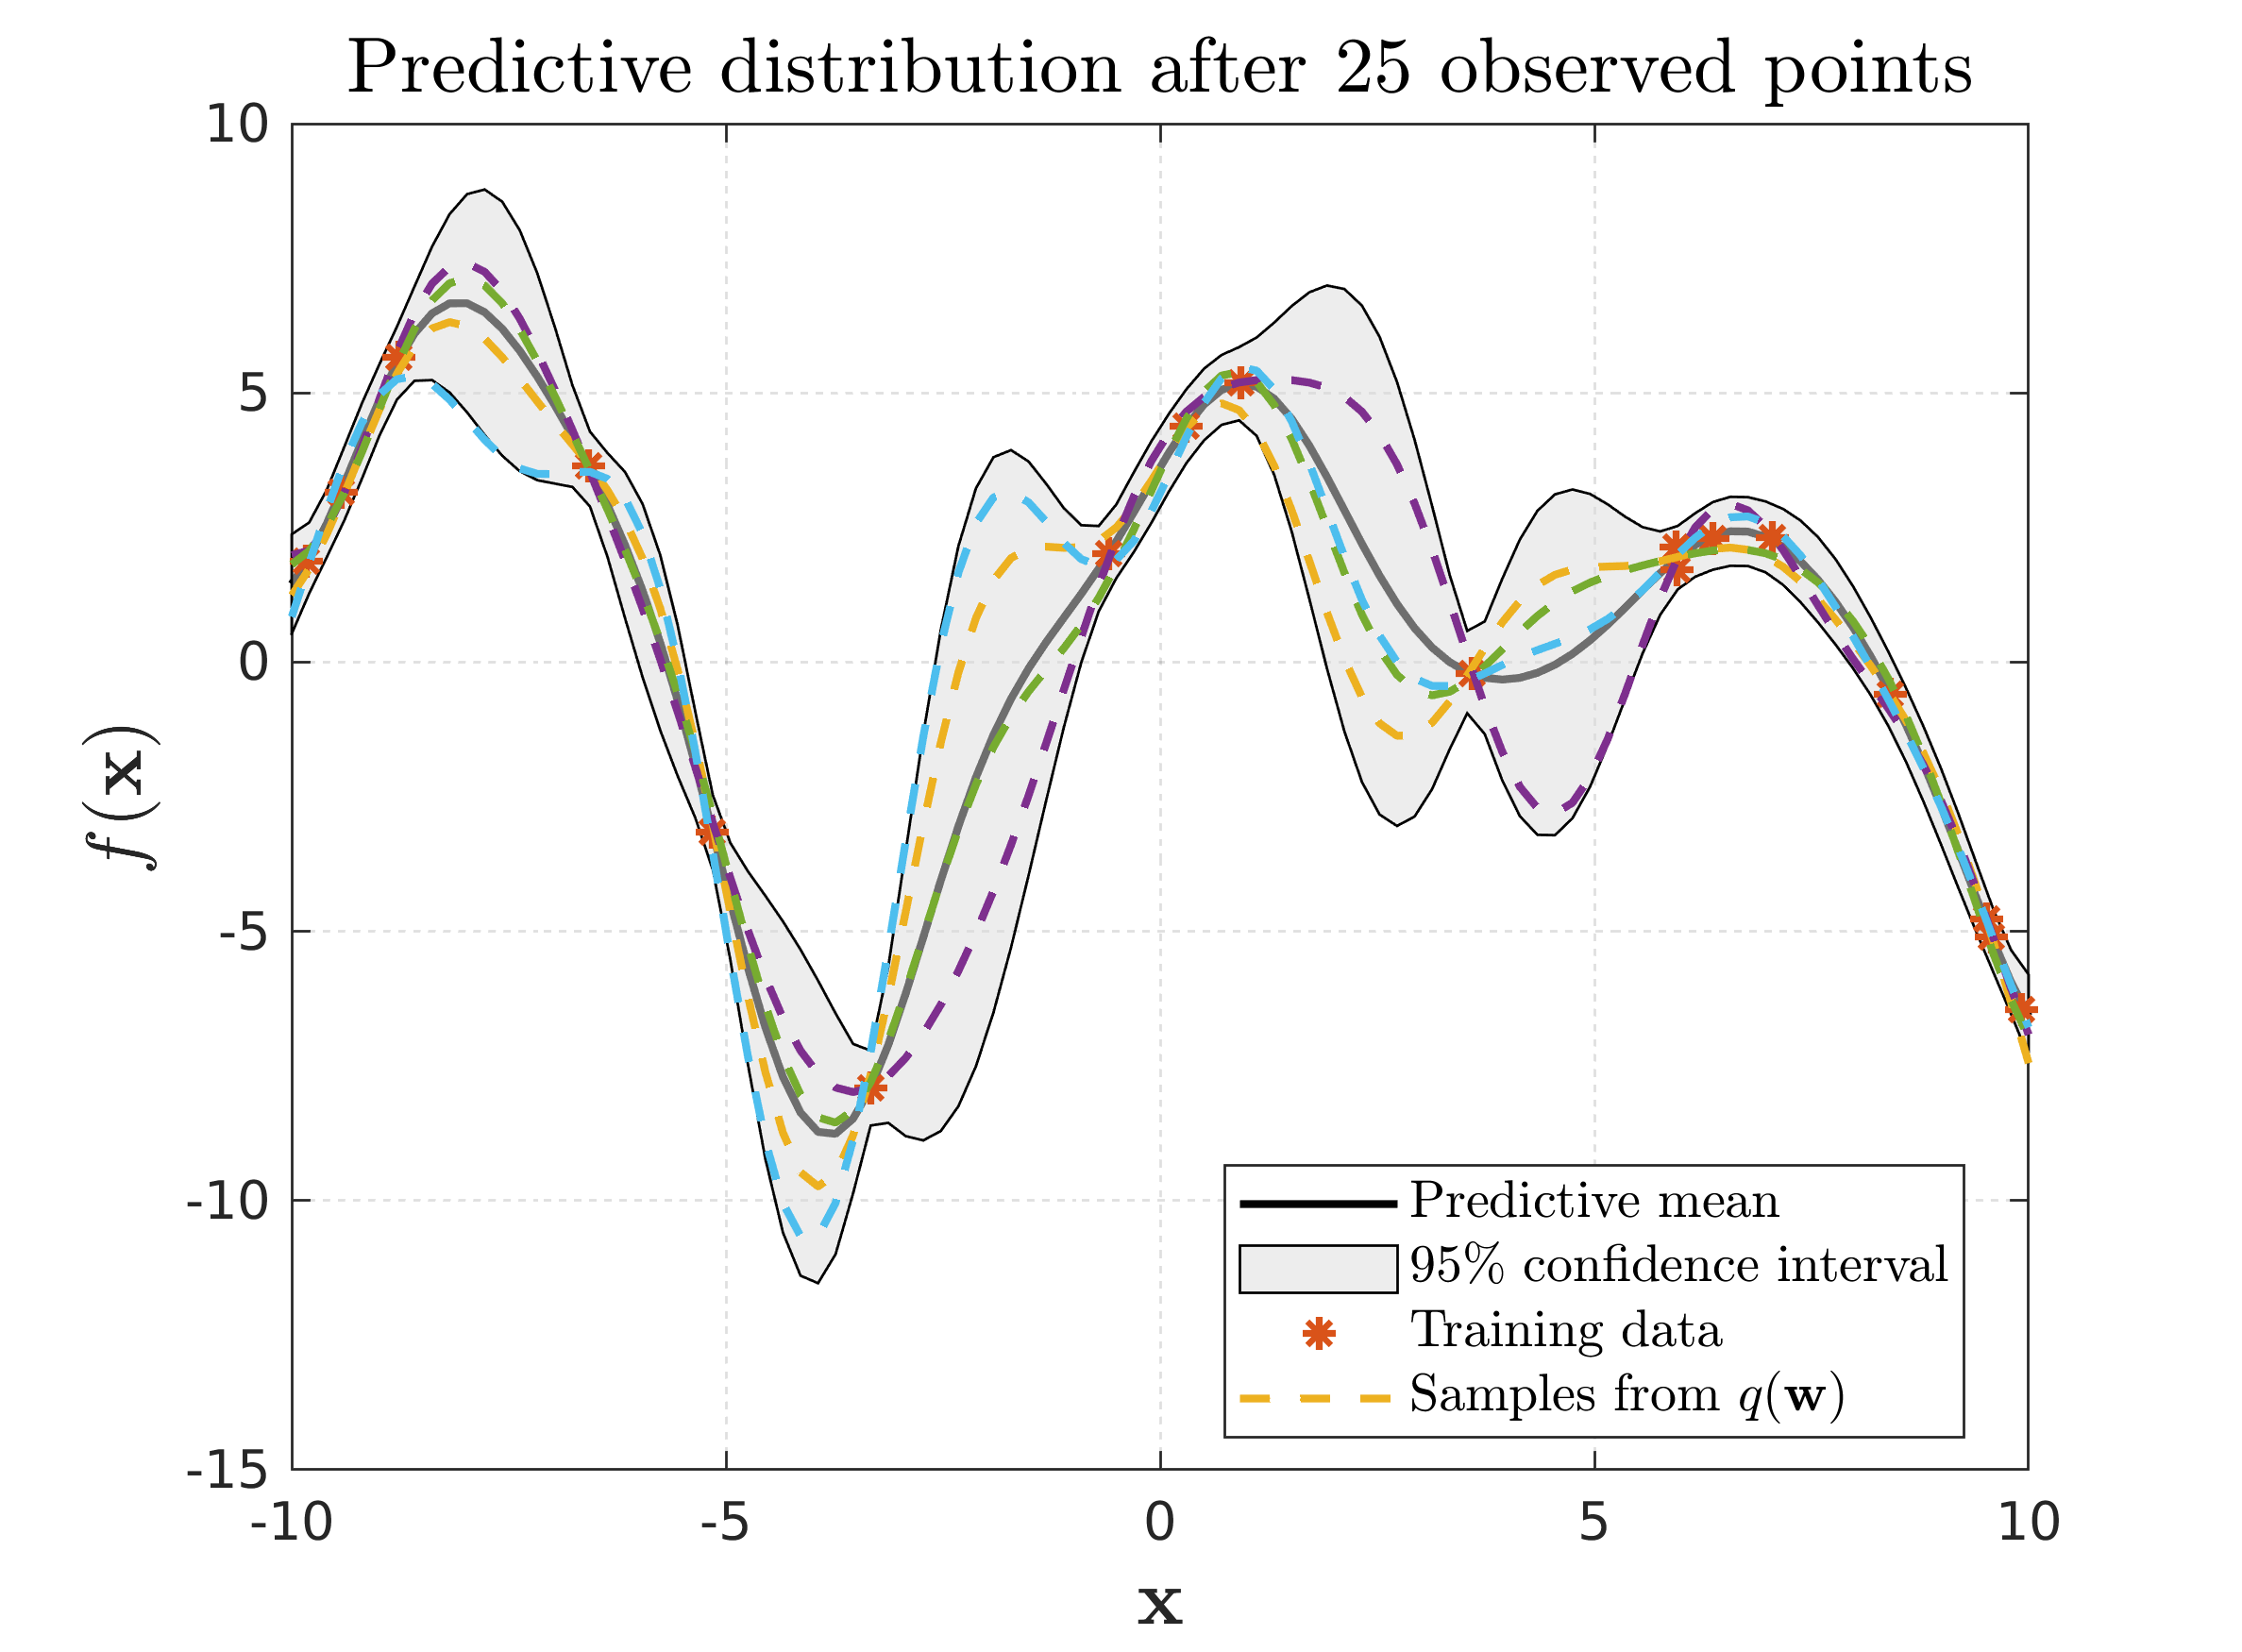
\includegraphics[height=0.4\textheight,width=1\textwidth]{Chapter3/Figures/func_uncertainty_2.png} 
%     \caption{Predictive distribution after 25 data points} 
%     \label{Fig:Re-pred-25-points}
%   \end{subfigure} 

%   \vspace{4ex}  %% extra vertical space
%   \begin{subfigure}[b]{0.49\linewidth}
%     \centering
%     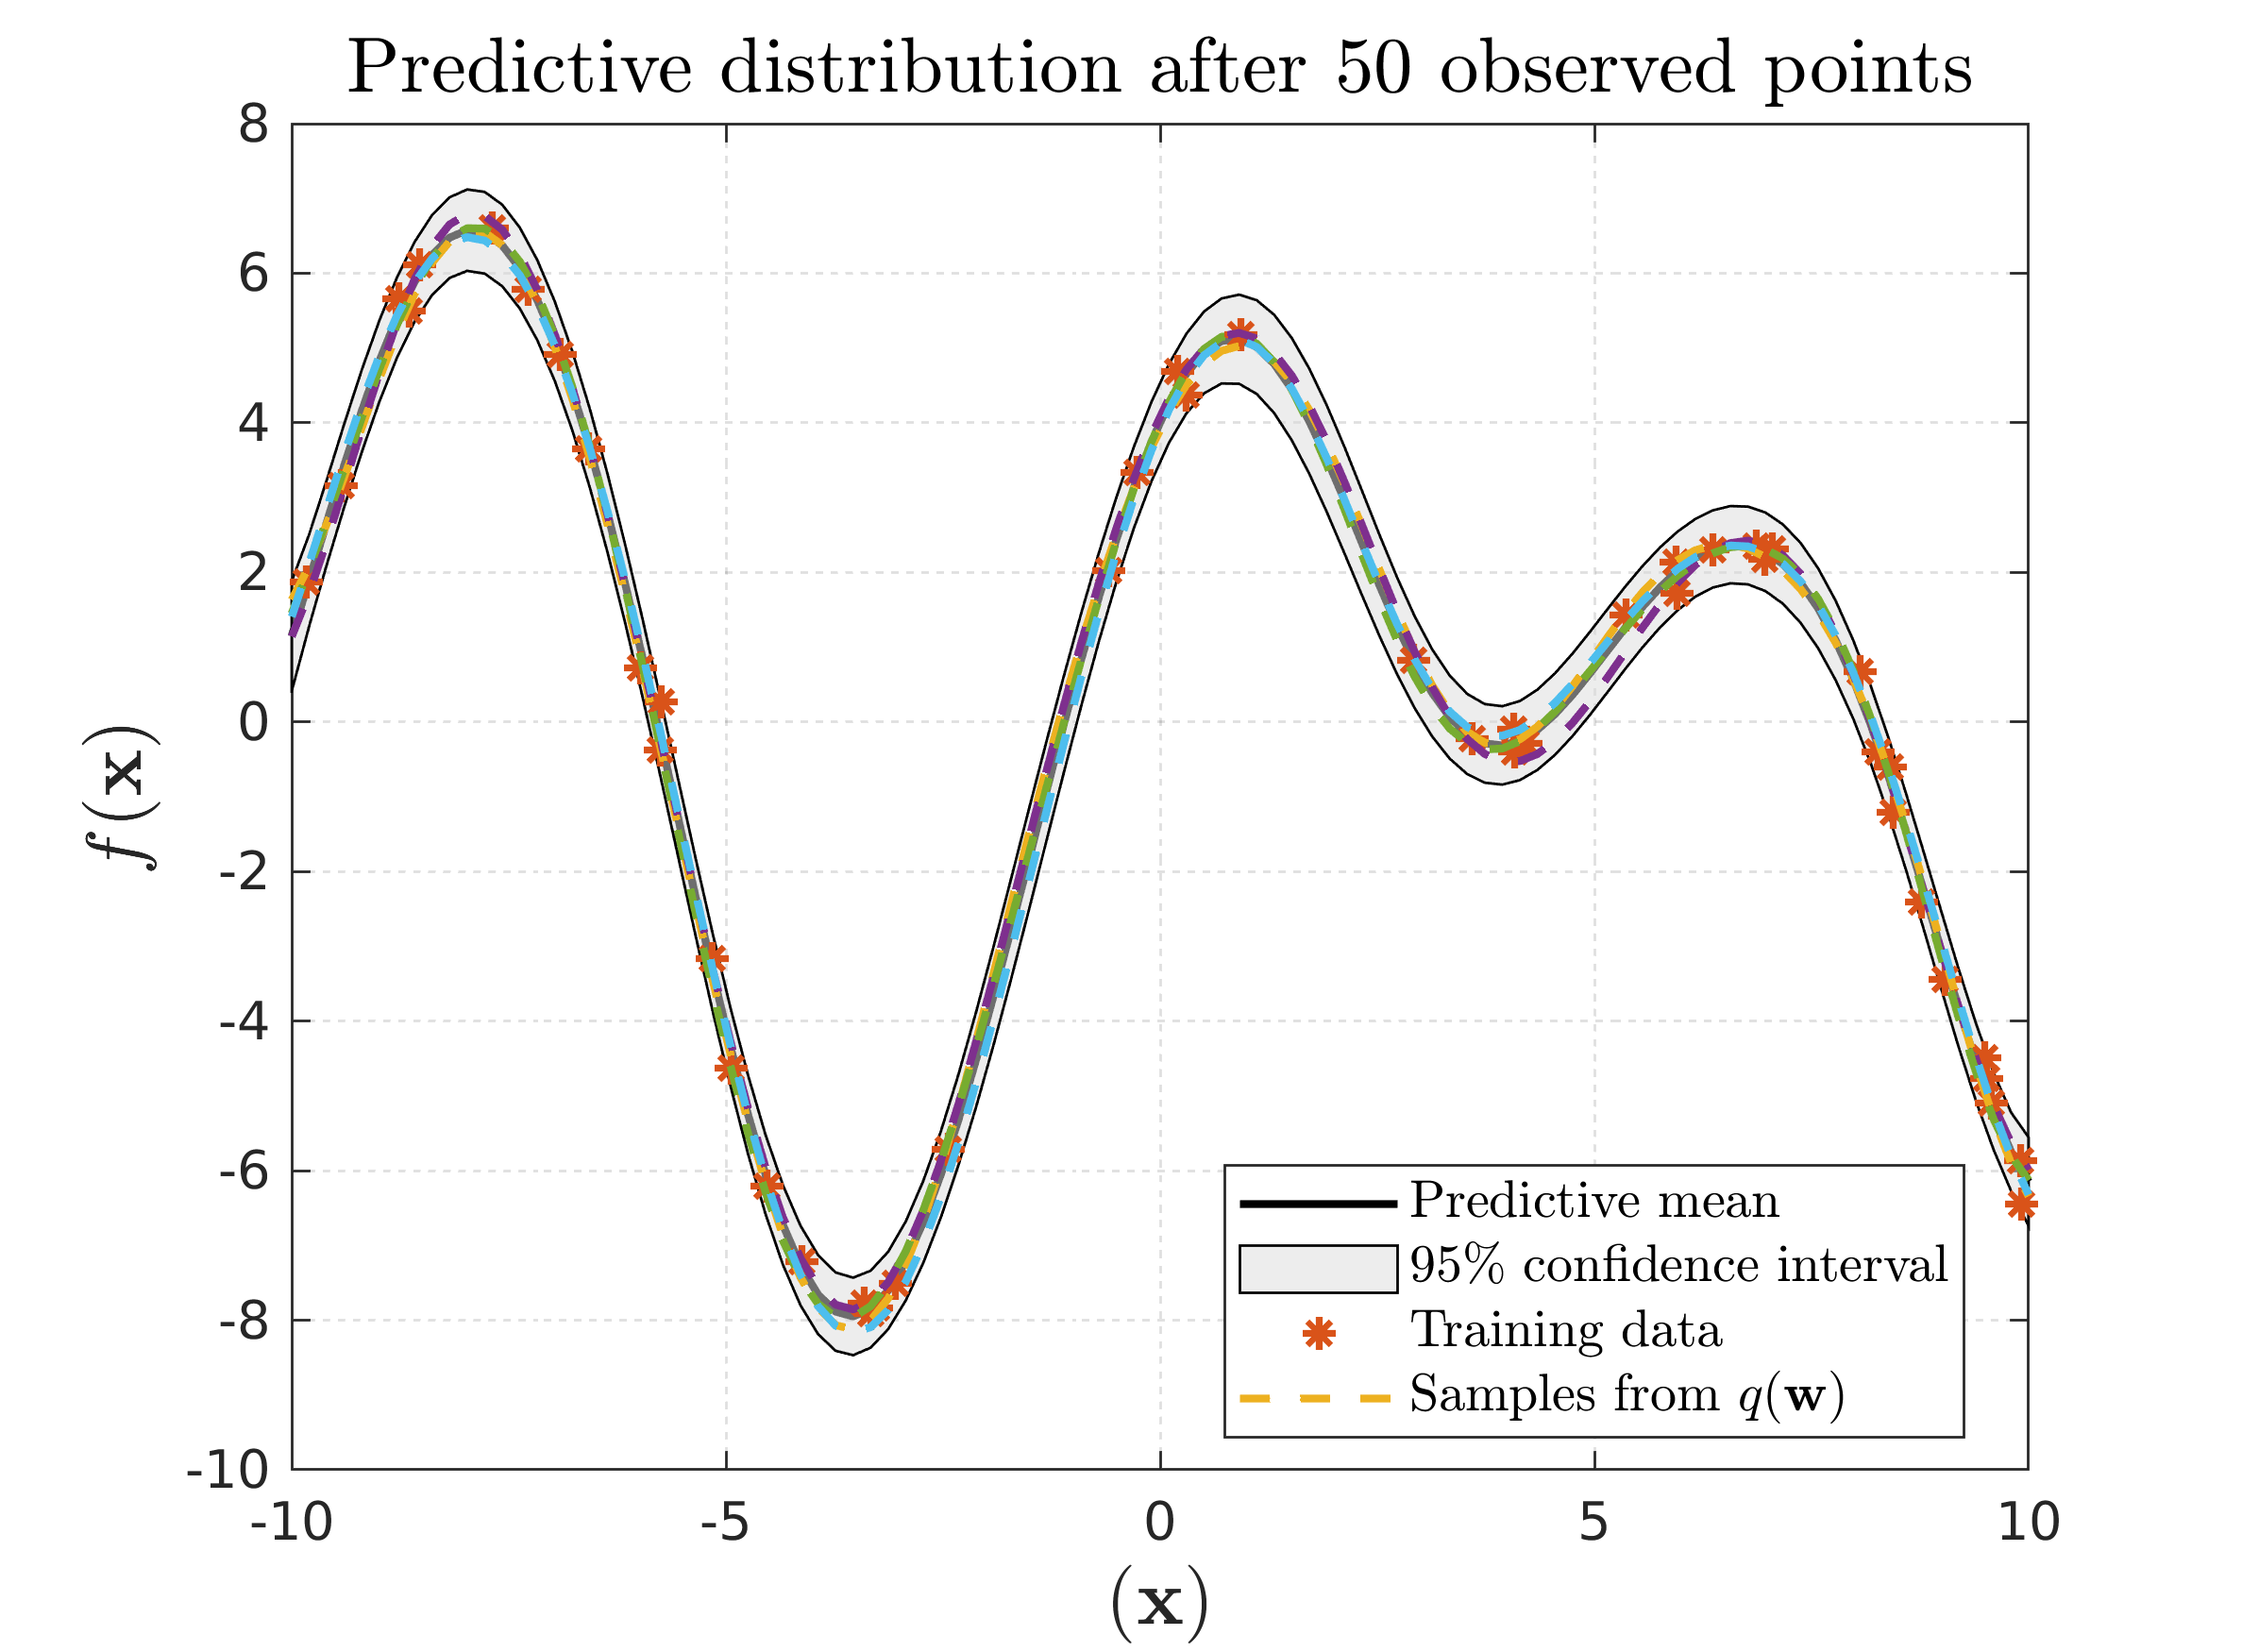
\includegraphics[height=0.4\textheight,width=0.95\textwidth]{Chapter3/Figures/func_uncertainty_3.png} 
%     \caption{Predictive distribution after 50 data points} 
%     \label{Fig:Re-pred-50-points}
%   \end{subfigure} 
% %   \hspace{\fill}
%   \begin{subfigure}[b]{0.49\linewidth}
%     \centering
%     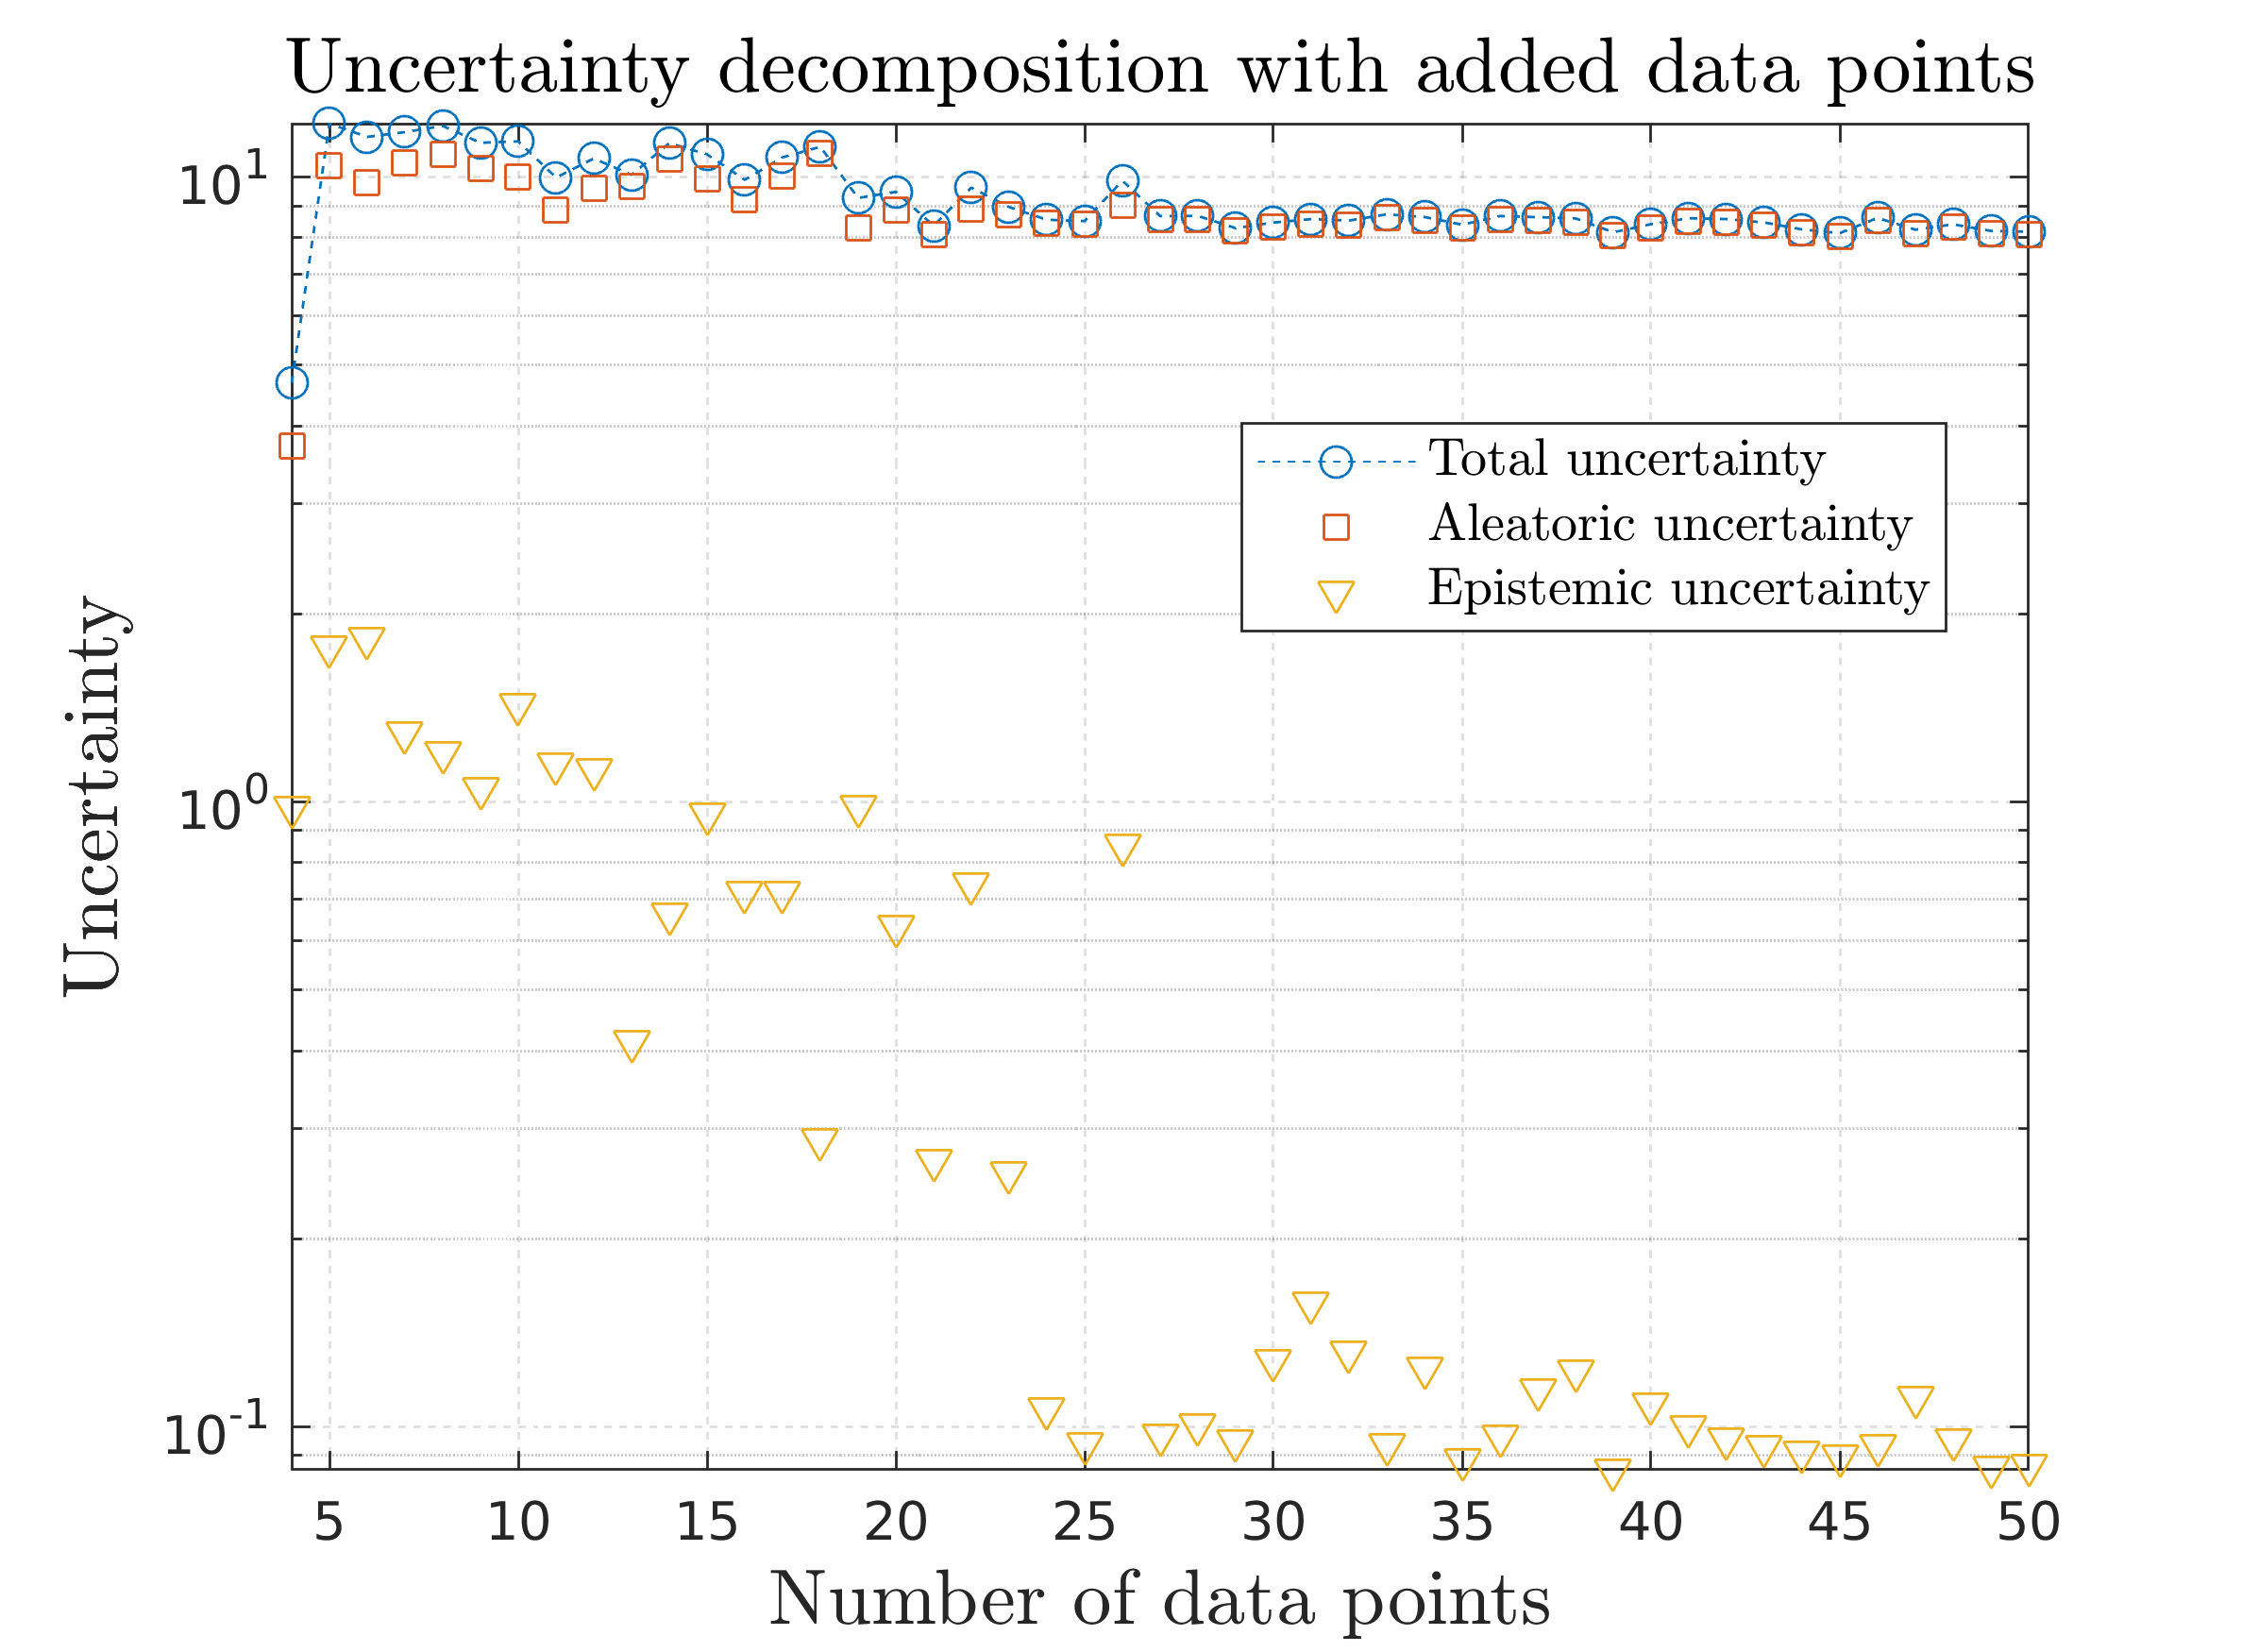
\includegraphics[height=0.4\textheight,width=1\textwidth]{Chapter3/Figures/func_uncertainty_4.png} 
%     \caption{Uncertainty decomposition with added data} 
%     \label{Fig:Re-function-uncertainty} 
%   \end{subfigure} 

% \caption[Reduction in epistemic uncertainty with added data]{: Fig \ref{Fig:Re-pred-4-points} - \ref{Fig:Re-pred-50-points} show the predictive distribution over the data after 4, 25 and 50 data points where the lengthscale of the spectral points purposely set to a high value to over fit the data and imitate high dimensional space. Trajectory rollouts are performed through the transition function for each new data point added and the cost calculated. Fig. \ref{Fig:Re-function-uncertainty} shows that as more data is observed the model becomes increasingly confident about its parameters and consequently the epistemic uncertainty reduces due contraction of the posterior distribution.}
% \label{} 
% \end{figure}
% \end{landscape}

\subsection{Result Cart-Pole}
As the agent interacts with the environment, it exerts its influence through actions which in turn lead a change of state. A carefully crafted set of actions can realise exploration of parts of the state space that are useful in learning the objective.
 In complex problems with large state-spaces only limited parts of the space are relevant to the learning objective and 
\begin{figure}[htp!]    
  \begin{subfigure}[b]{0.48\linewidth}
    \centering
    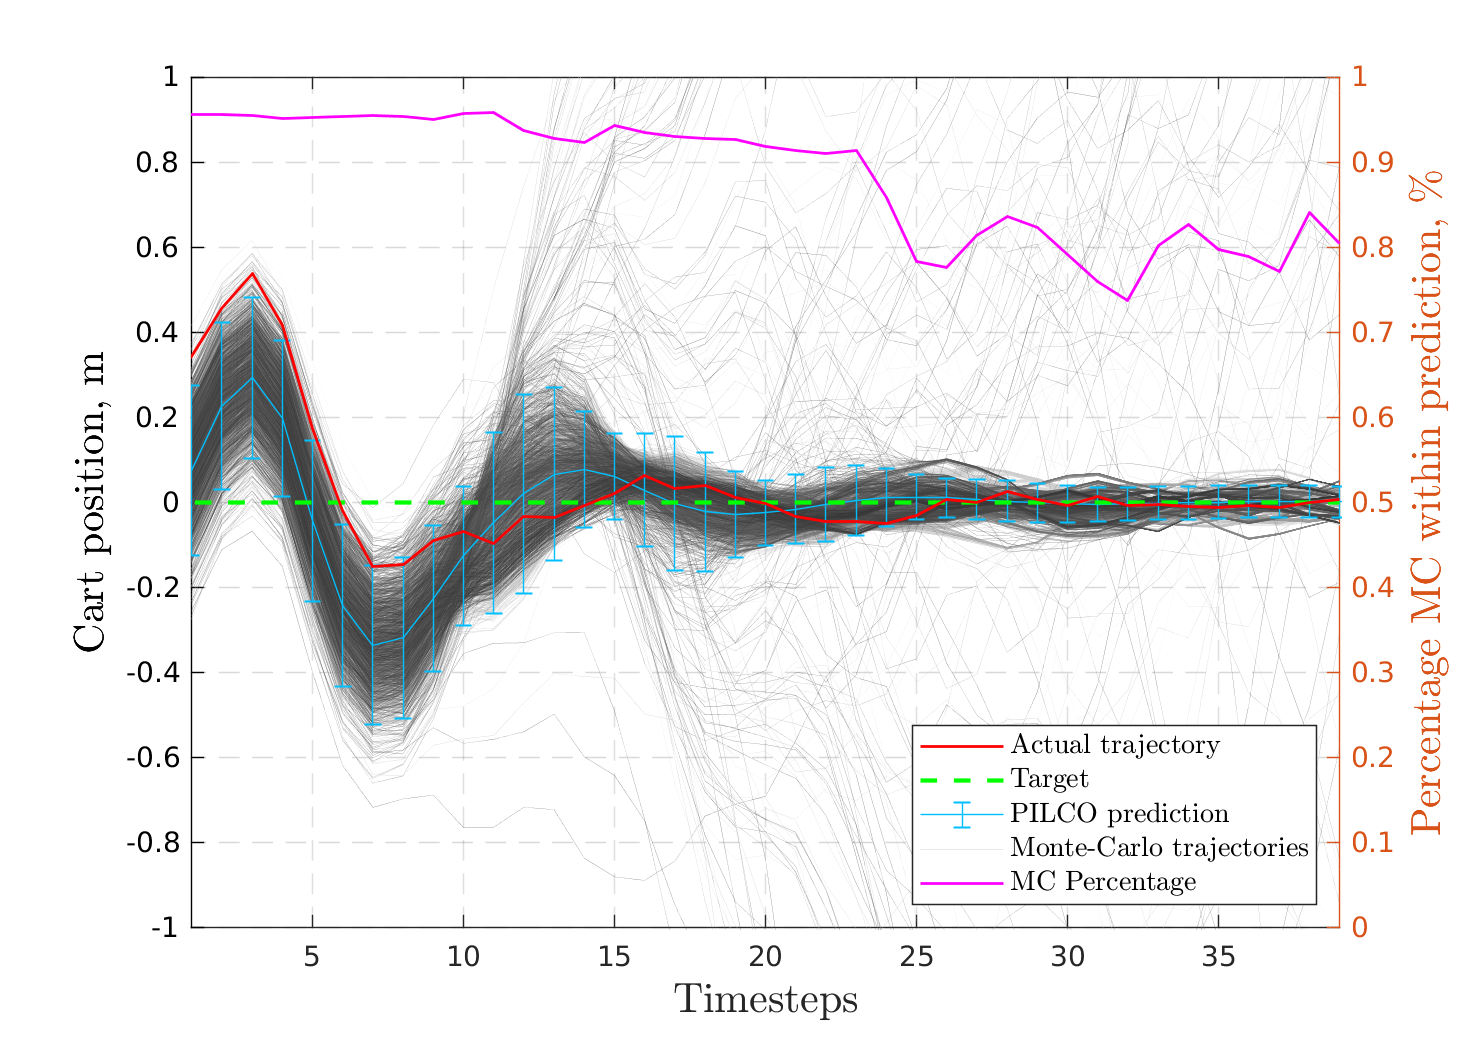
\includegraphics[height=0.22\textheight,width=1\textwidth]{Chapter3/Figures/cp_MC_rollout_Ep_15_Dim_1.png} 
    \caption{Cart position $x$} 
    \label{Fig:Re-cp-cart-position} 
  \end{subfigure} 
  \hspace{\fill}  %% maximize space between adjacent subfigures
  \begin{subfigure}[b]{0.48\linewidth}
    \centering
    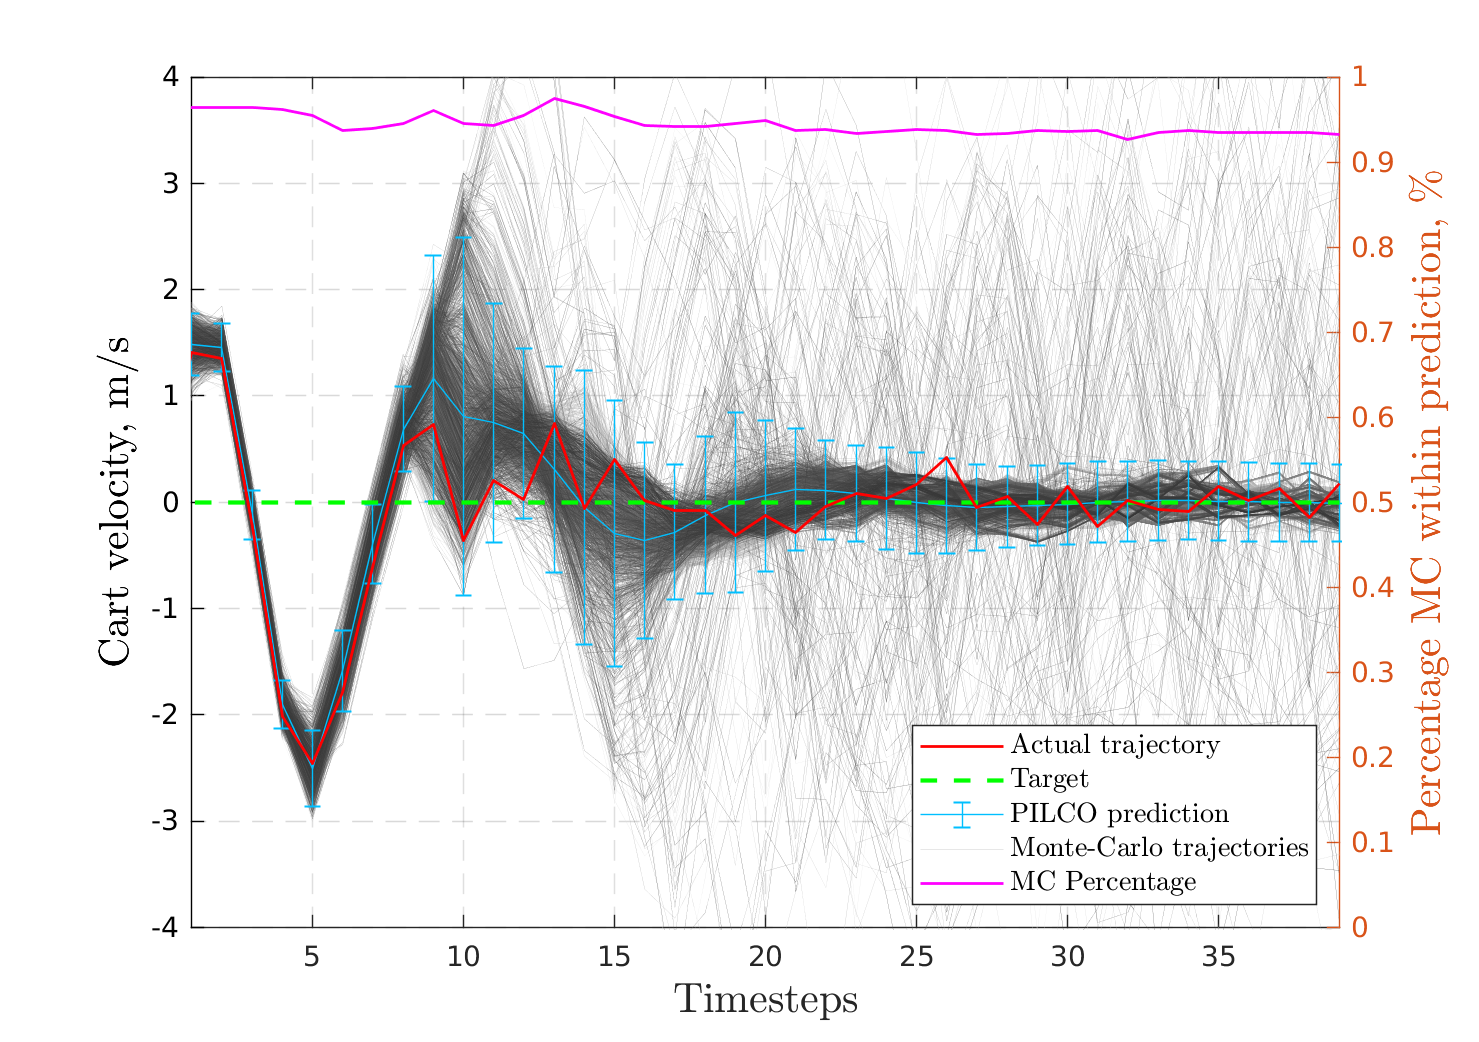
\includegraphics[height=0.22\textheight,width=1\textwidth]{Chapter3/Figures/cp_MC_rollout_Ep_15_Dim_2.png} 
    \caption{Cart velocity $\dot x$} 
    \label{Fig:Re-cp-cart-velocity} 
  \end{subfigure} 

  \vspace{4ex}  %% extra vertical space
  \begin{subfigure}[b]{0.48\linewidth}
    \centering
    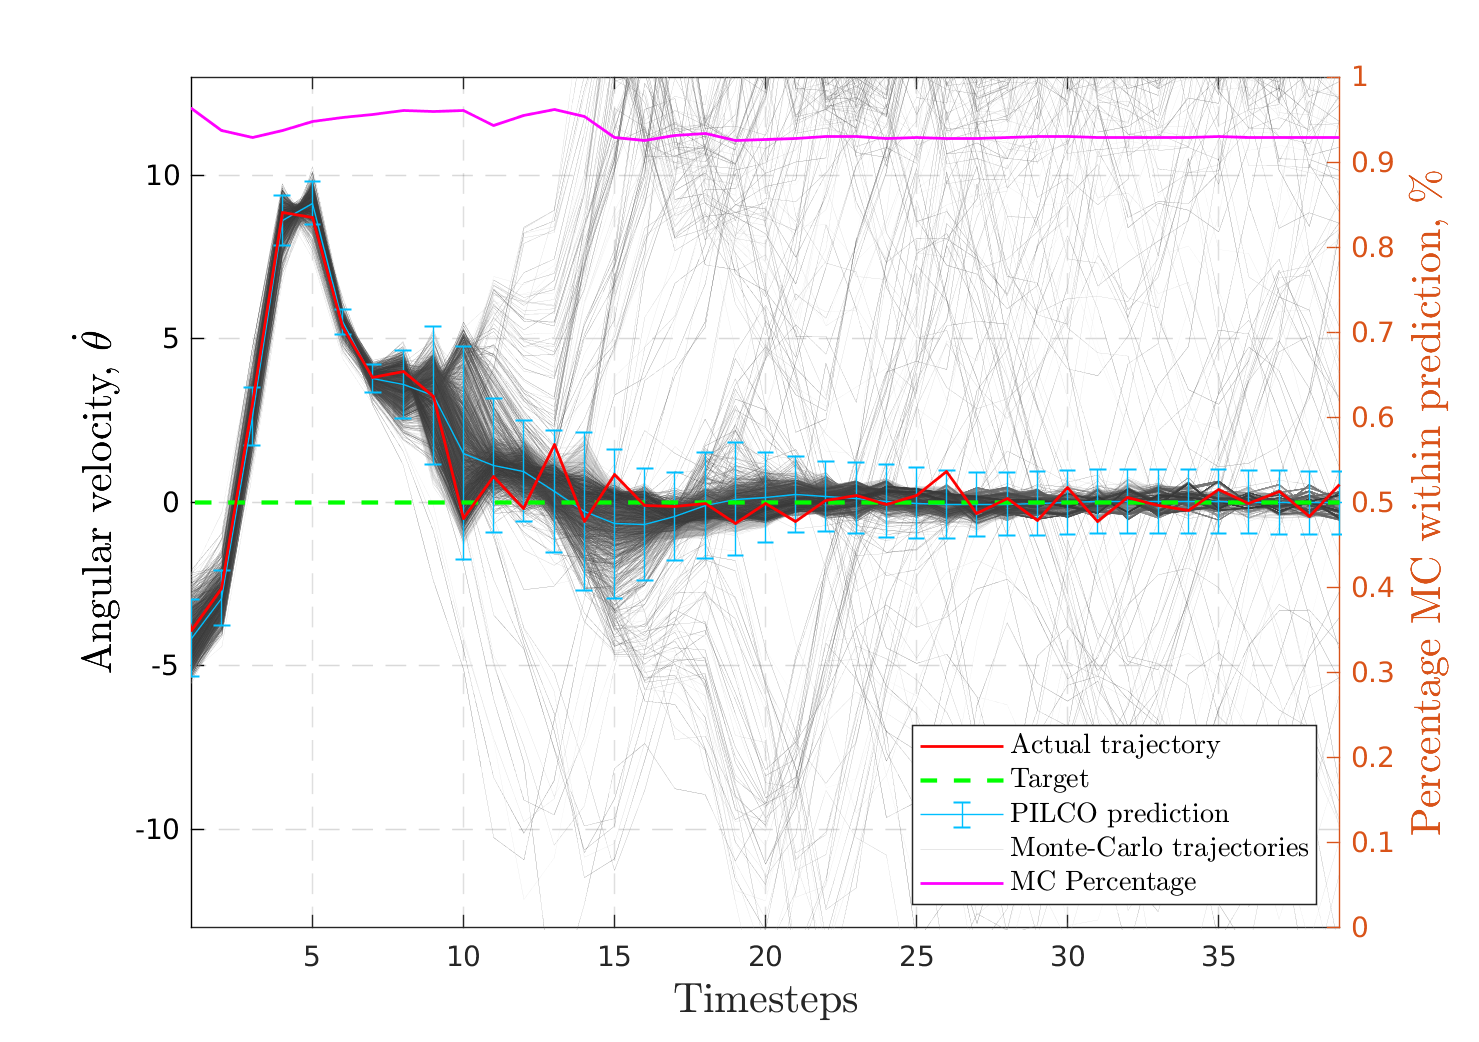
\includegraphics[height=0.22\textheight,width=1\textwidth]{Chapter3/Figures/cp_MC_rollout_Ep_15_Dim_3.png} 
    \caption{Pendulum angular velocity $\dot \theta$} 
    \label{Fig:Re-cp-pen-velocity} 
  \end{subfigure} 
  \hspace{\fill}
  \begin{subfigure}[b]{0.48\linewidth}
    \centering
    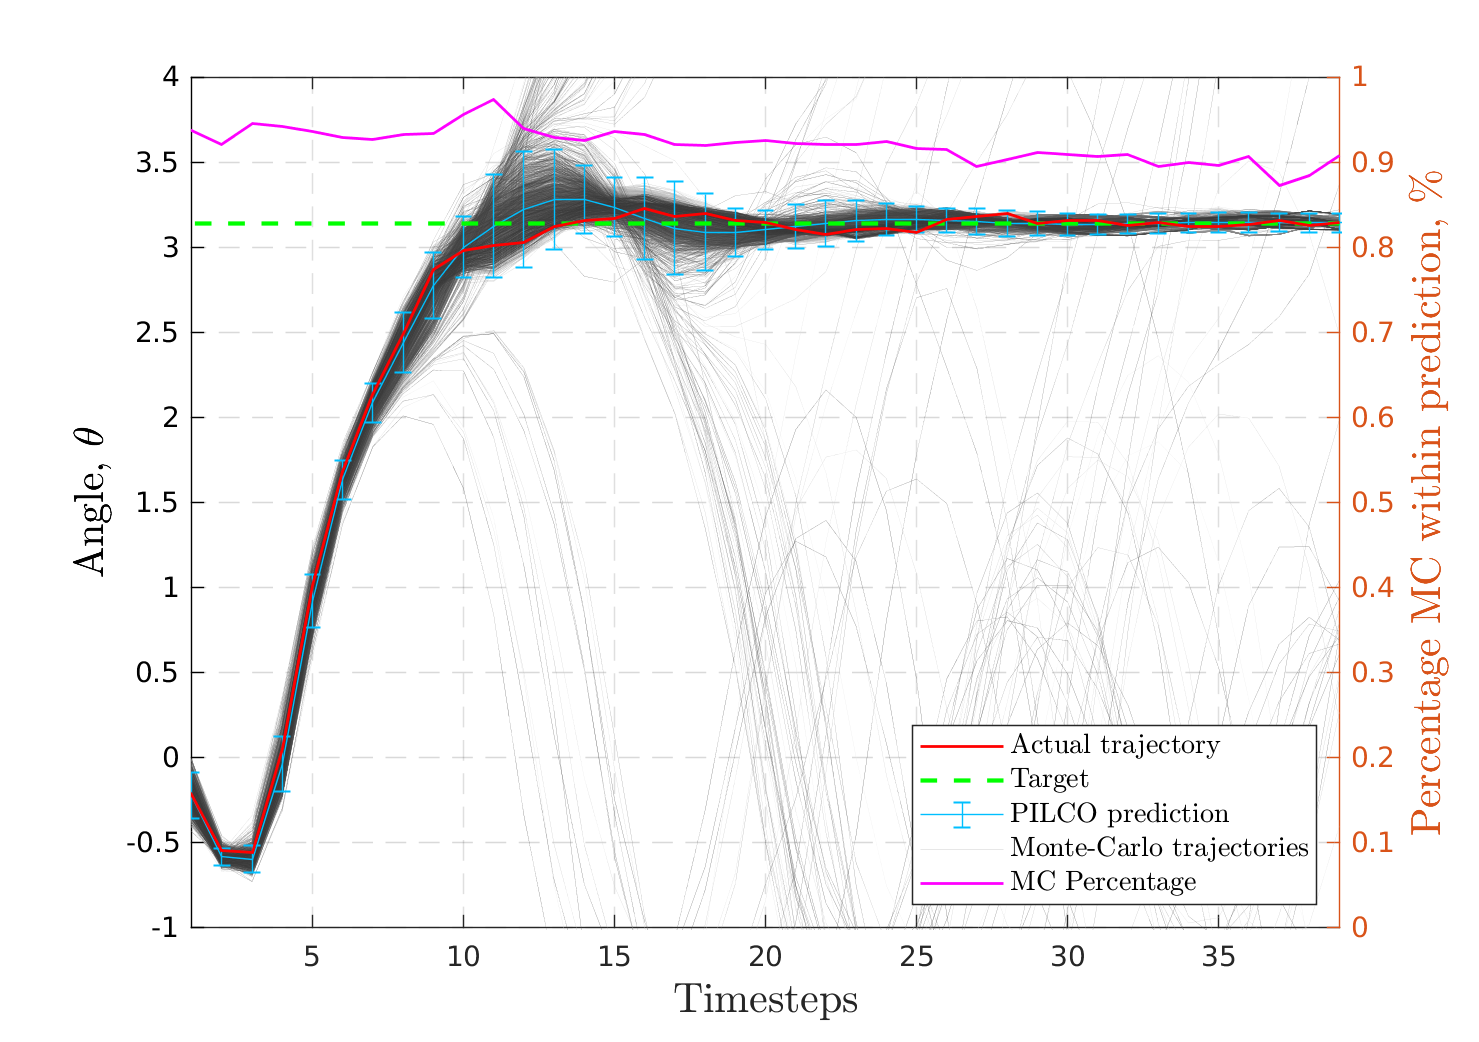
\includegraphics[height=0.22\textheight,width=1\textwidth]{Chapter3/Figures/cp_MC_rollout_Ep_15_Dim_4.png} 
    \caption{Pendulum angle $\theta$} 
    \label{Fig:Re-cp-pen-angle} 
  \end{subfigure} 

    \vspace{4ex}
  \begin{subfigure}[b]{0.48\linewidth}
    \centering
    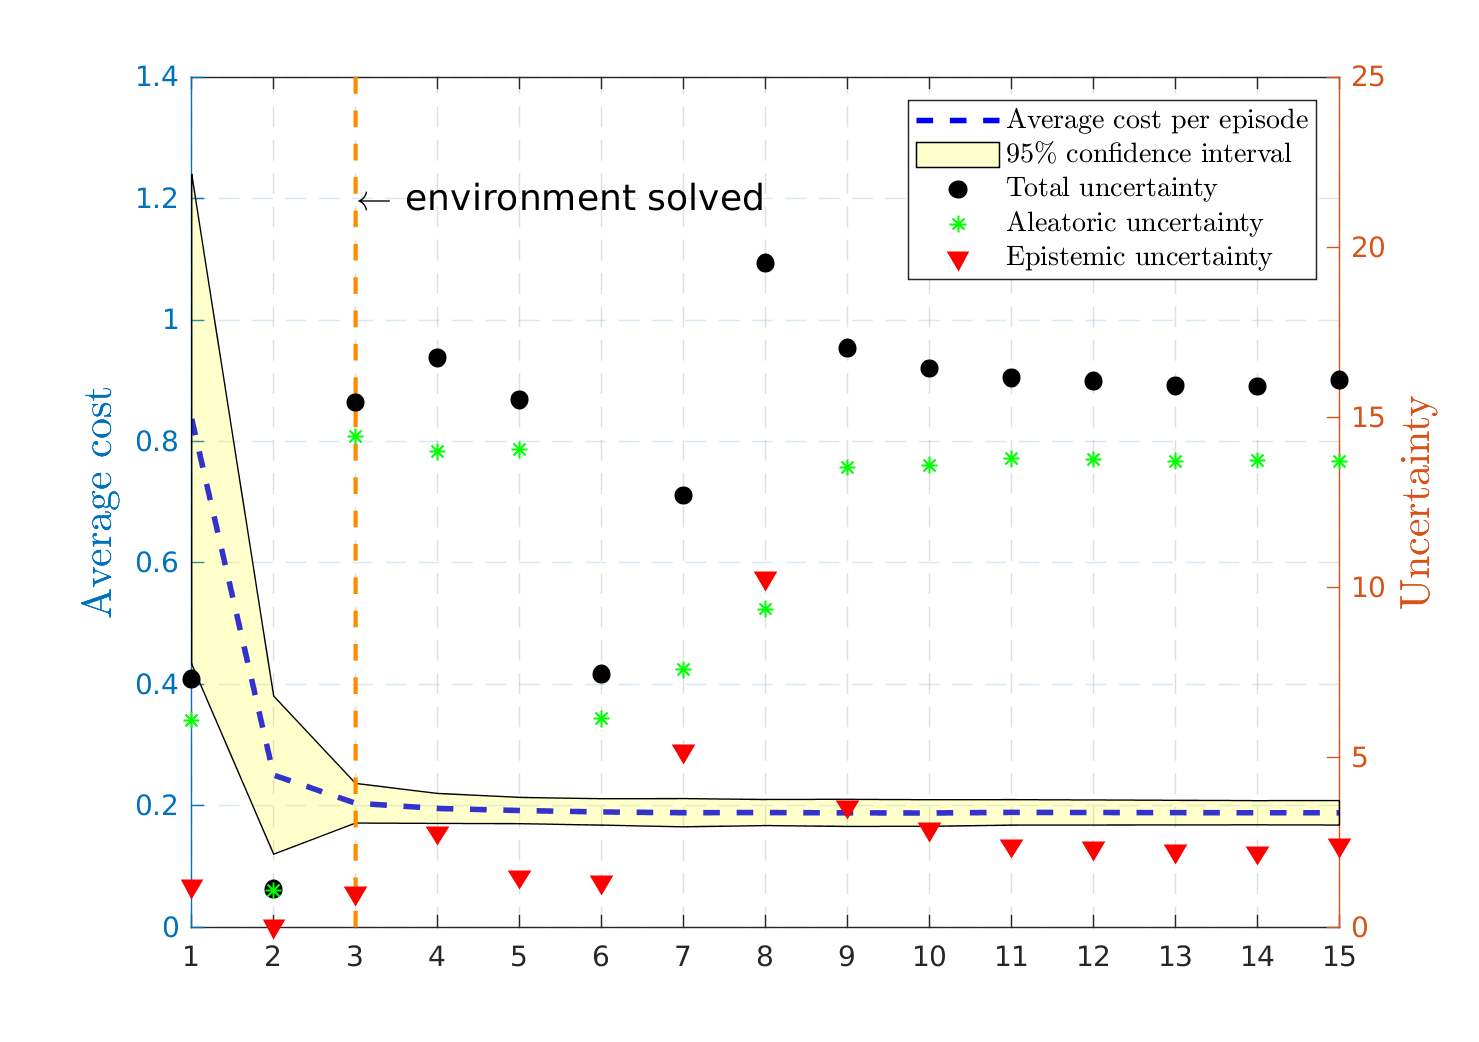
\includegraphics[height=0.22\textheight,width=1\textwidth]{Chapter3/Figures/cp_uncertainty.png} 
    \caption{Average cost (left axis) and uncertainty decomposition (right axis) for each episode over the course of learning.} 
    \label{Fig:Re-cp-uncertainty} 
  \end{subfigure}
  \hspace{\fill}
  \begin{subfigure}[b]{0.48\linewidth}
    \centering
    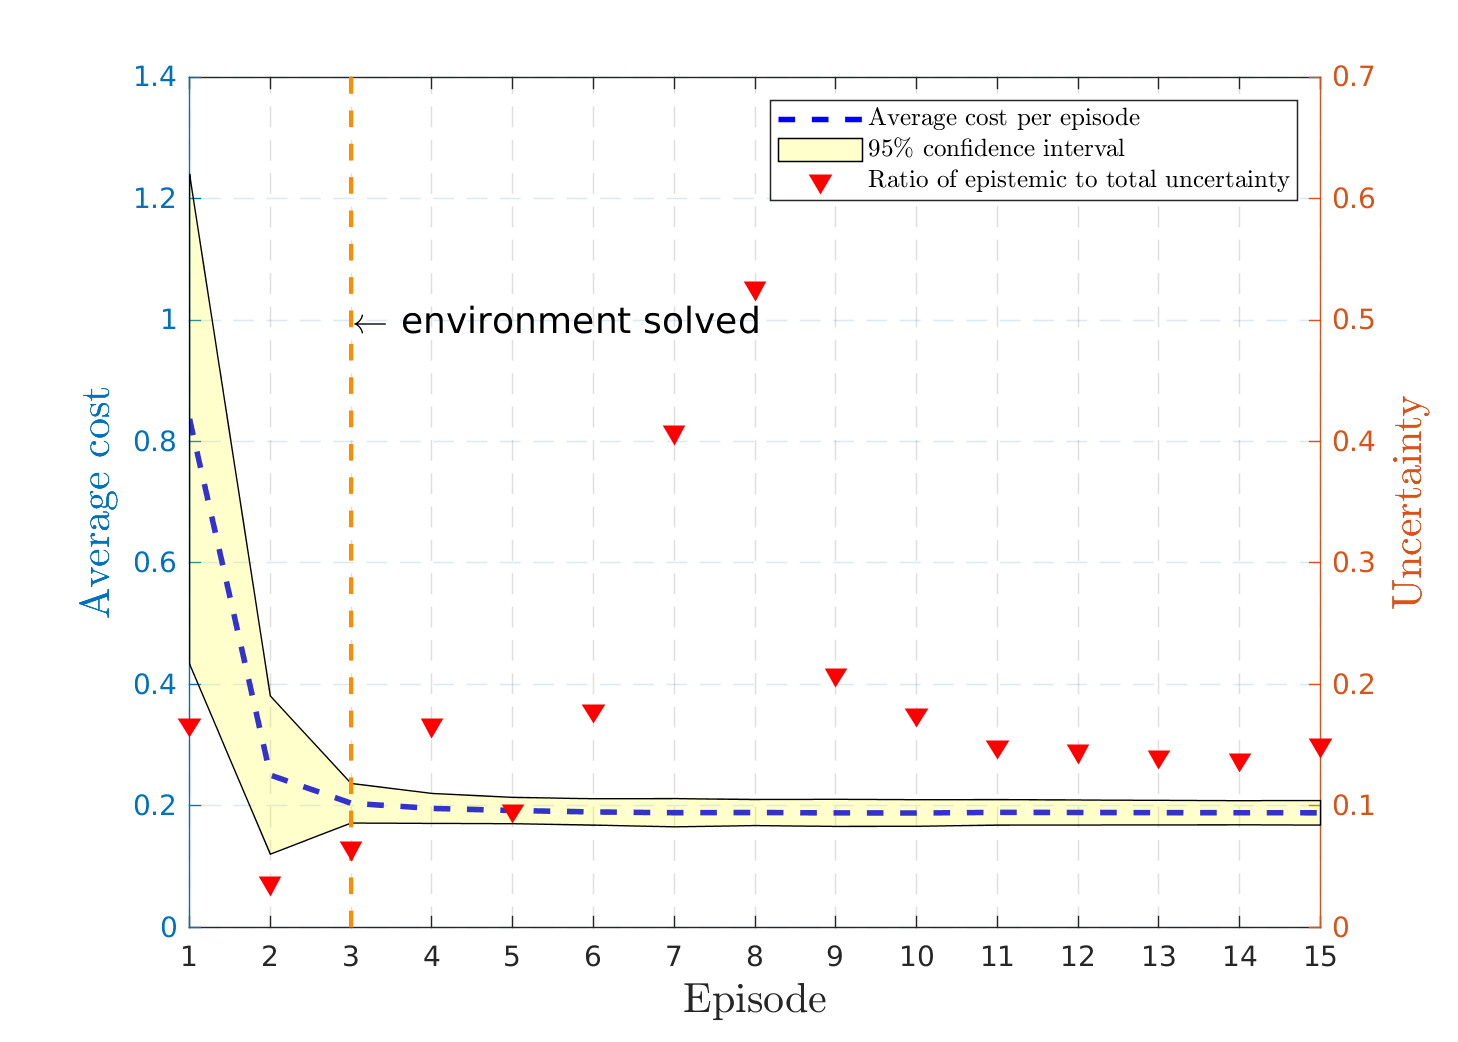
\includegraphics[height=0.22\textheight,width=1\textwidth]{Chapter3/Figures/cp_uncertainty_norm.png} 
    \caption{Average cost (left axis) and ratio of epistemic to total uncertainty (right axis) for each episode over the course of learning.} 
    \label{Fig:Re-cp-uncertainty-norm} 
  \end{subfigure} 
\caption[Monte-Carlo uncertainty decomposition for for \textbf{cart-pole} environment]{Monte-Carlo uncertainty decomposition for the \textbf{cart-pole} environment. Figs. \ref{Fig:Re-cp-cart-position} - \ref{Fig:Re-cp-pen-angle} show a random sample of the Monte-Carlo trajectories for each of the state variables for episode 15. The first three legend items (actual trajectory, target, PILCO prediction and MC trajectories) correspond to the state variable axis (left axis) and the magenta line shows the percentage of MC trajectories inside PILCO's prediction (2 standard deviations) (right axis).  Figs. \ref{Fig:Re-cp-uncertainty} - \ref{Fig:Re-cp-uncertainty-norm} show the average cost (left axis) and uncertainty (right axis) for each episode over the course of learning.}
\label{Fig:Re-Cart-Pole-Full-Results} 
\end{figure}

\subsection{Results Pendubot}

\begin{figure}[htp!]    
  \begin{subfigure}[b]{0.48\linewidth}
    \centering
    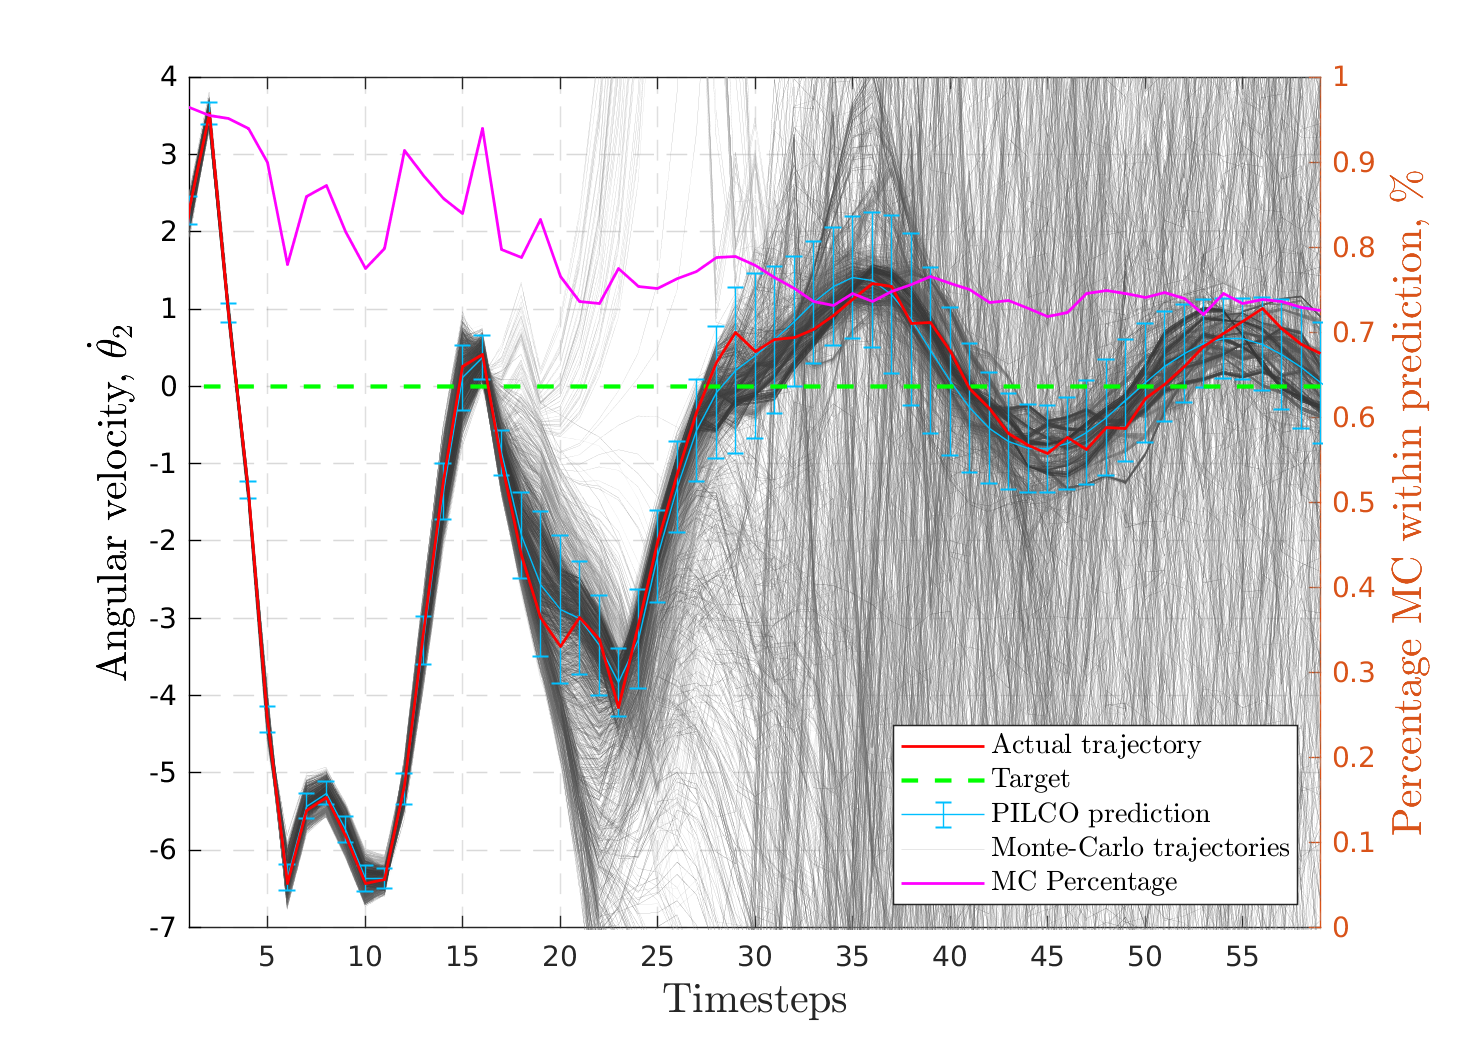
\includegraphics[height=0.22\textheight,width=1\textwidth]{Chapter3/Figures/pen_MC_rollout_Ep_40_Dim_1.png} 
    \caption{Pendulum angular velocity $\dot \theta_{2}$} 
    \label{Fig:Re-pen-cart-position} 
  \end{subfigure} 
  \hspace{\fill}  %% maximize space between adjacent subfigures
  \begin{subfigure}[b]{0.48\linewidth}
    \centering
    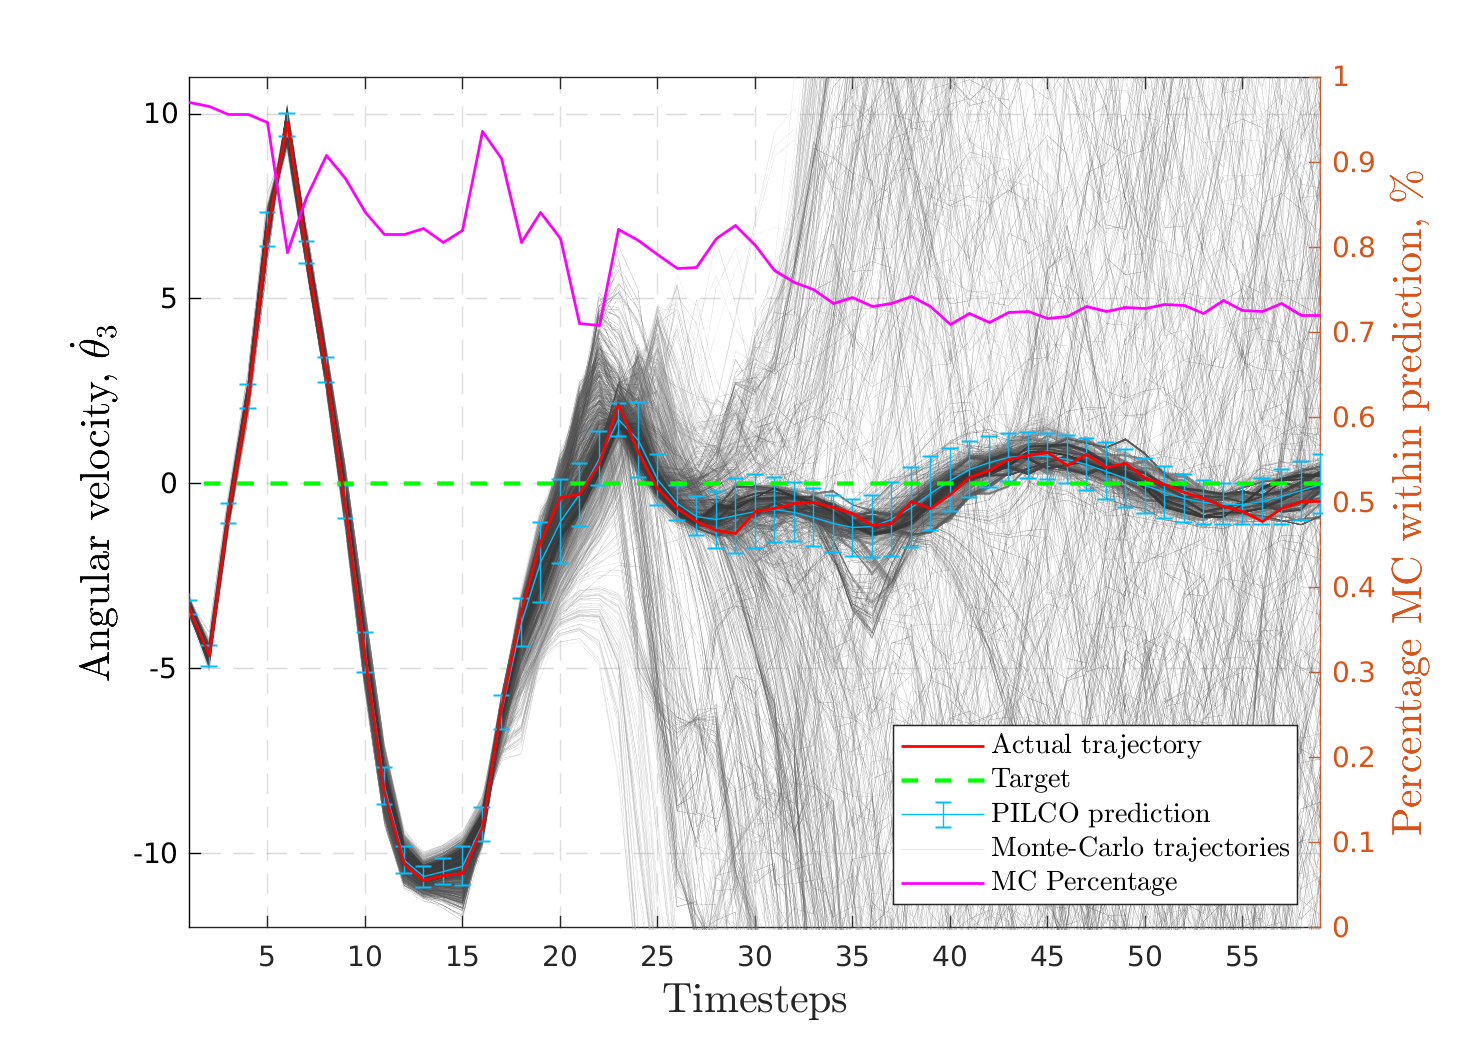
\includegraphics[height=0.22\textheight,width=1\textwidth]{Chapter3/Figures/pen_MC_rollout_Ep_40_Dim_2.png} 
    \caption{Pendulum angular velocity $\dot \theta_{3}$} 
    \label{Fig:Re-pen-cart-velocity} 
  \end{subfigure} 

  \vspace{4ex}  %% extra vertical space
  \begin{subfigure}[b]{0.48\linewidth}
    \centering
    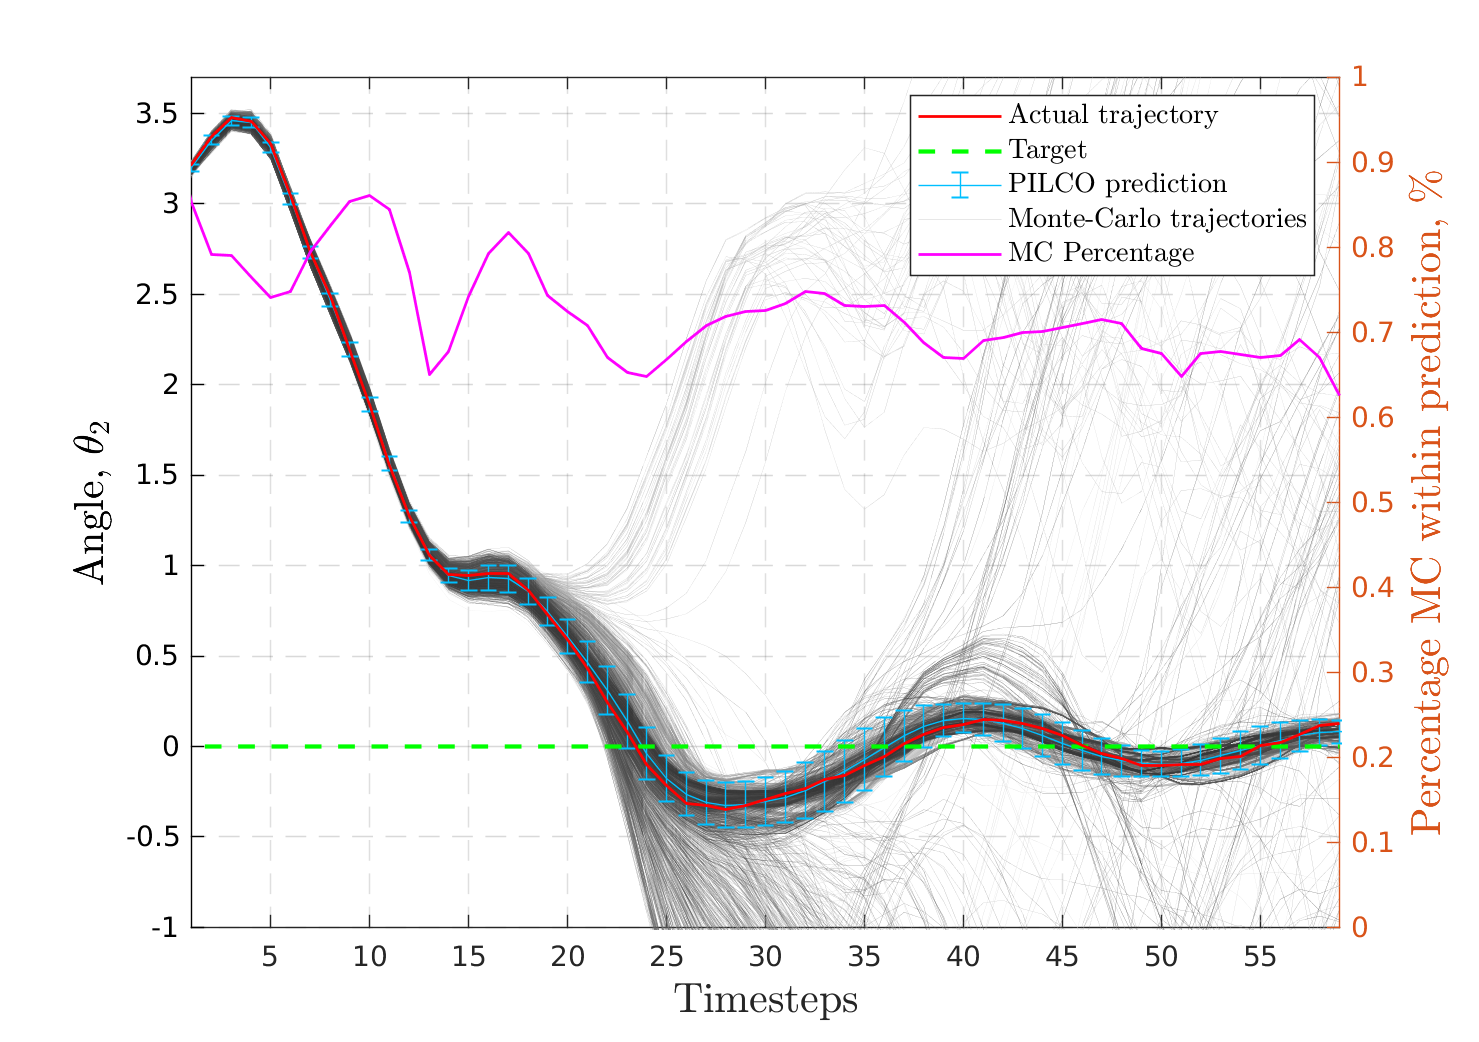
\includegraphics[height=0.22\textheight,width=1\textwidth]{Chapter3/Figures/pen_MC_rollout_Ep_40_Dim_3.png} 
    \caption{Pendulum angle $\theta_2$} 
    \label{Fig:Re-pen-pen-velocity} 
  \end{subfigure} 
  \hspace{\fill}
  \begin{subfigure}[b]{0.48\linewidth}
    \centering
    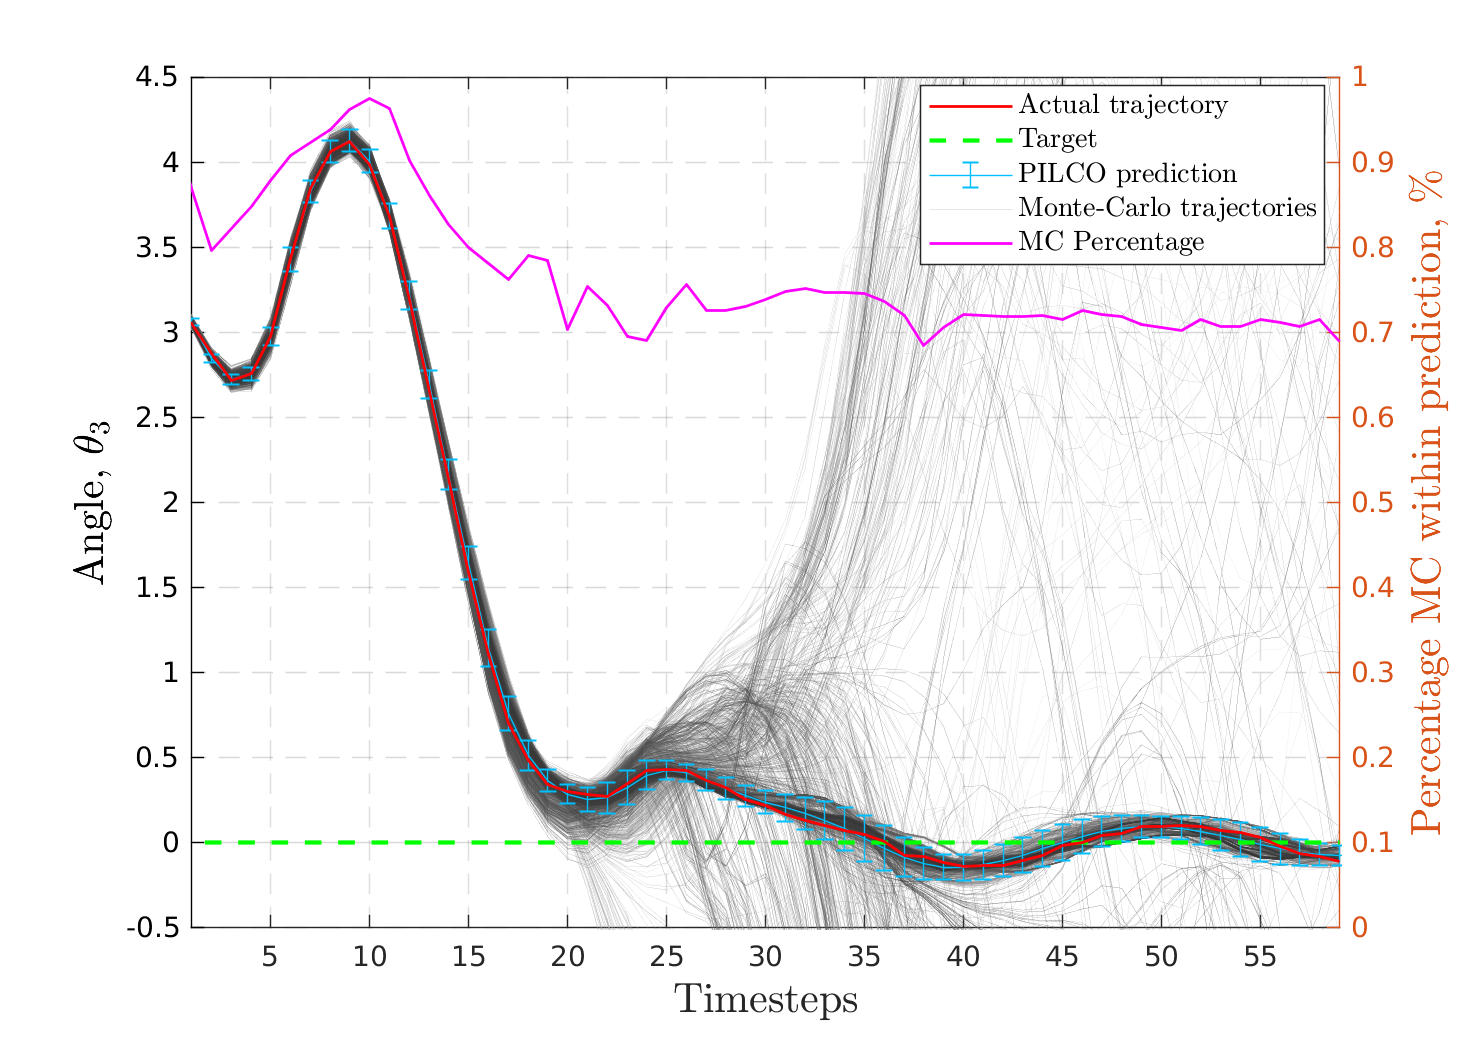
\includegraphics[height=0.22\textheight,width=1\textwidth]{Chapter3/Figures/pen_MC_rollout_Ep_40_Dim_4.png} 
    \caption{Pendulum angle $\theta_3$} 
    \label{Fig:Re-pen-pen-angle} 
  \end{subfigure} 

    \vspace{4ex}
  \begin{subfigure}[b]{0.48\linewidth}
    \centering
    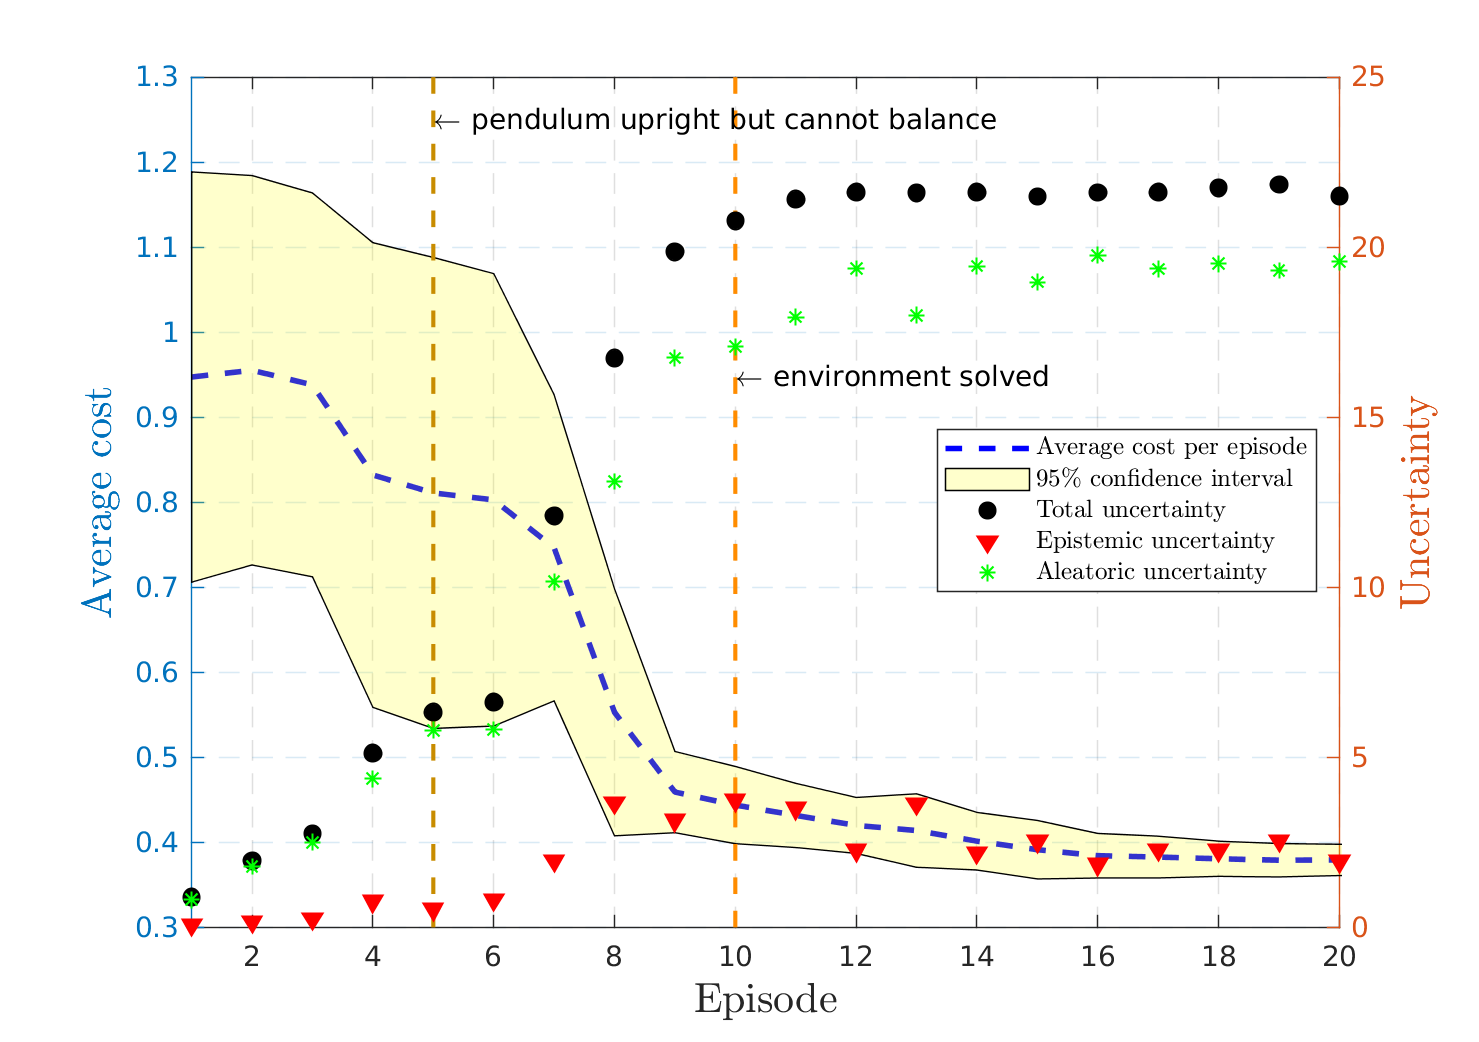
\includegraphics[height=0.22\textheight,width=1\textwidth]{Chapter3/Figures/pen_uncertainty.png} 
    \caption{Average cost (left axis) and uncertainty decomposition (right axis) for each episode over the course of learning.} 
    \label{Fig:Re-pen-uncertainty} 
  \end{subfigure}
  \hspace{\fill}
  \begin{subfigure}[b]{0.48\linewidth}
    \centering
    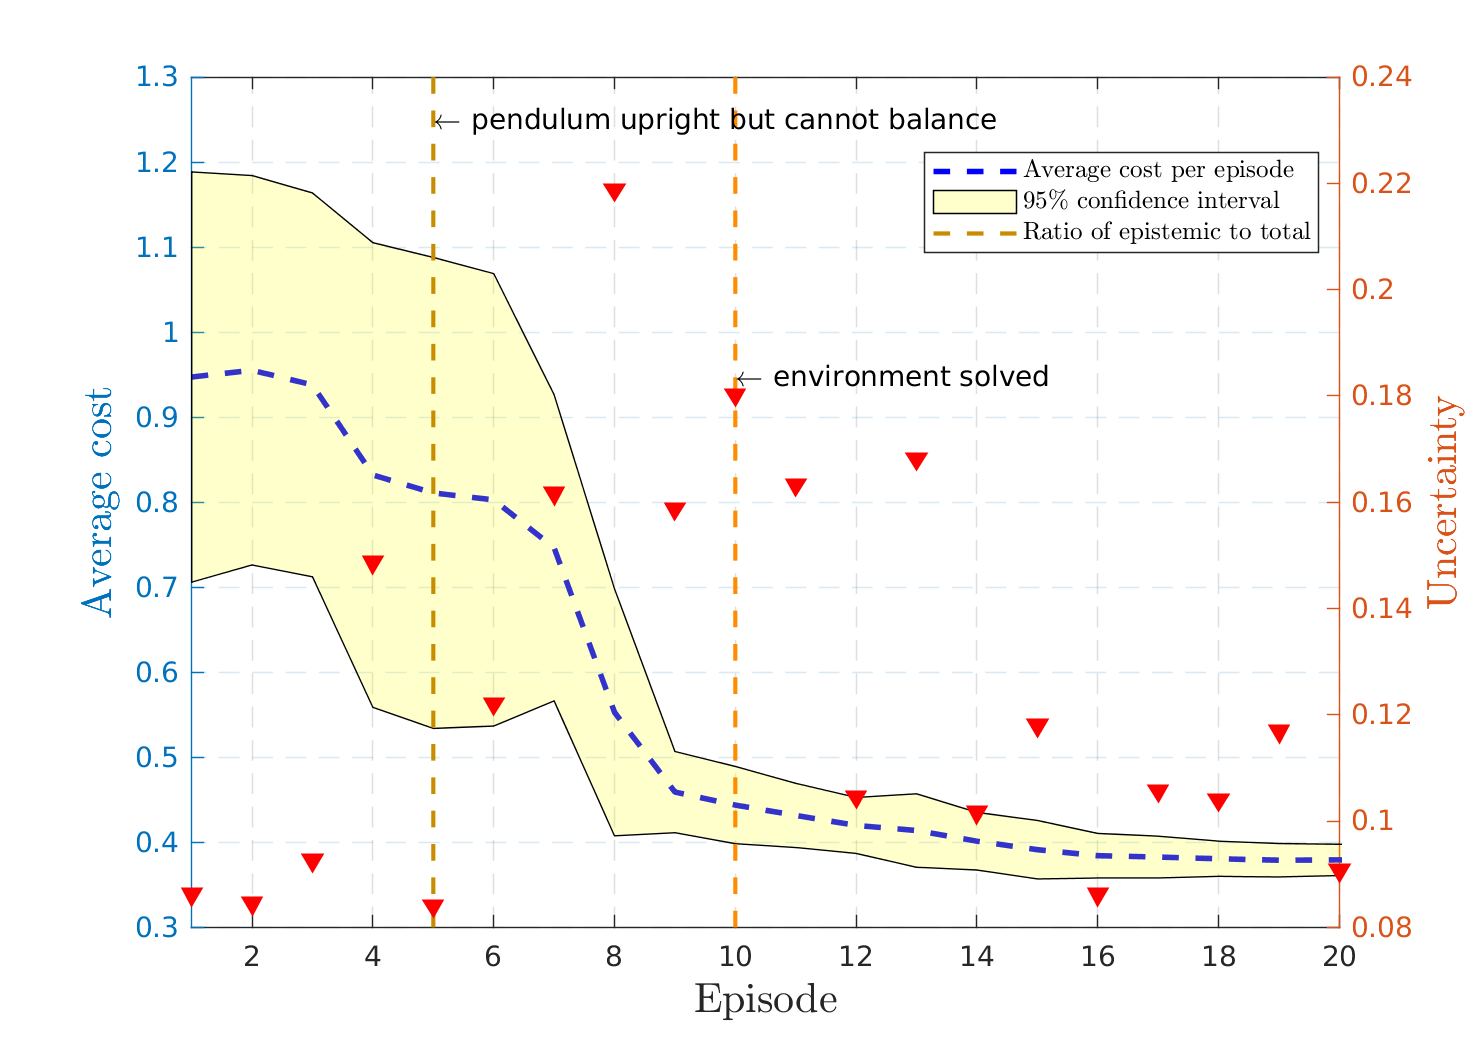
\includegraphics[height=0.22\textheight,width=1\textwidth]{Chapter3/Figures/pen_uncertainty_norm.png} 
    \caption{Average cost (left axis) and ratio of epistemic to total uncertainty (right axis) for each episode over the course of learning.} 
    \label{Fig:Re-pen-uncertainty-norm} 
  \end{subfigure} 
\caption[Monte-Carlo uncertainty decomposition for for \textbf{pendubot} environment]{Monte-Carlo uncertainty decomposition for the \textbf{pendubot} environment. Figs. \ref{Fig:Re-cp-cart-position} - \ref{Fig:Re-cp-pen-angle} show a random sample of the Monte-Carlo trajectories for each of the state variables for episode 20. The first three legend items (actual trajectory, target, PILCO prediction and MC trajectories) correspond to the state variable axis (left axis) and the magenta line shows the percentage of MC trajectories inside PILCO's prediction (2 standard deviations) (right axis). Figs. \ref{Fig:Re-cp-uncertainty} - \ref{Fig:Re-cp-uncertainty-norm} show the average cost (left axis) and uncertainty (right axis) for each episode over the course of learning.}
\label{Fig:Re-Pendubot-Full-Results} 
\end{figure}

\subsection{CartDoublePendulum}


\begin{figure}[htp!]    
  \begin{subfigure}[b]{0.48\linewidth}
    \centering
    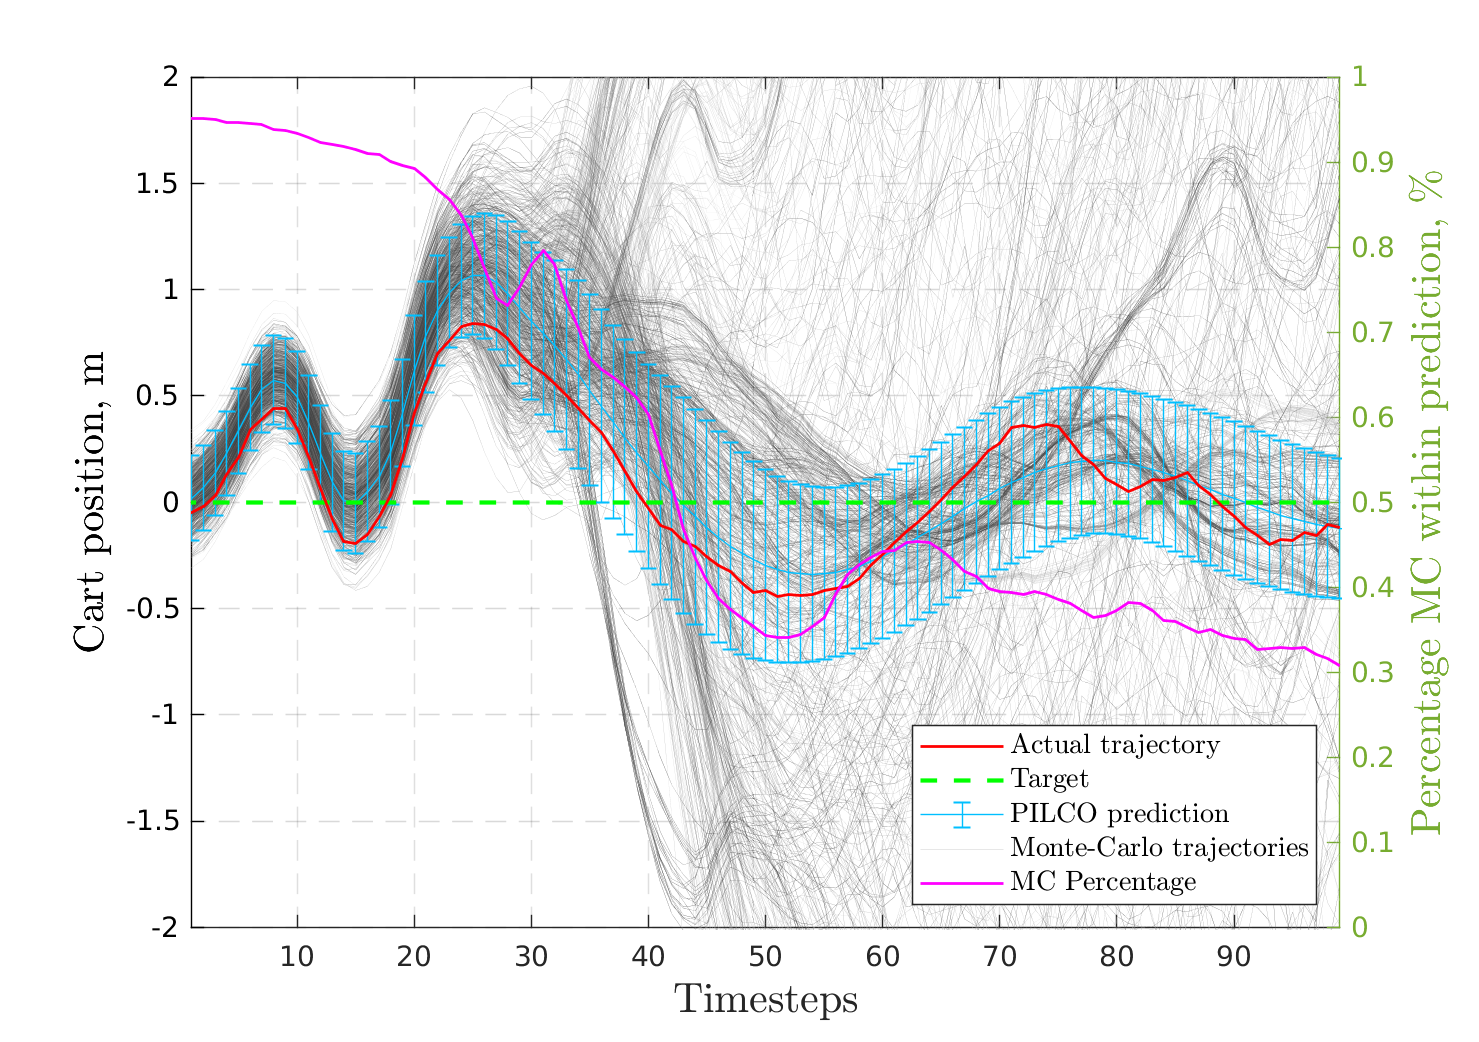
\includegraphics[height=0.22\textheight,width=1\textwidth]{Chapter3/Figures/cdp_MC_rollout_Ep_75_Dim_1.png} 
    \caption{Cart position $x_1$} 
    \label{Fig:Re-cdp-cart-position} 
  \end{subfigure} 
  \hspace{\fill}  %% maximize space between adjacent subfigures
  \begin{subfigure}[b]{0.48\linewidth}
    \centering
    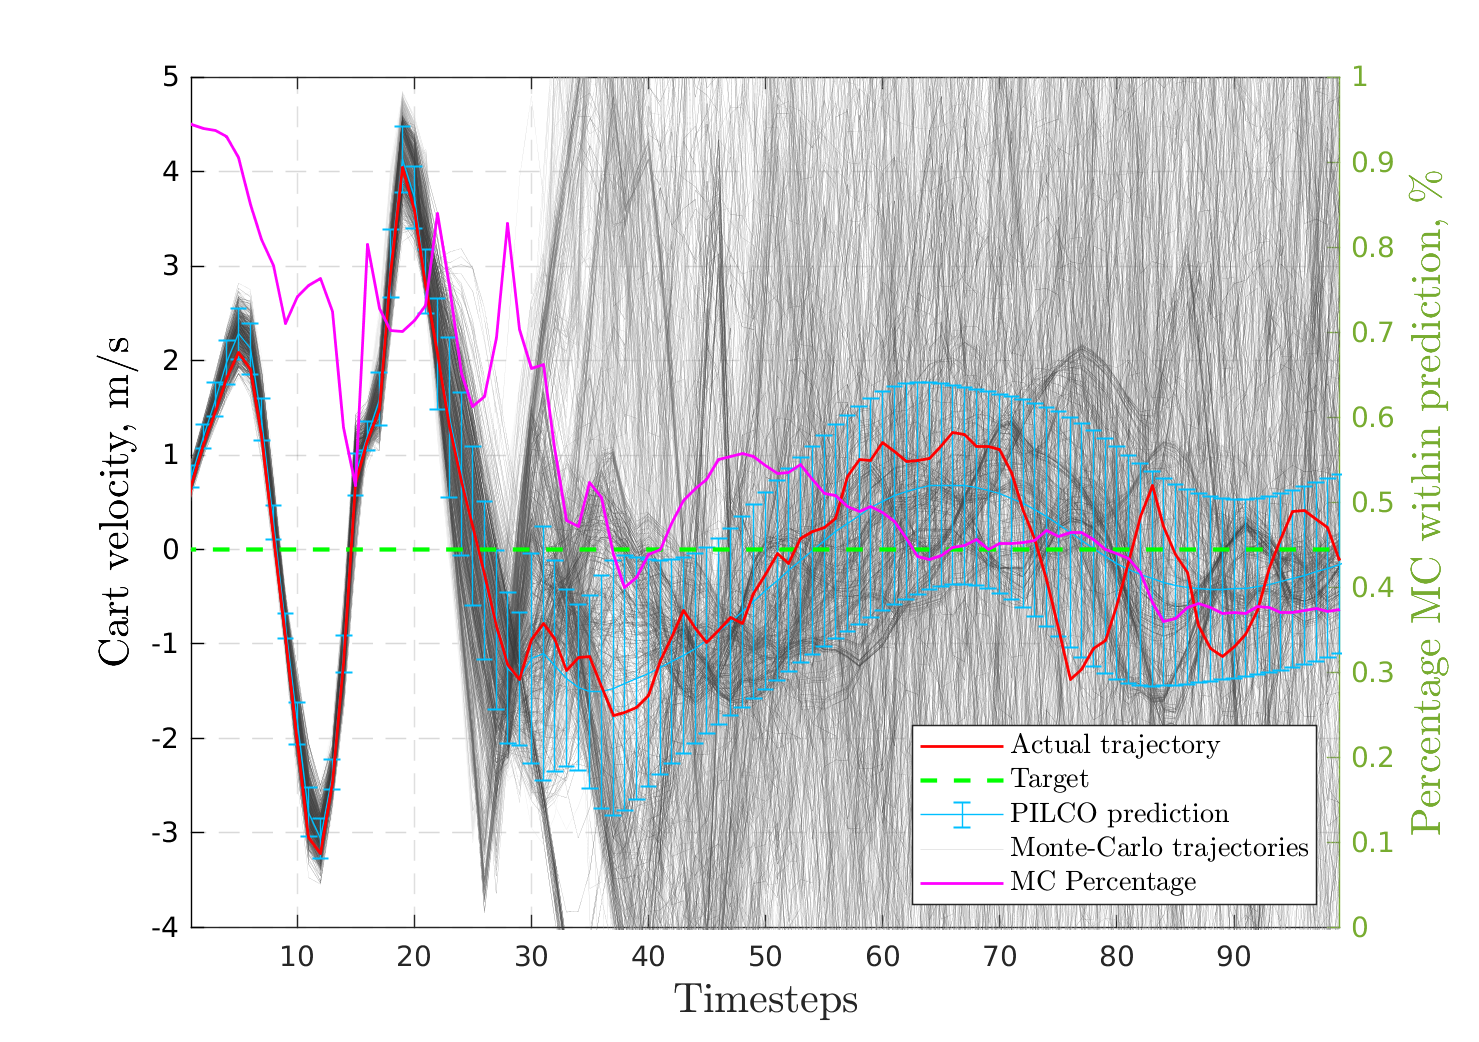
\includegraphics[height=0.22\textheight,width=1\textwidth]{Chapter3/Figures/cdp_MC_rollout_Ep_75_Dim_2.png} 
    \caption{Cart velocity $\dot{x}_1$} 
    \label{Fig:Re-cdp-cart-velocity} 
  \end{subfigure} 

  \vspace{4ex}  %% extra vertical space
  \begin{subfigure}[b]{0.48\linewidth}
    \centering
    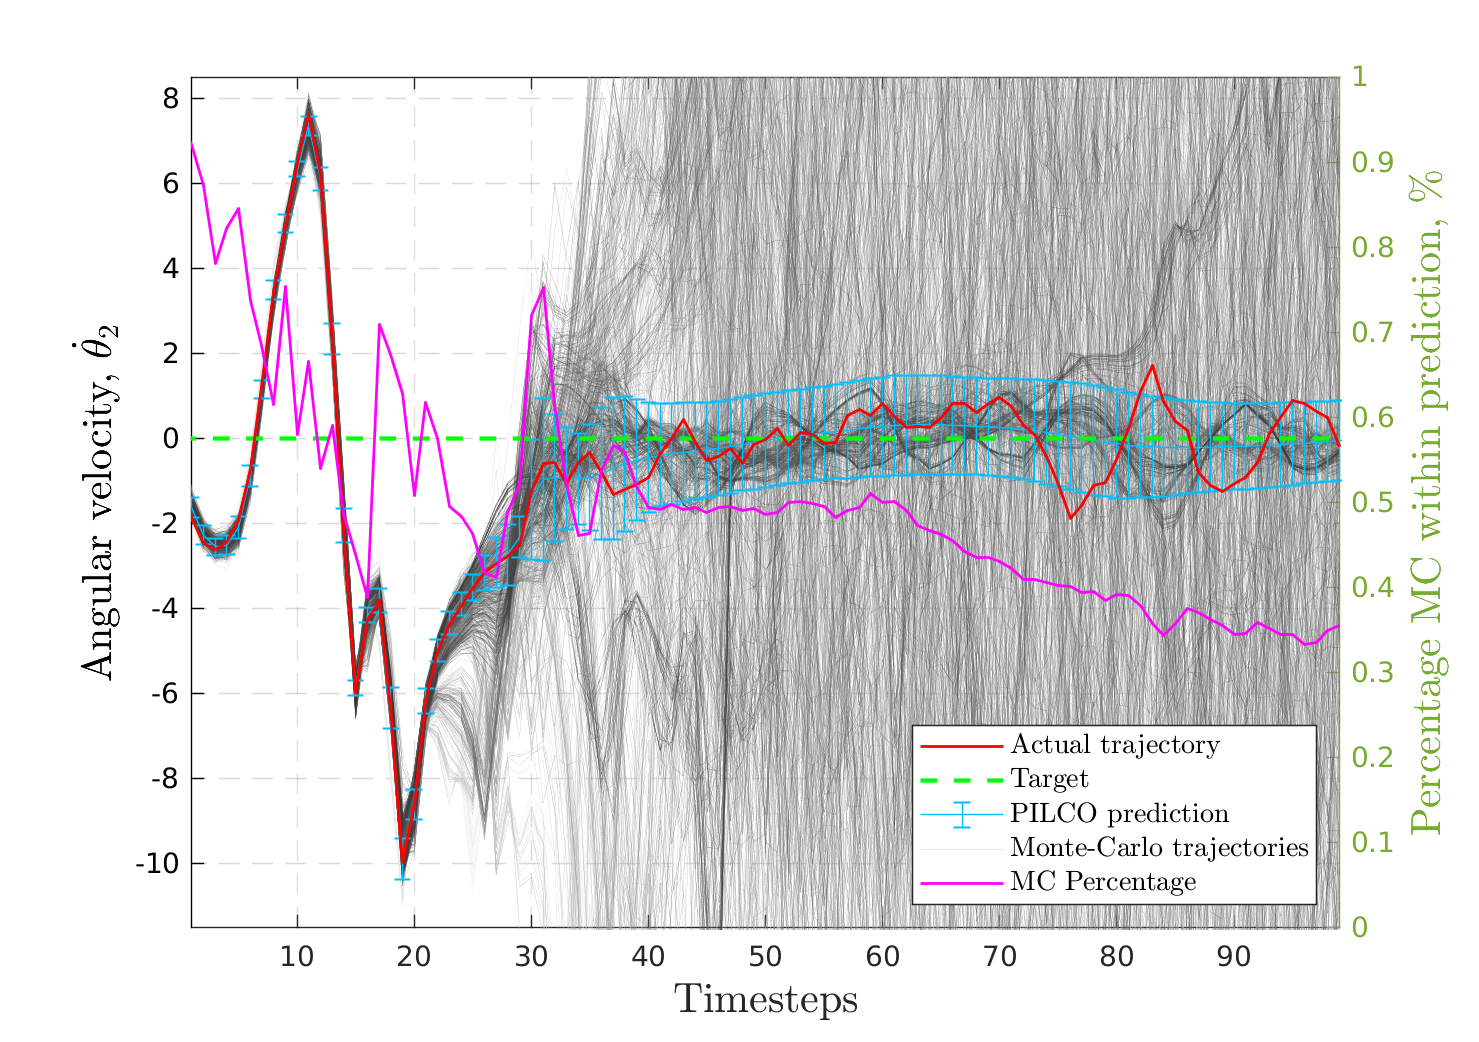
\includegraphics[height=0.22\textheight,width=1\textwidth]{Chapter3/Figures/cdp_MC_rollout_Ep_75_Dim_3.png} 
    \caption{Pendulum angular velocity $\dot{\theta}_2$} 
    \label{Fig:Re-cdp-pen2-velocity} 
  \end{subfigure} 
  \hspace{\fill}
  \begin{subfigure}[b]{0.48\linewidth}
    \centering
    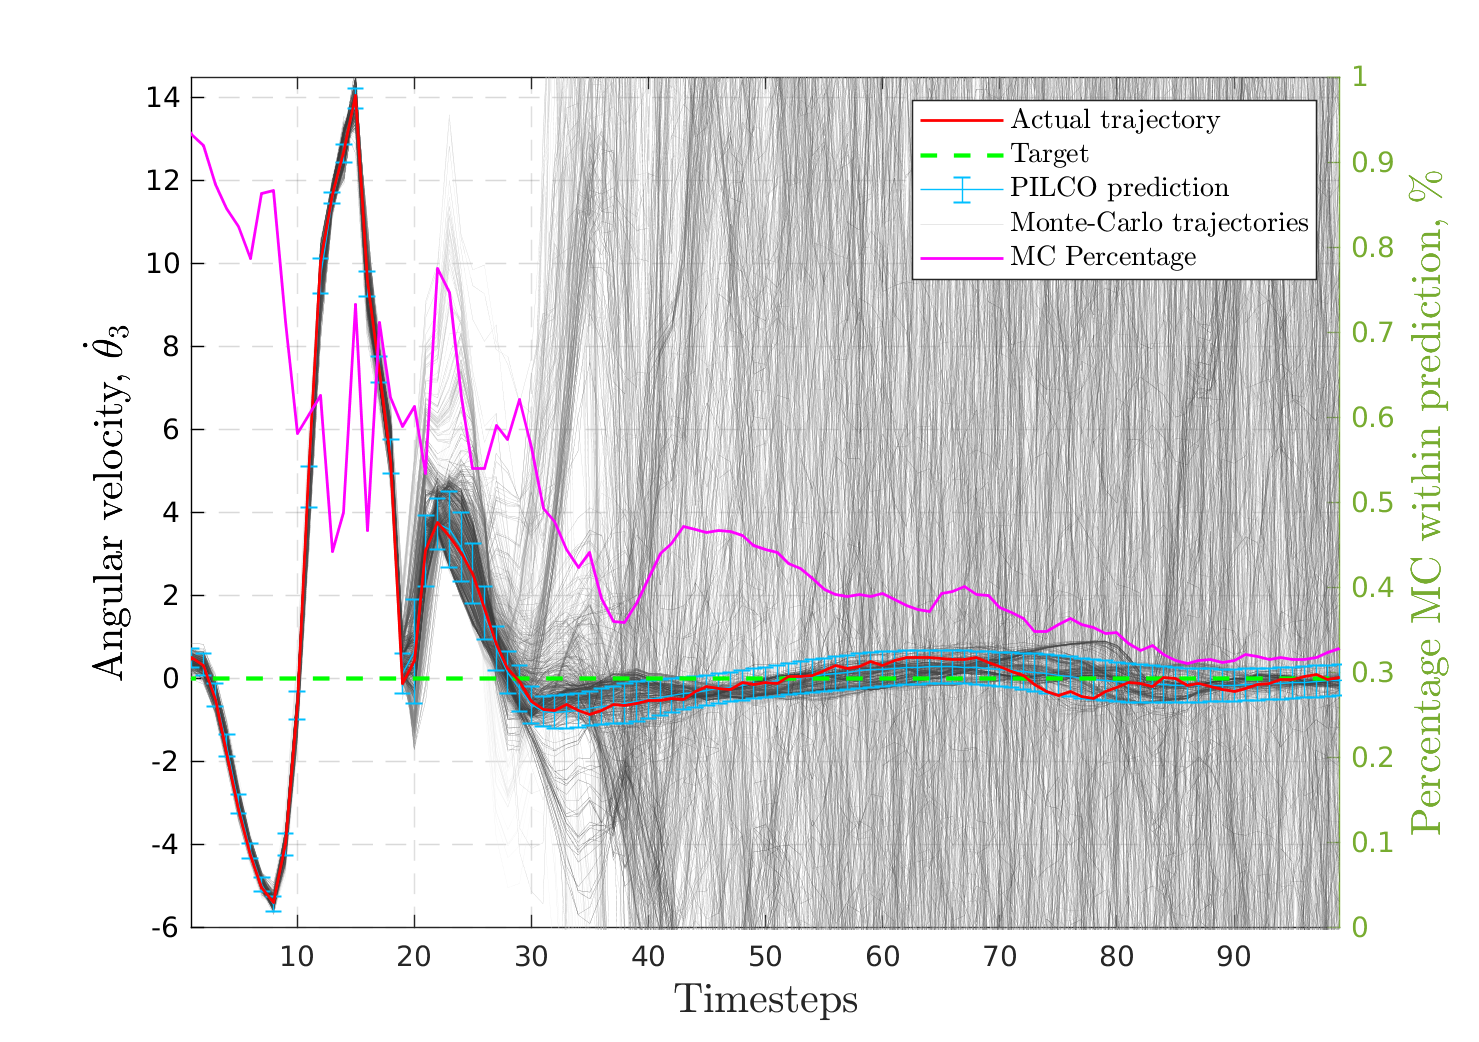
\includegraphics[height=0.22\textheight,width=1\textwidth]{Chapter3/Figures/cdp_MC_rollout_Ep_75_Dim_4.png} 
    \caption{Pendulum angular velocity $\dot{\theta}_3$} 
    \label{Fig:Re-cdp-pen3-velocity} 
  \end{subfigure} 

    \vspace{4ex}
  \begin{subfigure}[b]{0.48\linewidth}
    \centering
    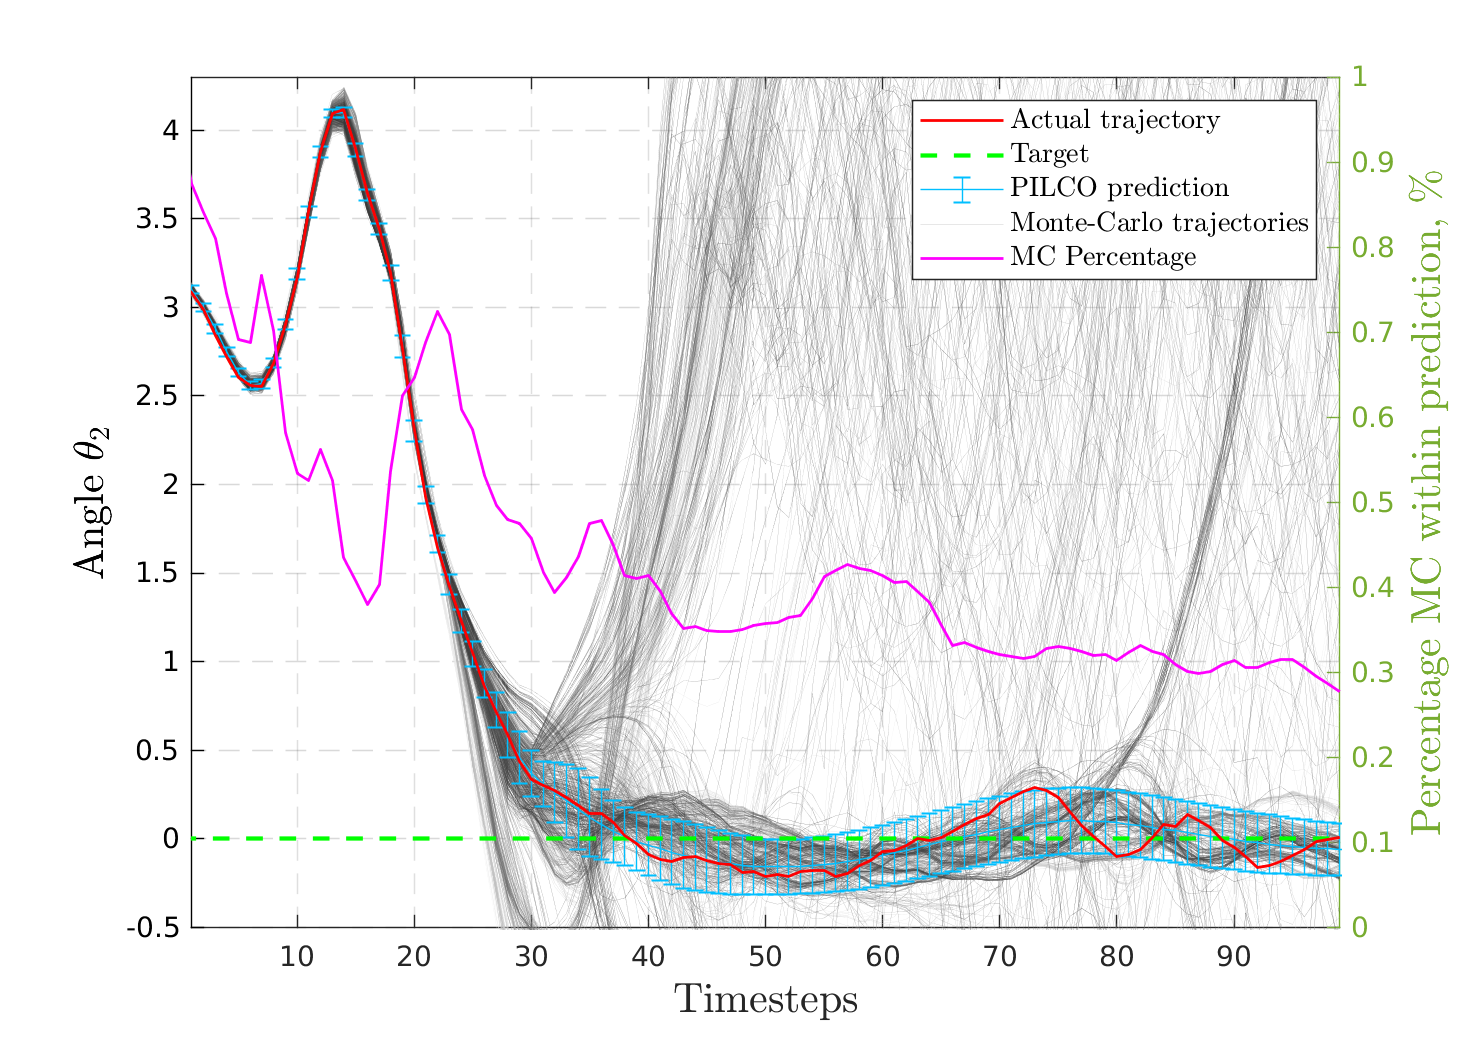
\includegraphics[height=0.22\textheight,width=1\textwidth]{Chapter3/Figures/cdp_MC_rollout_Ep_75_Dim_5.png} 
    \caption{Pendulum angle $\theta_2$} 
    \label{Fig:Re-cdp-angle2} 
  \end{subfigure}
  \hspace{\fill}
  \begin{subfigure}[b]{0.48\linewidth}
    \centering
    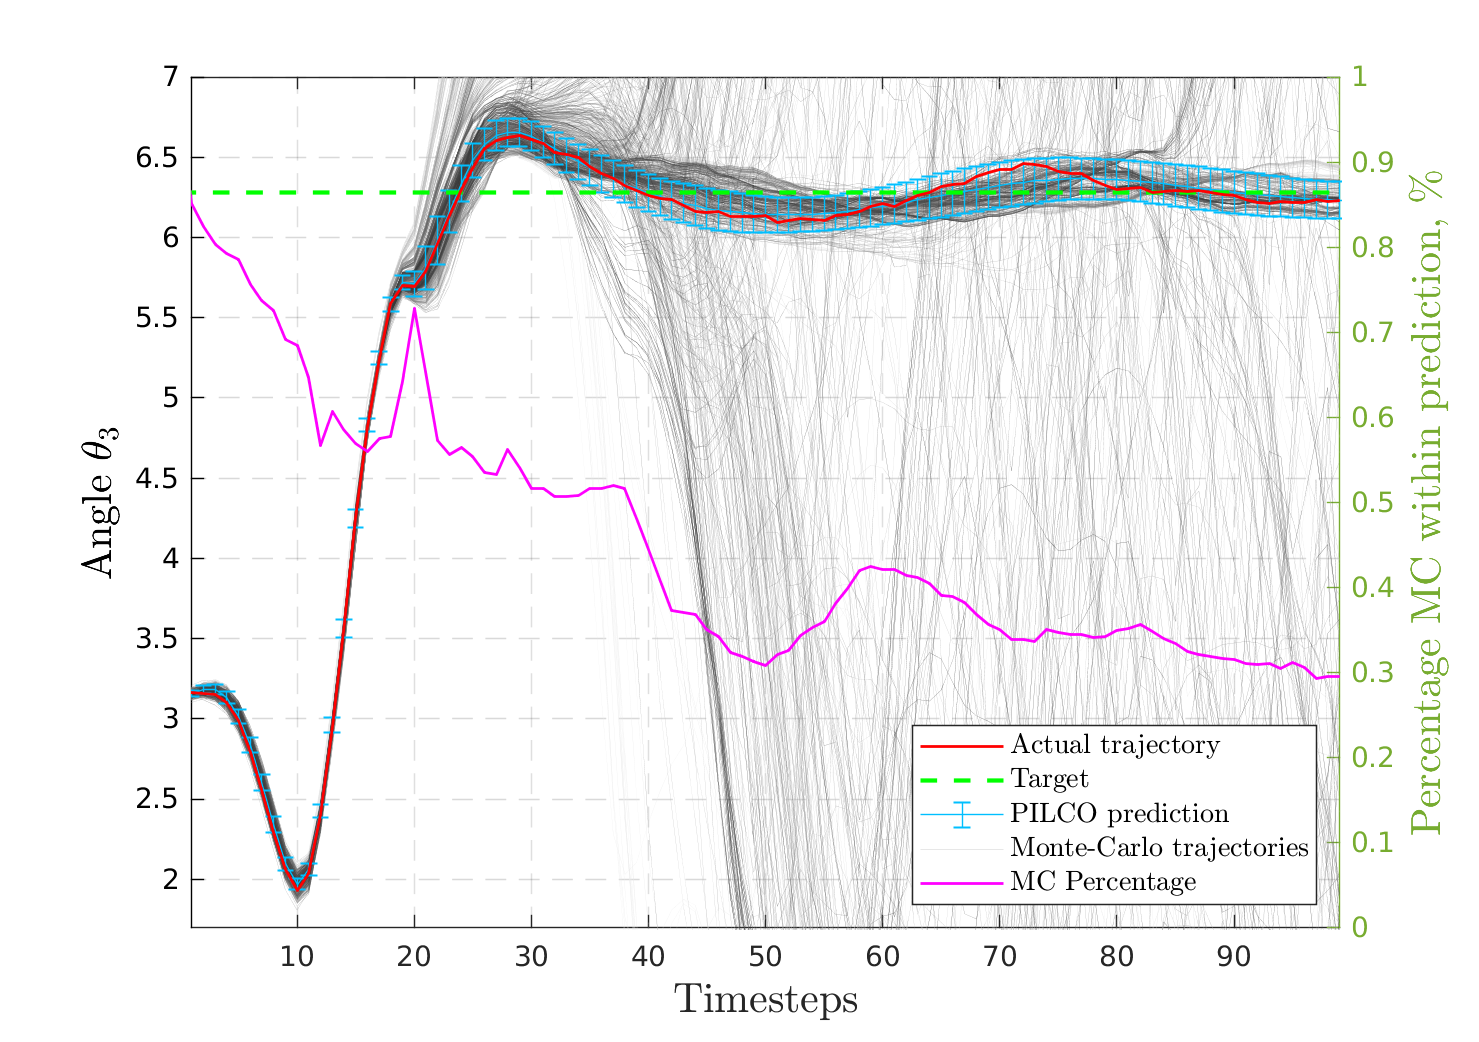
\includegraphics[height=0.22\textheight,width=1\textwidth]{Chapter3/Figures/cdp_MC_rollout_Ep_75_Dim_6.png} 
    \caption{Pendulum angle $\theta_3$} 
    \label{Fig:Re-cdp-angle3} 
  \end{subfigure} 
\caption[Monte-Carlo roll outs for \textbf{cart-double-pendulum} environment]{Monte-Carlo roll outs for the \textbf{cart-double-pendulum} environment. Figs. \ref{Fig:Re-cdp-cart-position} - \ref{Fig:Re-cdp-angle3} show a random sample of the Monte-Carlo trajectories for each of the state variables for episode 75. The first three legend items (actual trajectory, target, PILCO prediction and MC trajectories) correspond to the state variable axis (left axis) and the magenta line shows the percentage of MC trajectories inside PILCO's prediction (2 standard deviations) (right axis).}
\label{Fig:Re-CartDoublePen-MC-Rollouts} 
\end{figure}



\begin{figure}[htp!]    
  \begin{subfigure}[b]{1\linewidth}
    \centering
    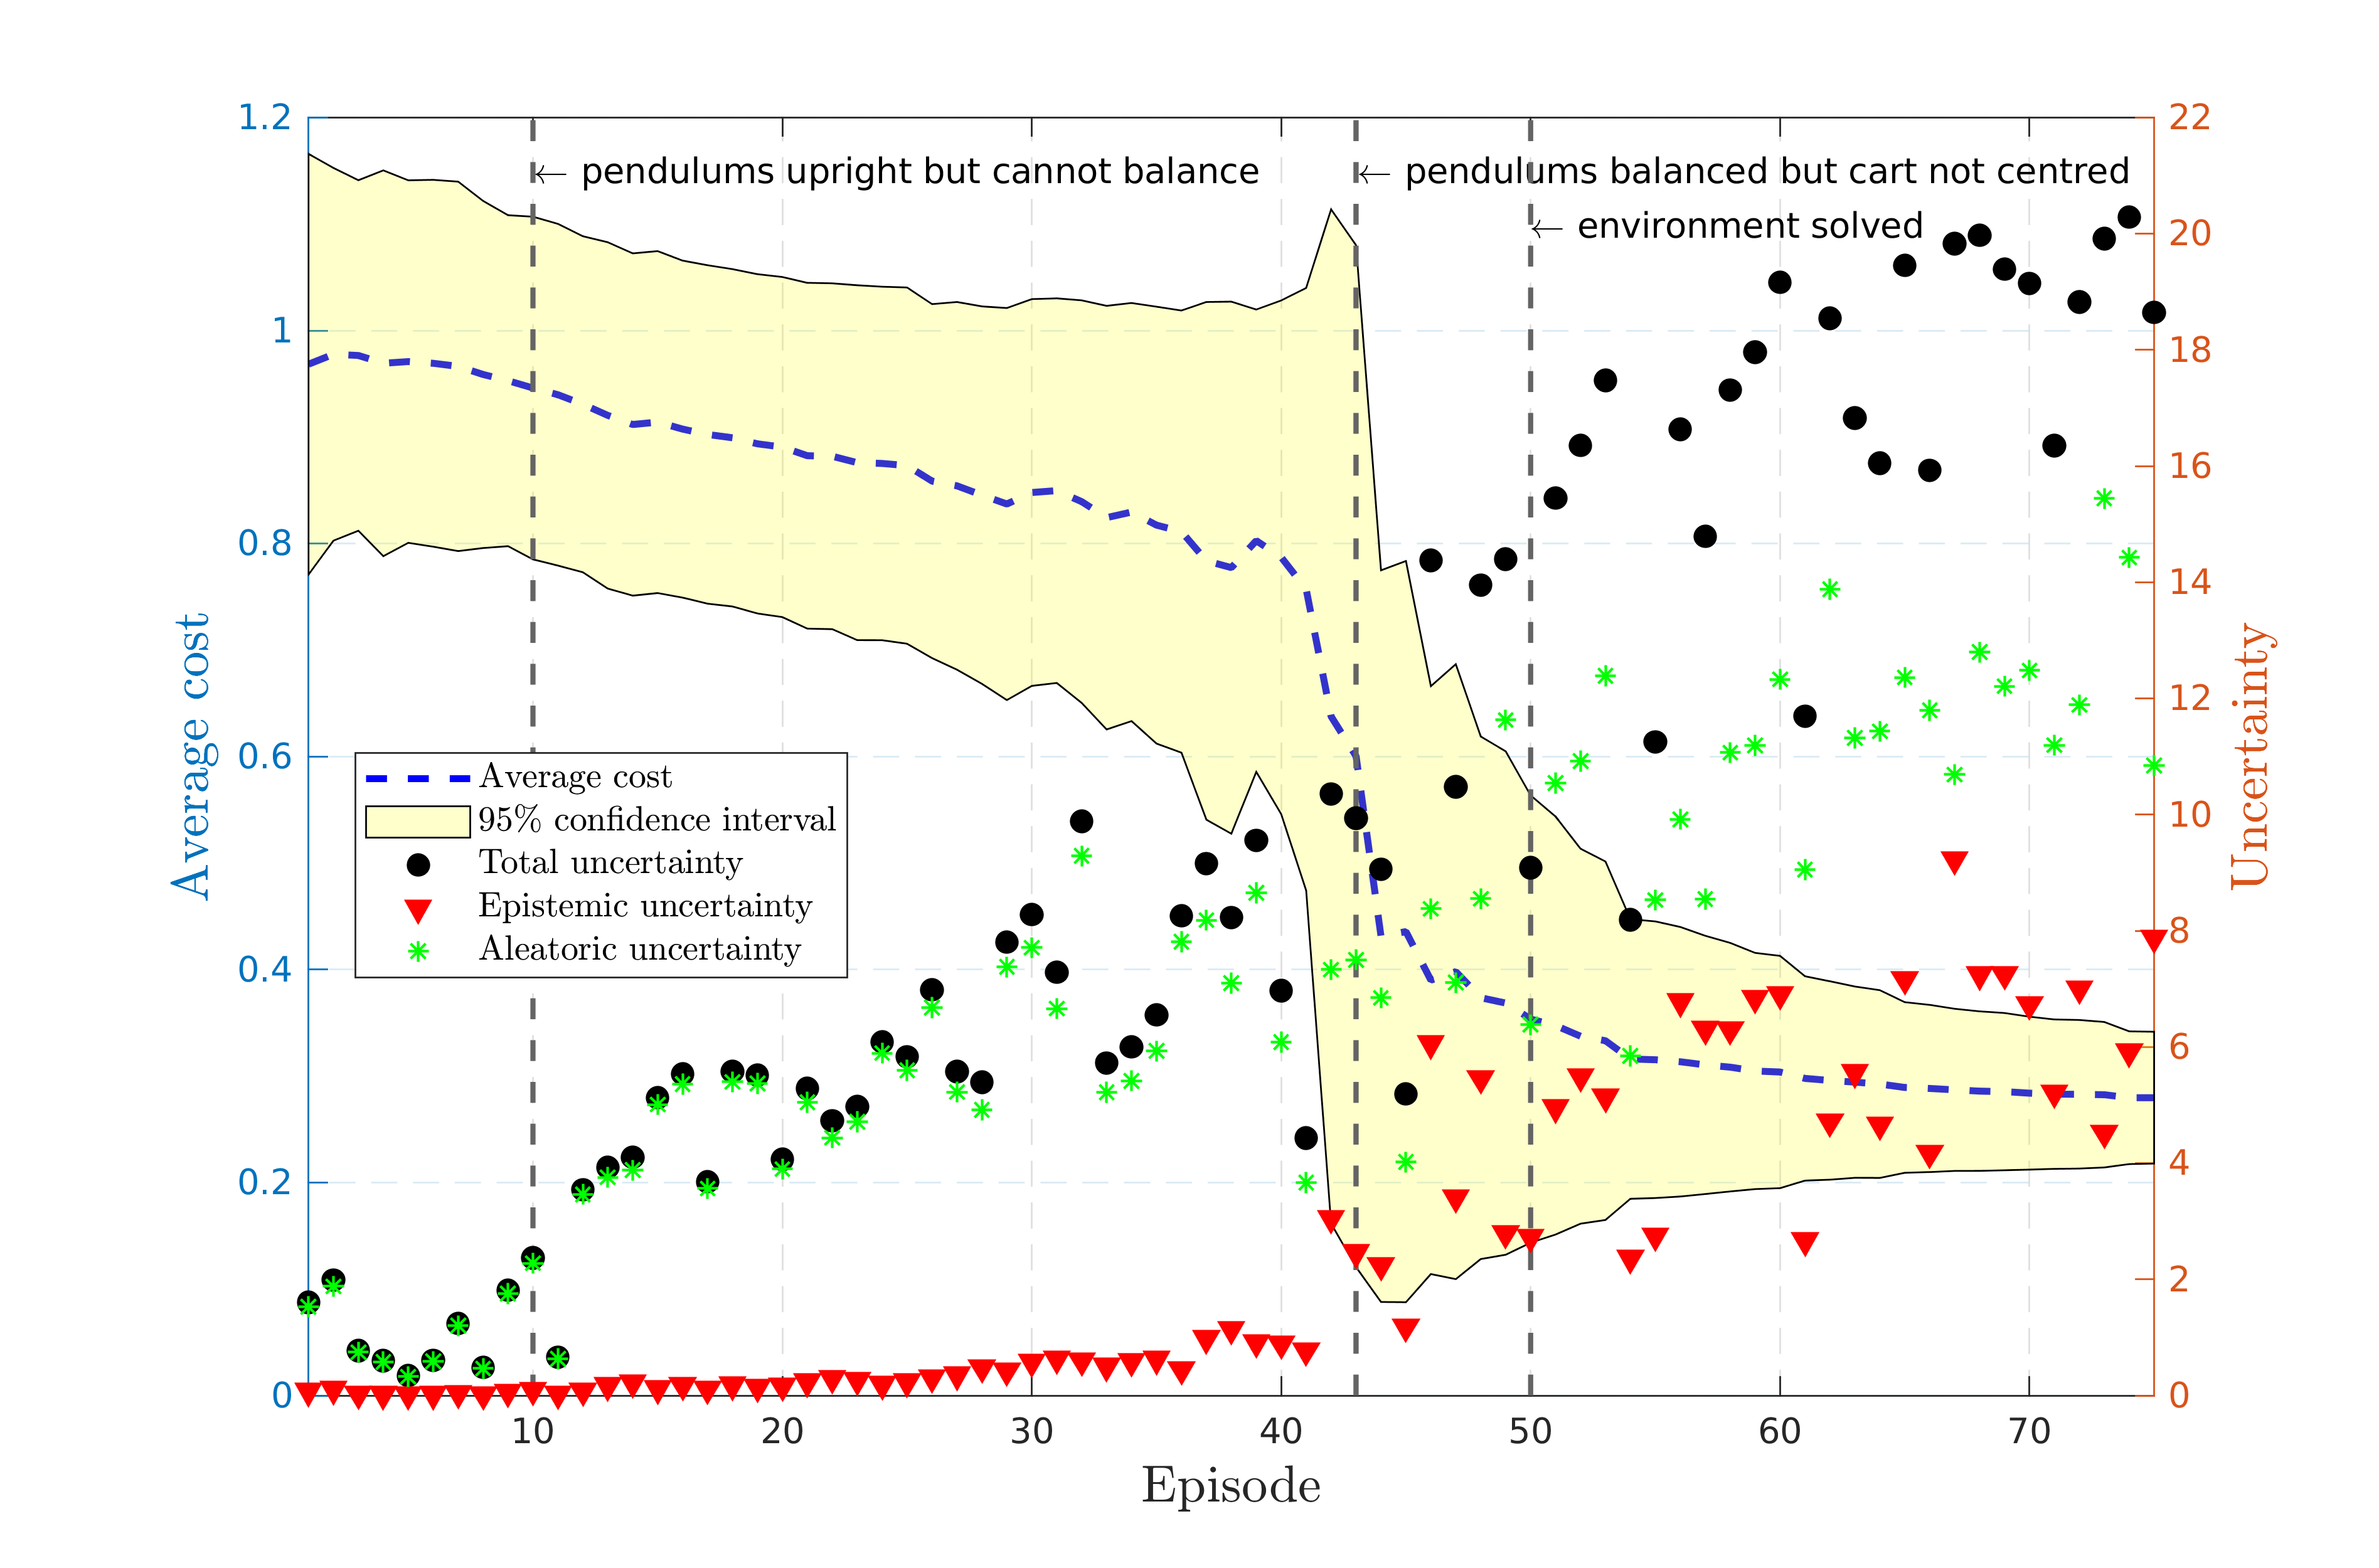
\includegraphics[height=0.4\textheight,width=1\textwidth]{Chapter3/Figures/cdp_uncertainty.png}
    \caption{Average cost (left axis) and uncertainty decomposition (right axis) for each episode over the course of learning.} 
    \label{Fig:Re-cdp-uncertainty-decomposition} 
  \end{subfigure} 

%   \vspace{4ex}  %% extra vertical space
  \begin{subfigure}[b]{1\linewidth}
    \centering
    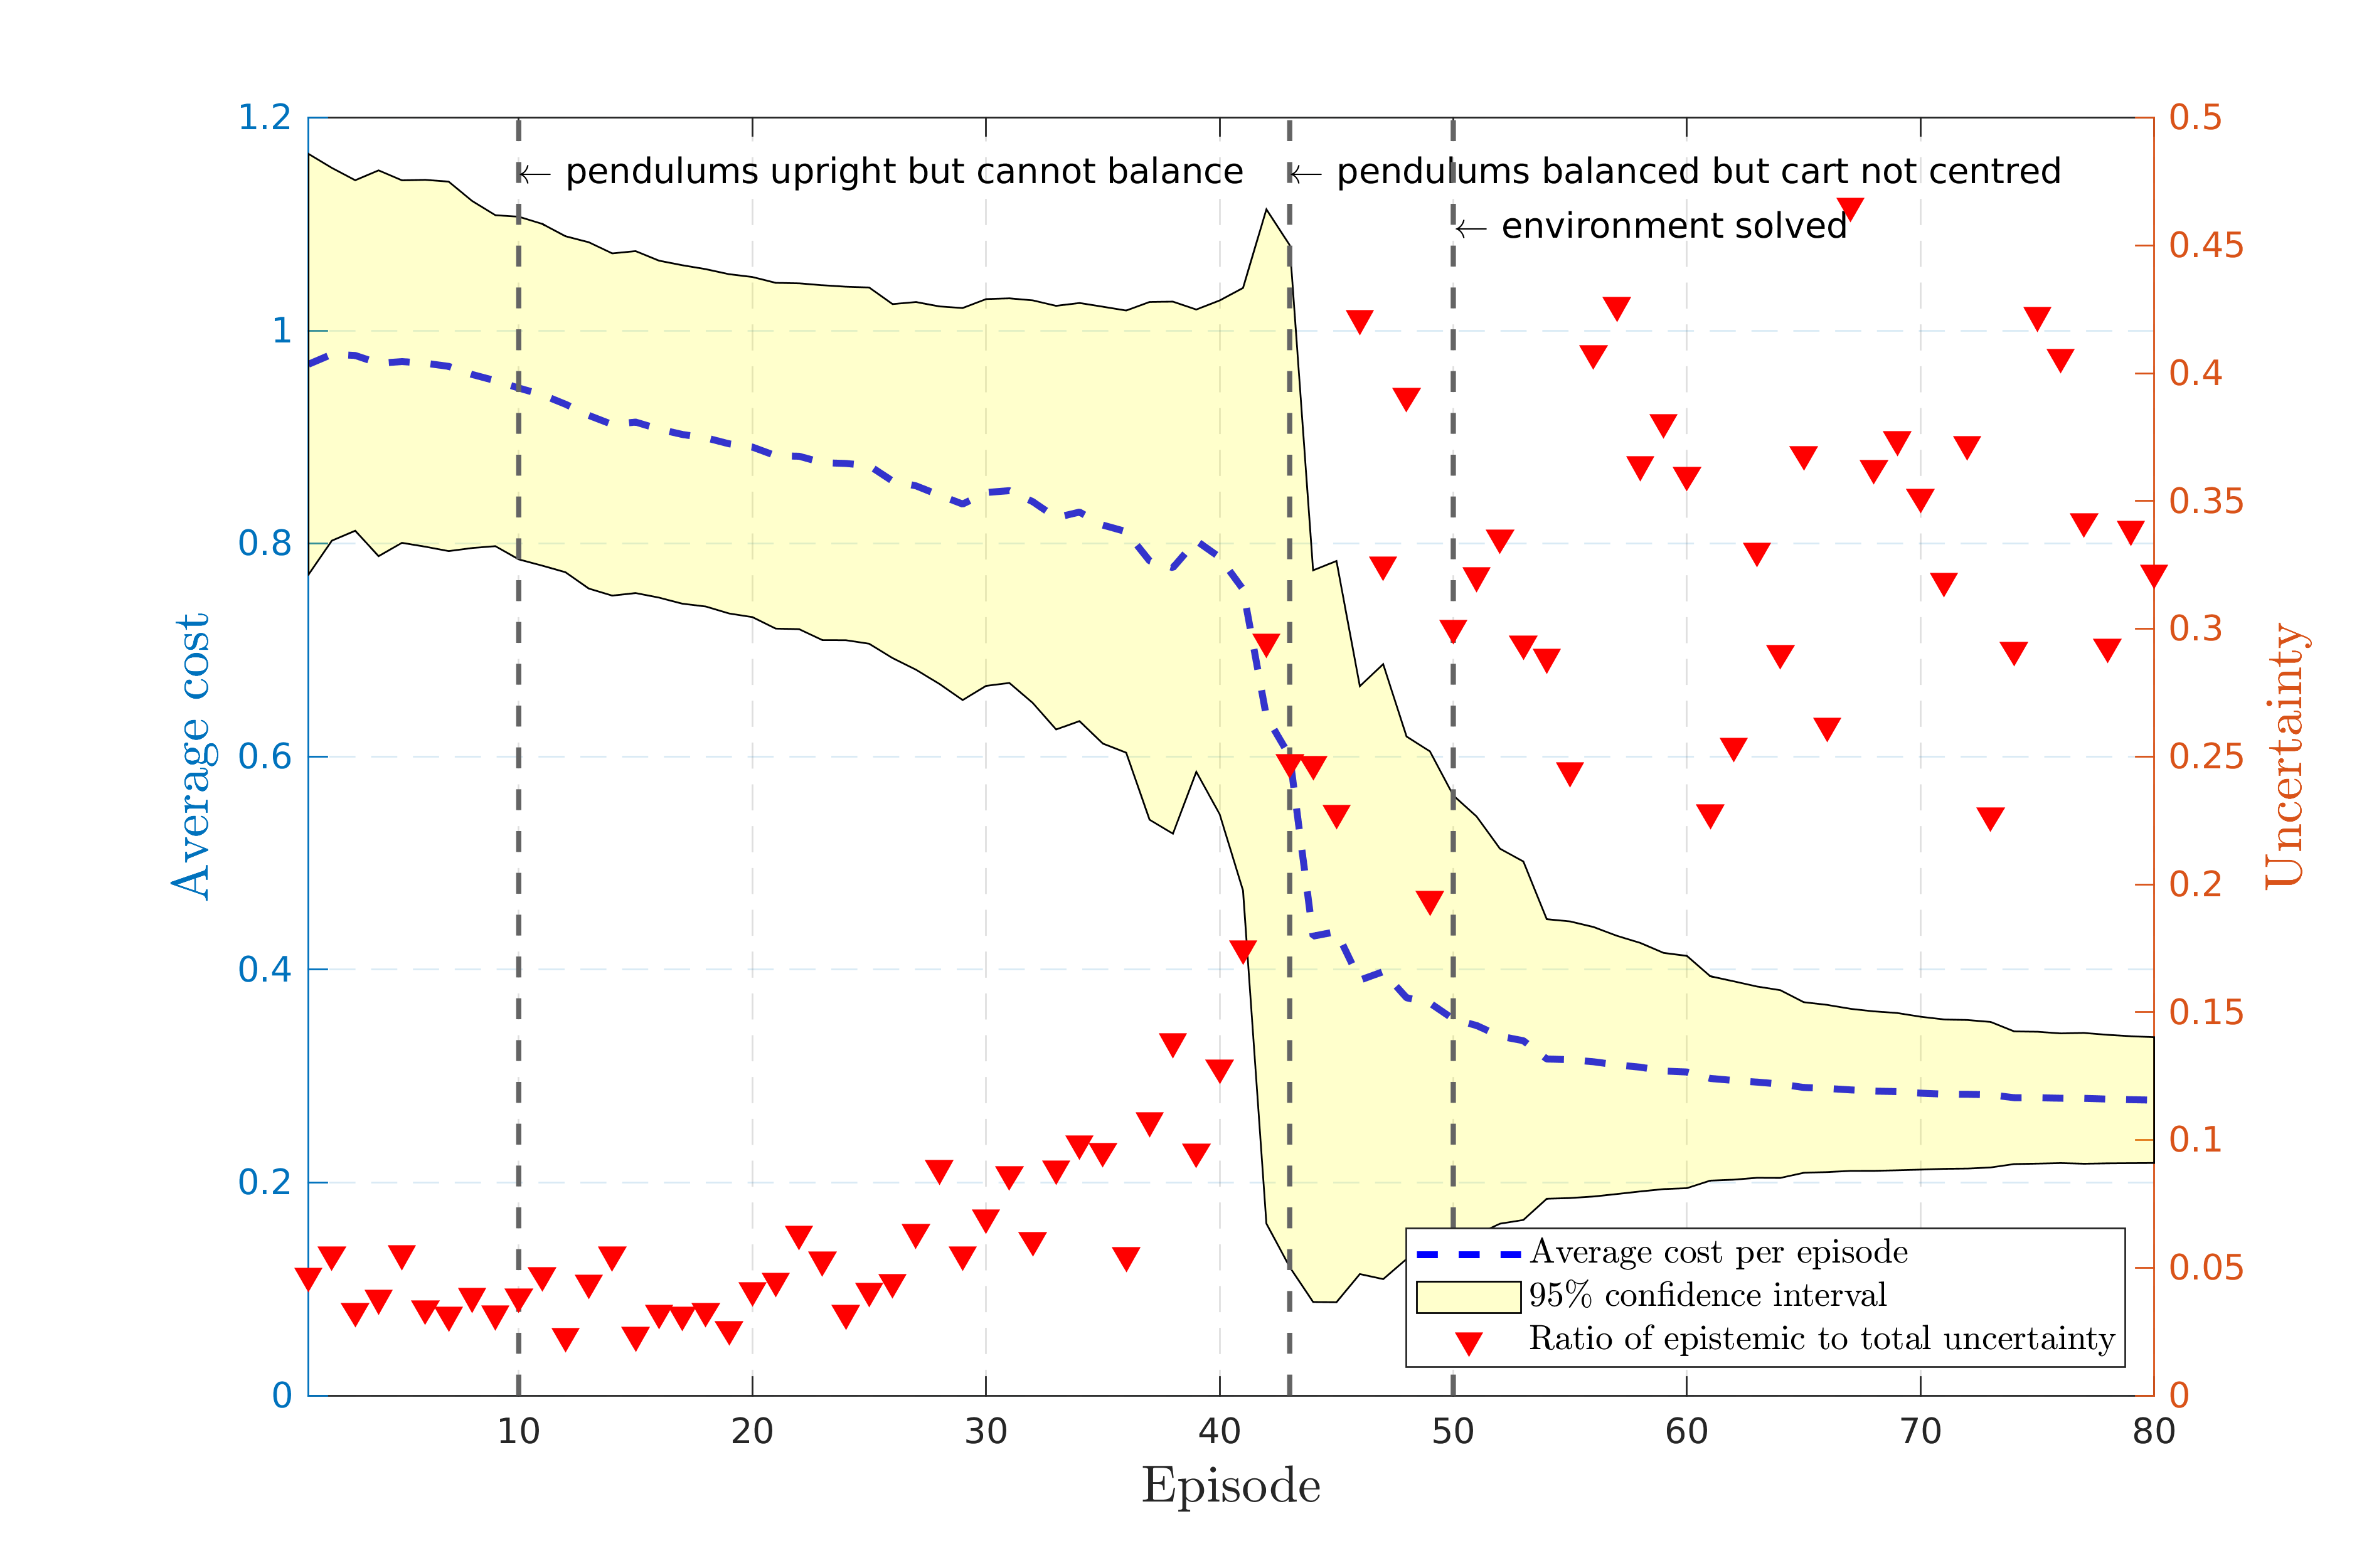
\includegraphics[height=0.4\textheight,width=1\textwidth]{Chapter3/Figures/cdp_uncertainty_normalised.png} 
    \caption{Average cost (left axis) and ratio of epistemic to total uncertainty (right axis) for each episode over the course of learning.} 
    \label{Fig:Re-cdp-uncertainty-normalised} 
  \end{subfigure} 
 
\caption[Monte-Carlo roll outs for \textbf{cart-double-pendulum} environment]{Monte-Carlo uncertainty decomposition for the \textbf{cart-double-pendulum} environment. Figs. \ref{Fig:Re-cdp-uncertainty-decomposition} - \ref{Fig:Re-cdp-uncertainty-normalised} show the average cost (left axis) and uncertainty (right axis) for each episode over the course of learning.}
\label{Fig:Re-CartDoublePen-Uncertainties} 
\end{figure}



RESULTS THAT I HAVE
\begin{itemize}
    \item Cartpole
\end{itemize}

A list of plots that I want:

\begin{itemize}
    \item Plots of number of basis functions for each environment used and maybe also convergence plots.
    \item Plot of a 1D transition function showing the distribution over trajectories on the side. Perhaps also a distribution over losses. I have the GP notebook to do this already.
    \item Plot showing 1D function with uncertainty breakdown and how it decreases with more data as we become more confident about the weights.
    \item For each environment, plot of the actual trajectories for the solved environment and a plot of the MC trajectories for the solved environment.
    \item Plots showing that when PILCO is not learning it is choosing policies with high reward but low epistemic uncertainty.
    \begin{itemize}
        \item How to achieve this: 
    \end{itemize}    
\end{itemize}

\section{Discussion}

\section{Conclusion}



